\bookpart{信号}{Signals}
\label{part:signals}

\BookPartGuide{%
本部分研究带位置和边界的数值对象。信号在位置、时间或索引上取值，读数必须连同位置
一起比较；一组数不能当作无序集合处理。

第~\ref{chap:signal-analysis}章“信号”先确定索引、通道与边界，再在时域、频域和多项式
三类表示之间转换；随后用范数、内积、能量与平均功率比较信号，讨论平移、缩放、线性时
不变卷积、相关以及网格、幅度和形态映射，并比较卷积的不同快速计算路线，最后研究采样
恢复的信息条件与抗混叠。

信号的分解和变换改变的是数值的表示，坐标可逆、卷积正确与连续信号可恢复是三类不同
要求。把函数放到图的顶点上以后，连接结构会进一步规定传播和比较发生在哪些位置；那是
下一“图”部分的内容。}

\chapter{信号}
\label{chap:signal-analysis}

一台传感器在不同时刻记下读数，就得到了一串有先后次序的数。
面对这样一串数，我们想问的问题往往并不一样：想知道异常发生在什么时候，
直接比较相邻读数即可；想知道振动究竟有多快，则要把整段记录拆成不同频率的波动。
前一种问法用的是各时刻的原始读数，后一种问法改用一组频率系数来描述同一条记录。
再往后，滤波会改变读数，采样则决定究竟能留下多少观测。
因此本章依次回答四个问题：怎样才算完整地描述一条信号，怎样比较两条信号，
怎样计算信号经过运算后的结果，以及只凭部分读数还能恢复出哪些信息。

为了让边界和位置的作用看得见、算得出，本章反复使用两条很短的有限记录
\begin{equation}
  \bm x=(1,2,1),\qquad \bm h=(1,-1)
  \label{eq:signal-analysis-running-example}
\end{equation}
作为贯穿例。确定了索引、取值和边界之后，脉冲、复指数和多项式会给出三套不同的坐标；
范数、内积以及能量、功率这些指标则分别回答不同口径下的比较问题。
对于已经确定的卷积映射，我们以直接求和为基准，比较五条计算路线，
重点看清乘法次数减少之后又额外付出了哪些变换与存储代价。
到采样部分，则要进一步区分“换一种坐标仍然可逆”和“观测本身可逆”这两件不同的事。
函数空间与线性坐标的一般背景可回查
第~\ref{chap:functional-analysis-and-approximation}章和第~\ref{chap:linear-algebra}章。
本章只处理带有规则时间或位置索引的对象；下一章再把位置之间的关系推广为一般的图，
并比较规则平移与图上传播的差别。若要用内部状态描述一个响应，需要先给定初始状态、
状态更新和输出读取规则，输入输出映射才能完全确定，相关工具可参考
\BookChapterRef{chap:dynamical-systems-and-state-estimation}{卷2《数学准备：概率、因果与决策》的“动力系统”章}。

规则位置不一定只有一条时间轴：图像有两个空间方向，视频还兼有时间方向。
这时频率相应地成为向量，而局部窗口、反射边界和分辨率改变又会挑选不同的坐标。
我们先把一维的四类变换讲清楚，再推广到网格；余弦坐标、短时频谱和多尺度分解
则分别用来处理边界、定位与细节。运算部分还会讨论网格差分、有限精度取值
以及局部集合上的非线性变换；采样部分最后逐一检验这些表示或运算能否消除观测上的歧义。

\section{信号的对象与表示}
\label{sec:signal-objects-structure}

在此前的章节里，向量、矩阵和函数大多被当作现成的数学对象使用，
我们很少追问一个数组里的“第几个数”究竟意味着什么。本章的数据却总是带着位置：
一段音频每秒记录若干次读数，一张灰度图在每行每列记录亮度，一段文本把每个词映射成向量。
它们的共同点是，单凭数值本身无法确定它记录了哪个对象，还必须知道数值在什么位置取得、
同一时刻有几个通道一起读数、整段记录之外又该补上什么。把位置也纳入对象的定义之后，
许多运算才有确定的含义。

先用一个具体场景说明为什么非这样不可。设想一台温度记录仪每秒写下一个读数，
十分钟后得到六百个数。若只把这六百个数看成一个无序集合，我们就答不出
“温度上升最快的是哪一段”，因为“哪一段”依赖先后次序；也答不出
“这条记录和昨天那条有多像”，因为比较至少要把对应位置对齐。
一旦把位置显式记录下来，读数就不再是孤立的数字，而成为以位置为自变量的对象，
这就是本章要研究的\term{信号}（signal）。索引确定之后，我们才能区分连续取值与等间隔取值、
单通道与多通道、有限记录与无限序列，并据此挑选合适的表示和算法。

位置带来次序，也带来本章反复处理的两类问题。其一，比较两条记录时，
看峰值、看绝对值之和还是看平方和，会选出不同的“更大者”；
其二，平滑、求导、卷积这类运算只把每个位置附近的读数按权重汇总，
朴素地在长记录上逐个计算代价很高，需要换成频率或多项式坐标来复用中间结果。
下面先确定对象，再约定比较口径，然后研究运算及其快速计算，最后考察采样究竟丢失了什么。

\subsection{信号的索引与取值}

同一个数组既可能记录不同时刻的温度，也可能记录同一时刻多个传感器的读数；
数组首尾是否相接，同样会改变它所代表的对象。因此在讨论用位置值、频率系数
或多项式坐标表示信号之前，要先把索引、取值和边界三件事说清楚。

\subsubsection{连续、离散与有限信号}

传感器可以在每个时刻都读出一个值，也可以只在约定的时刻保留读数。
把时间或位置当作自变量、把读数当作函数值，就得到前面所说的信号。
连续时间记作$x(t)$，整数位置记作$x[k]$。需要留意，“连续时间”说的是允许读取的时刻，
而不是波形不能有突跳；一个开关在某一时刻突然从零变为一，仍然是连续时间信号。

\begin{definition}[信号的索引类型]
  \label{def:signal-index-types}
  连续时间标量信号是$x:I\to\mathbb F$，其中$I\subseteq\mathbb R$为时间区间，
  $\mathbb F$取$\mathbb R$或$\mathbb C$。
  \term{离散时间信号}（discrete-time signal）是$x:\mathbb Z\to\mathbb F$，
  或定义在明确指定的整数子集上。对正整数$N$，长度$N$的有限信号是
  $x:\{0,\ldots,N-1\}\to\mathbb F$，可按位置写成$\bm x\in\mathbb F^N$。
\end{definition}

整数下标本身并不携带物理时间。若第$k$项来自时刻$t_0+kT_s$，
那么起点$t_0$和正的采样间隔$T_s>0$共同确定了真实的采样时刻，
也决定了“每隔两项重复一次”对应多快的物理振荡。不等间隔观测则必须显式保存每个时间戳，
不能直接套用均匀采样的公式。二维图像用两个整数坐标标记位置，规则网格上的运算
可以相应推广到$\mathbb Z^d$；但一般图节点的编号并不自带这种平移结构。

位置次序本身就是信号的一部分。$(1,2,1)$和$(1,1,2)$含有相同的数值和出现次数，
可相邻位置的差分别是$(1,-1)$与$(0,1)$。只保存取值的集合或计数，就会丢掉这一差别；
局部差分和模板比较都要求把位置保留下来。

随机信号则是在概率空间上给每个索引配一个随机变量；固定一次随机结果$\omega_0$后，
$k\mapsto X_k(\omega_0)$成为一条确定路径。对这条路径求频谱，与对随机信号求期望，
是两种不同的操作，一次观察不会自动给出总体规律。本章先研究给定的确定信号；
随机变量与期望可参考\BookChapterRef{chap:random-variables}{卷2《数学准备：概率、因果与决策》的“随机变量与概率基础”章}，
过程和路径的表示可参考\BookChapterRef{chap:random-sequences-and-processes}{卷2《数学准备：概率、因果与决策》的“随机序列与随机过程”章}。

复数值常用来同时记录两个实分量，或者表示一次振荡的幅度与相位。
用复数描述振荡并不是追求形式上的一般化：一个实余弦只能告诉你“此刻多大”，
却无法在一次乘法里同时表达“多大”和“正处在振荡的哪个阶段”；
写成复指数之后，平移、缩放等操作都只对应乘以一个复数，幅度和相位被同一个数一并携带，
后面频域中“平移只改变相位”的结论正依赖这一点。
记$\mathrm i^2=-1$，对$z=a+\mathrm ib$有
$\overline z=a-\mathrm ib$、$|z|^2=z\overline z=a^2+b^2$。
这里的\term{复共轭}（complex conjugate）只改变虚部的符号，并不是时间反转；
后文内积中之所以要取共轭，正是为了让自内积得到非负的大小。

本章沿用第~\ref{sec:linear-algebra-length-angle-distance}节及
第~\ref{chap:functional-analysis-and-approximation}章的复内积约定：
第一变量共轭线性，第二变量线性。沿正交归一方向$u$读取信号$x$的系数写作
$\langle u,x\rangle$。后文把模板$h$与信号片段作内积时，也把模板放在第一变量的位置，
使读数对信号片段保持线性；这样既与全卷约定一致，也保留了相关运算中对模板取共轭的公式。

\subsubsection{单通道与多通道信号}

立体声在同一时刻有左、右两路读数。若把两路首尾接成一条长序列，
就会把通道之间的差别误当成时间上的先后，因此时间和通道这两种索引必须分别记录。
\begin{definition}[标量信号与向量值信号]
  \label{def:signal-multichannel}
  单通道信号在每个位置取一个标量值。设通道数$d$为正整数，$d$通道信号在每个位置取向量值
  $\bm x[k]=(x_1[k],\ldots,x_d[k])^\top\in\mathbb F^d$；
  连续时间时相应写作$\bm x(t)$。
  $N$个位置的记录可写为$\bm X\in\mathbb F^{N\times d}$，
  约定$\bm X_{k+1,c}=x_c[k]$，其中$k=0,\ldots,N-1$、$c=1,\ldots,d$。
\end{definition}

时间轴长度$N$与通道数$d$承担不同角色，二者不能互换。比如
\begin{equation}
  \bm X=
  \begin{bmatrix}1&0\\2&1\\1&2\end{bmatrix}
  \label{eq:signal-multichannel-record}
\end{equation}
有三个时刻、两个通道；第二行$(2,1)$是同一时刻两个通道的联合读数。
把多个传感器放进同一个向量，隐含着它们已经按同一时间基准对齐；
若第二通道延迟了一个采样间隔，就应先保留这一偏移，不能把不同时刻的值当成同时观测。
多通道既不意味着各通道彼此独立，也不意味着必须逐通道处理：
既可以对每一列分别滤波，也可以在每个时刻用一个矩阵把多个通道混合起来。
后者的输入输出维度以及它在时间上的作用，将在第~\ref{sec:signal-input-output-maps}节明确区分。

\subsection{信号的周期与边界}

\subsubsection{周期信号与非周期信号}

一段记录里出现两次相似的峰形，只能说明这两个局部片段彼此接近。
周期性要求严格得多：存在同一个平移量，使整个信号在平移后精确重复。
要写出这一要求，定义域也必须允许按该量反复平移。
\begin{definition}[周期及基本周期]
  \label{def:signal-period}
  定义在$\mathbb R$上的信号$x$若存在$T>0$使$x(t+T)=x(t)$对所有$t$成立，
  则称其为周期信号，$T$为一个周期。
  定义在$\mathbb Z$上的信号若存在正整数$N$使$x[k+N]=x[k]$对所有整数$k$成立，
  则称其为周期序列。若所有正周期中存在最小者，才称其为基本周期。
  没有正周期的信号称为非周期信号。
\end{definition}

在按几乎处处相等来识别函数的空间里，周期等式也按几乎处处理解。
常数连续信号的每个正实数都是周期，因而不存在最小正周期；
离散周期的候选是正整数，只要周期集合非空就一定有最小者。
连续复指数$e^{\mathrm i\Omega t}$在$\Omega\neq0$时的基本周期是
$2\pi/|\Omega|$；离散复指数$e^{\mathrm i\omega k}$则要求
$e^{\mathrm i\omega N}=1$，即$\omega/(2\pi)$为有理数，才有整数周期。
所以连续振荡取样之后是否仍然周期，取决于取样间隔与振荡周期之比。

多通道信号的周期要求所有通道共享一个共同周期。例如
\[
  \bm x(t)=\begin{pmatrix}\cos t\\\cos(\sqrt2\,t)\end{pmatrix}
\]
的每个分量单独看都是周期的，但共同周期必须同时满足$T=2\pi m$和
$\sqrt2 T=2\pi n$，其中$m,n$为整数；无理数$\sqrt2$使这样的正$T$不可能存在。
离散的有限多个周期通道则可取各整数周期的最小公倍数作为共同周期。

周期条件可以来自对象本身，也可以来自一种表示约定。一个真实过程可能持续重复；
一段有限数组也可以人为地首尾相接，当作一个周期来使用。这两种重复都发生在时间轴上。
后面的傅里叶表示里还会出现频率轴上的周期重复，那是时间索引取整数所导致的。
因此判断“在哪里发生了回绕”时，要说清楚周期条件约束的是原信号、有限坐标还是频率表示。

\subsubsection{有限支撑与边界延拓}

有限记录只说明了观测范围。要计算跨过首尾的运算，还必须交代区间之外取什么值。
关键在于：只拿到一段数组时，“第一个输入之前是什么、最后一个输入之后是什么”
并没有天然答案，而卷积、频谱等运算恰恰会用到区间之外的假想输入；
所以边界延拓不是可有可无的实现细节，它本身就是被处理信号定义的一部分。
离散信号的支撑是$\{k:x[k]\neq0\}$；只有有限个非零位置时称为有限支撑。
连续信号通常以非零集合的闭包定义支撑，在$L^p$类中则使用忽略零测差别的本质支撑。
因而连续时间的有限支撑是指支撑包含于某个有界区间，而不是只有有限个非零点。

对$x[0],\ldots,x[N-1]$，零延拓规定区间外的值为零；
周期延拓规定$x[k]=x[k\bmod N]$；反射延拓则把边界附近的值镜像放到区间外。
反射本身又有不同的端点约定。先沿数组走到右端、再折返到左端，可以写出一个完整周期。
不重复端点且$N\geq2$时，把
$(x[0],\ldots,x[N-1],x[N-2],\ldots,x[1])$
按周期$2(N-1)$延续，$N=2$时其中的折返段为空。
重复端点时，则把$(x[0],\ldots,x[N-1],x[N-1],\ldots,x[0])$
按周期$2N$延续。任意整数索引都先对相应周期取模，再读取该周期中的值。
例如记录$(1,2,1)$在$k=-2$处，两种反射分别给出$1$和$2$；
在$k=-1$处则分别给出$2$和$1$。若$N=1$，约定反射延拓恒等于唯一读数。
两种镜像都可能合理，但对应的不是同一个输入。

回到贯穿例$(1,2,1)$：零延拓后位置$0$左边相邻的值为$0$，周期延拓时为$1$，
不重复端点的反射延拓时为$2$。在位置$0$计算“当前值减前值”，三者分别得到
$1,0,-1$。这个差别在运算之前就已经确定，不能靠之后选用哪种快速算法来决定。

输出裁剪是另一项独立选择：先按给定延拓算出输出，再只保留指定位置。
裁掉首尾并不等于改变了输入延拓；保持输出长度相同，也不能唯一决定左右两侧怎样补值。
周期索引上的运算只在一个周期内计数；若把两条周期延拓序列直接放在整轴上无穷求和，
同一份贡献会被重复计无穷次。这一边界在循环卷积的定义中会继续保留。

\subsection{信号的时域表示}
\label{sec:signal-time-impulses}

有限记录可以逐位置拆开：只保留某个位置的读数、把其他位置暂时置零，
再把这些只含一个位置的记录相加，就恢复了原数组。
为什么要做这种看似平凡的拆分？因为它把“在某一时刻打入一个单位输入，
会怎样影响此后所有时刻”这个问题，化成了若干可以分别计算、再叠加起来的基本块；
后面卷积和线性时不变系统的整套理论，都建立在
“先求单个位置单位输入的响应，再按位置加权叠加”这一思路上。
为了让每个位置都能使用同一套表示，我们把仅在原点为一的信号移动到相应位置。
对整数$r$，约定平移算子为
\[
  (T_rx)[k]=x[k-r].
\]
$r>0$时，原来位于$k$的值移动到$k+r$，所以它表示延迟。
单位脉冲定义为
\[
  \delta[k]=
  \begin{cases}
    1,&k=0,\\
    0,&k\neq0.
  \end{cases}
\]
于是$T_r\delta[k]=\delta[k-r]$只在位置$r$非零。任意有限支撑信号都有展开
\begin{equation}
  x[k]=\sum_{r\in\mathbb Z}x[r]\delta[k-r].
  \label{eq:signal-analysis-impulse-expansion}
\end{equation}
例如贯穿输入就是$\delta[k]+2\delta[k-1]+\delta[k-2]$。
对每个固定的$k$，只有$r=k$那一项留下；对有限支撑输入，整个表达式还是有限和。
后面遇到允许叠加的系统时，就可以分别计算这些脉冲的输出再相加。

先固定长度$N$的记录：限制在这$N$个位置上的脉冲构成$N$维坐标空间的一组标准正交基，
展开系数就是原来的读数，因此完整展开可逆。若只保留位置集合$S$，被丢弃的位置就会带来误差。
记截断结果为$x_S[k]=x[k]\mathbb I_S(k)$，按第~\ref{chap:linear-algebra}章的欧氏范数计算，有
\[
  \|x-x_S\|_2^2=\sum_{k\notin S}|x[k]|^2.
\]
这才是投影近似的确切含义：未保留的位置进入误差。对$x=(1,2,1)$只保留中间位置，
近似为$(0,2,0)$，平方误差为$2$。保留一个时域系数与保留一个频域系数，舍弃的是不同方向，
不能只凭系数个数比较误差大小。
记$\ell_2(\mathbb Z)$为满足$\sum_r|x[r]|^2<\infty$的序列空间。对$x\in\ell_2$，
对称截断$\sum_{|r|\leq K}x[r]T_r\delta$在$\ell_2$中趋于$x$；
这是尾部平方和趋于零的结果，并不是对任意信号都成立的无条件范数收敛。

\subsection{信号的频域表示}
\label{sec:signal-analysis-frequency-representation}

脉冲展开把信号写成一组互不重叠的分量：每个分量只在一个位置非零，
所以单个系数只能回答“这一点是多少”，回答不了“整体在怎样变化”。
要描述变化快慢，需要另一类分量，它们的取值在相邻位置之间连续起伏。
同一段记录于是有了两套系数，问题在于哪一套更适合回答哪一类提问。
后面会看到，信号的多种表示并不是互相竞争的描述，而是同一个对象在不同坐标下的坐标值；
换表示并不改变信号，只改变哪些问题变得容易回答。
频域表示之所以值得单独研究，是因为它把“平移”这一操作变成了简单的乘法，
而平移正是卷积与相关共同依赖的运算。

时域脉冲把各个位置彼此分开。换一种思路：不去问“每个位置是多少”，
而是先挑出一批形状固定、只会以不同幅度出现的基本波形，再问记录里每种波形各含多少。
挑选这些基本波形有一个明确标准——把波形整体平移几格后，它应当仍是同一个波形，
只是整体晚（或早）出现；这样“波形出现在哪个位置”就不会和“波形含多少”纠缠在一起。
为什么需要这套新分量？因为“振荡快慢”是逐个读时域值很难直接回答的问题：
要判断一条记录里是否藏着缓慢背景和快速抖动，逐格比较并不方便；
而一旦每个快慢的基本波形都各对应一个系数，只需读出系数大小即可。

最自然的基本波形本应是正弦、余弦，但它们平移之后会彼此混进对方：
$\sin$平移几格会变成$\sin$与$\cos$的线性组合，于是“这一个正弦分量”不再单独存在。
复指数恰好没有这个毛病。取$\phi_\omega[k]=e^{\mathrm i\omega k}$，把它平移$r$格：
\[
  (T_r\phi_\omega)[k]
  =e^{\mathrm i\omega(k-r)}
  =e^{-\mathrm i\omega r}\phi_\omega[k].
\]
平移之后波形仍是$\phi_\omega$本身，只是整体乘上了一个模长为一的复数
$e^{-\mathrm i\omega r}$；这个复数不改变幅度，只改变相位，相当于决定波形从哪一相开始。
正因如此，复指数被称为平移的\term{特征模式}（第~\ref{chap:linear-algebra}章意义下的
特征向量）：平移作用在它上面等价于乘一个常数。频率$\omega$区分振荡快慢，
系数的相角则记录时间原点的位置。这给出了选择频率坐标的动机；
至于具体用有限和、无穷级数还是积分，仍由时间索引和周期条件决定。
以下离散公式用$n$记时间位置、用$k$记频率格。
建立起四类一维表示之后，我们再逐轴构造多维频率；
反射边界会导出实的余弦坐标，滑动窗口则为每段记录保留局部频率。
这三种扩展分别改变位置维数、边界和观察范围，但沿用的仍是同一套正交与有限和推理。

\subsubsection{有限离散信号的傅里叶表示}

长度$N$的有限记录若采用循环索引，允许的复指数必须在移动$N$格后回到原值。
原因在于DFT默认把这$N$个数首尾相接，一个频率模式平移一整圈后必须与自身重合；
这要求$e^{\mathrm i\omega N}=1$，即$\omega$是$2\pi/N$的整数倍。
因此频率只有离散的$N$个格点，取$2\pi k/N$。令$\omega_N=e^{-2\pi\mathrm i/N}$。
\begin{definition}[离散傅里叶变换]
  \label{def:signal-analysis-dft}
  对$N\geq1$及$x\in\mathbb C^N$，\term{离散傅里叶变换}
  （discrete Fourier transform, DFT）及逆变换为
  \begin{align}
    \widehat x[k]&=\sum_{n=0}^{N-1}x[n]\omega_N^{kn},
    &&k=0,\ldots,N-1,
    \label{eq:signal-analysis-dft}\\
    x[n]&=\frac1N\sum_{k=0}^{N-1}\widehat x[k]\omega_N^{-kn},
    &&n=0,\ldots,N-1.
    \label{eq:signal-analysis-idft}
  \end{align}
\BookEquationAliases{\label{eq:cnn-dft-inverse}}
\end{definition}
循环索引只是这组基所采用的边界条件，并不是断言真实观测过程会永久重复。
逆公式的依据是单位根正交关系：对整数$n,s$，
\begin{equation}
  \sum_{k=0}^{N-1}\omega_N^{k(n-s)}
  =
  \begin{cases}
    N,&n\equiv s\pmod N,\\
    0,&n\not\equiv s\pmod N.
  \end{cases}
  \label{eq:signal-analysis-root-orthogonality}
\end{equation}
第一种情形每项都是$1$。第二种情形令$q=\omega_N^{n-s}\neq1$，则$q^N=1$，
几何级数给出$(1-q^N)/(1-q)=0$。把正变换代入逆变换，立即得到
\[
  \frac1N\sum_{k=0}^{N-1}\sum_{s=0}^{N-1}x[s]\omega_N^{k(s-n)}
  =\sum_{s=0}^{N-1}x[s]\mathbb I_{\{s=n\}}=x[n].
\]
两次求和都是有限和，不存在交换极限的问题；这就证明全部$N$个系数能精确恢复记录。
只保留其中一部分系数则是另一项截断操作。

要检查换成频率坐标后平方大小是否改变，可以把DFT写成矩阵乘法。记矩阵为
$\bm F$，令$F_{k+1,n+1}=\omega_N^{kn}$。矩阵的\term{共轭转置}（conjugate transpose）是
$\bm F^*=\overline{\bm F}^{\top}$，正交关系给出$\bm F^*\bm F=N\bm I$，
所以$\bm F/\sqrt N$才是酉矩阵。由此
\[
  \|\widehat{\bm x}\|_2^2
  =\bm x^*\bm F^*\bm F\bm x=N\|\bm x\|_2^2,
\]
得到本章归一化下的\term{Parseval关系}
\begin{equation}
  \sum_{n=0}^{N-1}|x[n]|^2
  =\frac1N\sum_{k=0}^{N-1}|\widehat x[k]|^2.
  \label{eq:signal-analysis-parseval}
\end{equation}
这里比较的是记录与频率系数各自的平方和。若正、逆变换各用$1/\sqrt N$归一化，
两边平方和就直接相等。逐通道变换时，可以对每个通道的等式继续求和；
每个通道所用的变换长度仍是时间位置数$N$。平方和作为信号能量的含义将在
第~\ref{sec:signal-comparison}节展开。

每个非零系数可写成$\widehat x[k]=|\widehat x[k]|e^{\mathrm i\arg\widehat x[k]}$。
模长是该频率坐标的大小，相角是相对于时间原点的相位；这里的模长并不直接等于实余弦的峰值，
还要考虑正负频率配对以及$1/N$归一化。循环平移$r$格后，换元给出
\[
  \widehat{T_rx}[k]=\omega_N^{kr}\widehat x[k].
\]
因此幅度保持不变，相位随$k$线性改变。若只保存幅度，便无法区分这些位置不同的信号。
零系数没有确定的相角，软件为它返回的角度不携带任何波形信息。

实信号还具有\term{共轭对称}（conjugate symmetry），因为
\[
  \overline{\widehat x[k]}
  =\sum_{n=0}^{N-1}x[n]\omega_N^{-kn}
  =\widehat x[(N-k)\bmod N].
\]
$k=0$的系数总是实数；$N$为偶数时，$k=N/2$对应交替变号模式$(-1)^n$，
其离散角频率$\pi$称为Nyquist频率，该处系数也是实数。
其余频率成对出现。偶数$N$的单边频谱有直流和Nyquist两个自配对端点，
奇数$N$则只有直流点自配对；合并共轭频率对时，要把这些自配对点与普通频率对分开处理。

例如$x[n]=\cos(2\pi n/8)$只在$k=1,7$有非零DFT系数，二者都为$4$；
延迟两格的$z[n]=x[(n-2)\bmod8]$在这两处变为$-4\mathrm i$与$4\mathrm i$。
两条信号的能量都是$4$，也等于$(4^2+4^2)/8$。
图~\ref{fig:signal-amplitude-phase}在相同的频率顺序下比较幅度与相位，
帮助分清“含有相同的频率强度”和“具有相同的波形”是两回事。
\begin{figure*}[htbp]
  \centering
  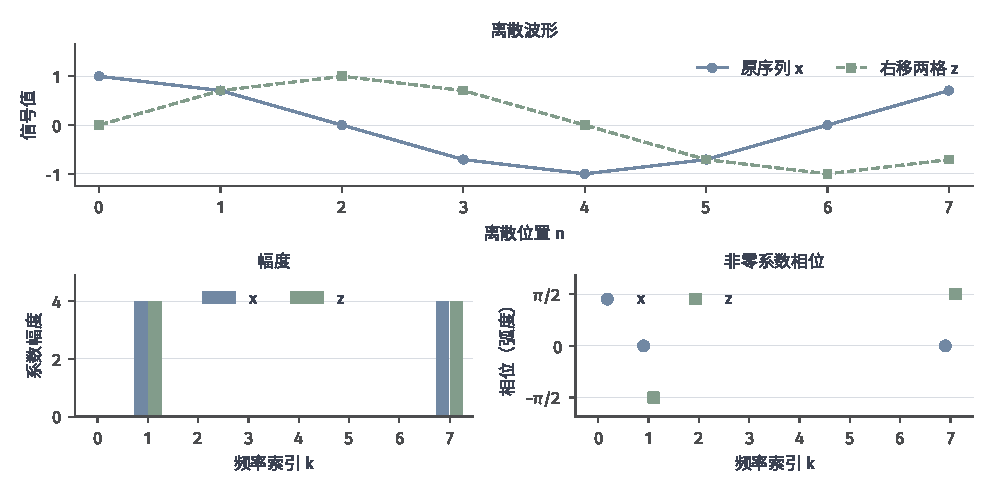
\includegraphics[width=169.0mm]{figures/01-mathematical-preliminaries-upper/07-signals/matplotlib/signal-amplitude-phase/figure.pdf}
  \caption{长度$8$的教学信号$x[n]=\cos(2\pi n/8)$及其循环延迟两格的结果。
  上方波形的峰值位置不同，下方在$k=1,7$的幅度均为$4$，相位却发生改变。
  相位图只画非零系数；波形连线只用于帮助观察顺序，并不表示已选择某种连续时间插值。}
  \label{fig:signal-amplitude-phase}
\end{figure*}

这里的复指数坐标来自规则的循环平移：每次移动都有统一的方向和步长，DFT同时分解这些平移。
如果位置之间只通过不规则的连接发生关联，就不能再凭编号判断谁是“下一格”。
第~\ref{sec:signal-analysis-graph-state-kernels}节将改用图上的连接来定义变化，
并通过环图说明这里的复指数如何成为图谱的一个特例。

\subsubsection{周期连续信号的傅里叶表示}

连续时间的一个周期含有无穷多个位置，有限个坐标一般不足以完整描述它。
周期条件仍然把频率限制在整数谐波上，但展开随之变成无穷级数。
\begin{definition}[周期信号的傅里叶系数与级数]
  \label{def:signal-analysis-fourier-series}
  设$T>0$，$f\in L^2[0,T]$并按周期$T$延拓。在内积
  \[
    \langle f,g\rangle_T=\frac1T\int_0^T \overline{f(t)}g(t)\,\mathrm dt
  \]
  下，复指数$e^{\mathrm i2\pi kt/T}$组成一组正交归一基。
  \term{傅里叶系数}（Fourier coefficient）为
  \[
    c_k=\frac1T\int_0^T f(t)e^{-\mathrm i2\pi kt/T}\,\mathrm dt,
    \qquad k\in\mathbb Z,
  \]
  即$c_k=\langle e^{\mathrm i2\pi k(\cdot)/T},f\rangle_T$：先固定基方向，再读取$f$的系数。
  相应的傅里叶级数写作
  \begin{equation}
    f(t)\sim\sum_{k\in\mathbb Z}c_ke^{\mathrm i2\pi kt/T}.
    \label{eq:signal-analysis-fourier-series}
  \end{equation}
\end{definition}
这里直接使用周期复指数系在$L^2[0,T]$中完备这一标准结论，其证明不在本节展开。
正交性由对$e^{\mathrm i2\pi(k-j)t/T}$积分得到：$k=j$时归一化积分为$1$，
否则两个端点的指数相同，积分为$0$。完备性给出对称部分和
$S_Kf=\sum_{|k|\leq K}c_ke^{\mathrm i2\pi kt/T}$的$L^2$收敛，
即$T^{-1}\int_0^T|S_Kf-f|^2\to0$。它描述一个周期上的平均平方误差，
不能仅凭这一结论就在每个$t$处写逐点等号。

由正交展开及其极限得到
\begin{equation}
  \frac1T\int_0^T|f(t)|^2\,\mathrm dt
  =\sum_{k\in\mathbb Z}|c_k|^2.
  \label{eq:signal-analysis-continuous-parseval}
\end{equation}
左边是一个周期上平均的幅值平方，后面将用它定义周期信号的平均功率。
若要计算一个周期的平方积分，还需再乘以$T$；非零周期信号在整条实轴上的平方积分则为无穷。
相应的截断误差为$\sum_{|k|>K}|c_k|^2$。
实信号满足$c_{-k}=\overline{c_k}$，延迟$\tau$则把$c_k$变为
$e^{-\mathrm i2\pi k\tau/T}c_k$，幅度与相位的作用和有限情形相同。

逐点重构需要附加更强的规则性。例如在一个周期内分段$C^1$、只有有限个跳跃点
且单侧极限存在时，傅里叶级数在连续点趋于$f(t)$，在跳跃点趋于左右极限的平均值。
这是带条件的结论；不能把均方收敛与逐点收敛或一致收敛混为一谈。
逐点收敛与一致收敛的区别见第~\ref{chap:limits-continuity}章，
均方误差所用的积分范数见第~\ref{chap:functional-analysis-and-approximation}章。

取周期$2\pi$的方波：$0<t<\pi$时为$1$，$-\pi<t<0$时为$-1$。
其平均值$c_0=0$；对$k\neq0$直接积分，
\[
  c_k=\frac1{2\pi}\left(
    \int_0^\pi e^{-\mathrm ikt}\,\mathrm dt
    -\int_{-\pi}^0 e^{-\mathrm ikt}\,\mathrm dt\right)
  =\frac{1-(-1)^k}{\pi\mathrm ik}.
\]
因此偶数$k$的系数为零，奇数$k$的系数为$2/(\pi\mathrm ik)$，也可配对写成
\[
  \frac4\pi\left(\sin t+\frac{\sin3t}{3}+\frac{\sin5t}{5}+\cdots\right).
\]
在连续点恢复$\pm1$，在跳跃点趋于$0$；无论给原函数的跳跃点赋什么值，
其$L^2$元素和傅里叶系数都不变。Parseval还给出
$1=(8/\pi^2)\sum_{j=0}^{\infty}(2j+1)^{-2}$。
平均平方误差趋于零并不排除跳跃附近的局部振荡；这正是用有限谐波逼近尖锐边沿时，
需要单独观察局部误差的原因。

\subsubsection{整轴离散信号的傅里叶表示}

一条整轴上的序列不必周期，频率也不再局限于$N$个格点。
但整数$n$使$e^{-\mathrm i(\omega+2\pi)n}=e^{-\mathrm i\omega n}$，
所以频率变量虽然连续，频率表示仍以$2\pi$为周期。
\begin{definition}[离散时间傅里叶变换]
  \label{def:signal-analysis-dtft}
  对$x\in\ell_1(\mathbb Z)$，即$\sum_{n\in\mathbb Z}|x[n]|<\infty$的序列，
  \term{离散时间傅里叶变换}（discrete-time Fourier transform, DTFT）定义为
  \begin{equation}
    X(e^{\mathrm i\omega})=\sum_{n\in\mathbb Z}x[n]e^{-\mathrm i\omega n},
    \qquad \omega\in\mathbb R.
    \label{eq:signal-analysis-dtft}
  \end{equation}
  绝对可和使级数绝对且一致收敛，因而定义出一个连续的$2\pi$周期函数。
\end{definition}
记号$X(e^{\mathrm i\omega})$强调只沿单位圆取值，这里不假设存在关于一般复变量的解析延拓。
对$x\in\ell_2$，同一个级数改按$L^2([-\pi,\pi])$收敛来理解，
所得对象是一个等价类，不要求每个$\omega$都能按普通级数求值。
两种情形都有系数恢复公式和能量关系
\begin{align*}
  x[n]&=\frac1{2\pi}\int_{-\pi}^{\pi}
  X(e^{\mathrm i\omega})e^{\mathrm i\omega n}\,\mathrm d\omega,\\
  \sum_n|x[n]|^2&=\frac1{2\pi}\int_{-\pi}^{\pi}|X(e^{\mathrm i\omega})|^2\,\mathrm d\omega.
\end{align*}
在$\ell_1$情形，可以把绝对收敛的级数移入积分，单位复指数的正交性只留下第$n$项；
$\ell_2$情形则来自周期$L^2$空间的正交基与Parseval关系。

贯穿例零延拓后的DTFT是
$X(e^{\mathrm i\omega})=1+2e^{-\mathrm i\omega}+e^{-2\mathrm i\omega}$，
它是一条连续频率曲线。对$N\geq3$，把记录补零到$N$项后再算DFT，
只是读取这条曲线在$\omega=2\pi k/N$处的值。补更多的零提高了频率格的密度，
却没有增加原记录的信息，也没有延长真实观测。
反过来，若原序列无穷长，先截取$N$项再作DFT，频谱已经受到时间截断的影响，
不能把结果直接称为完整DTFT的精确采样。
离散频率$\omega$的单位是弧度每样本；只有当样本间隔为$T_s$时，才换算成
连续角频率$\Omega=\omega/T_s$，并保留模$2\pi/T_s$的歧义。

\subsubsection{整轴连续信号的傅里叶表示}

最后一种情形最自由：信号定义在整条时间轴上，既没有有限长度，也不预设周期，
于是频率可取任意实数，离散的求和也变成对频率的积分。这里要留意一个严谨性的分界：
要求积分绝对存在（$L^1$）足以定义变换，但要在“能量有限”（$L^2$）的一般信号上使用，
还需要一次延拓，二者的依据并不相同。下面先在$L^1$上给出变换，再说明如何延拓。
\begin{definition}[连续时间傅里叶变换]
  \label{def:signal-analysis-continuous-fourier-transform}
  对$f\in L^1(\mathbb R)$，连续时间傅里叶变换为
  \[
    F(\Omega)=\int_{\mathbb R}f(t)e^{-\mathrm i\Omega t}\,\mathrm dt.
  \]
  若还满足$F\in L^1$，逆变换
  \[
    f(t)=\frac1{2\pi}\int_{\mathbb R}F(\Omega)e^{\mathrm i\Omega t}\,\mathrm d\Omega
  \]
  在几乎处处意义下成立，右侧给出一个连续代表元；在原$f$的连续点也恢复其点值。
  在$L^1\cap L^2$上使用同一积分公式，Plancherel定理把变换唯一延拓到$L^2$，满足
  \[
    \int_{\mathbb R}|f(t)|^2\,\mathrm dt
    =\frac1{2\pi}\int_{\mathbb R}|F(\Omega)|^2\,\mathrm d\Omega.
  \]
\end{definition}
一般$L^2$情形的正、逆变换按范数极限理解，不保证普通积分在每个频率或每个时刻都存在。
例如改变单个点的值不会改变$L^2$元素，变换不可能判断这个点后来被赋成了哪个值。
第~\ref{sec:signal-bandlimited-recovery}节将借助带限条件先选定连续代表元，
然后才读取采样点；不能对任意等价类未经说明就直接采样。

一个可以直接积分的例子是$f=\mathbb I_{[0,1]}$：
\[
  F(\Omega)=
  \begin{cases}
    (1-e^{-\mathrm i\Omega})/(\mathrm i\Omega),&\Omega\neq0,\\
    1,&\Omega=0.
  \end{cases}
\]
时域函数$f$在$[0,1]$之外取零，频谱$F$在任意大的频率之外却仍可能非零。
时间范围有限推不出频率范围有限。后面采样重构所需的带限条件约束的是频谱支撑，
必须另行核对。对满足积分条件的实信号，$F(-\Omega)=\overline{F(\Omega)}$；
延迟$\tau$使频谱乘上$e^{-\mathrm i\Omega\tau}$，仍然只改相位、不改幅度。
这里$\Omega$以弧度每单位时间计，不能与DFT中无量纲的索引$k$直接比较。

表~\ref{tab:reader-fourier-objects}汇总四种对象。它们的共同点是复指数坐标，
差别来自索引和周期条件，而不是四个名称可以互换。
\begin{table*}[htbp]
  \centering
  \begin{tabularx}{\linewidth}{lXXX}
    \toprule
    表示 & 输入对象及边界 & 频率坐标 & 成立口径\\
    \midrule
    DFT & $N$项数组，基采用循环索引 & $N$个频率格 & 有限和，可逆\\
    傅里叶级数 & 一个周期上的函数 & 全部整数谐波 & $L^2$均方展开；逐点另需条件\\
    DTFT & 整数轴序列，不要求周期 & 连续且$2\pi$周期 & $\ell_1$下连续；$\ell_2$下为$L^2$等价类\\
    连续傅里叶变换 & 实轴函数，不要求周期 & 连续实频率 & $L^1$积分或$L^2$延拓\\
    \bottomrule
  \end{tabularx}
  \caption{信号对象决定傅里叶表示的频率轴及收敛意义。离散时间不表示频率必然离散，
  频谱周期也不表示原序列周期；有限DFT与整轴DTFT之间还相差记录范围和边界约定。}
  \label{tab:reader-fourier-objects}
\end{table*}

\subsubsection{多维信号的傅里叶表示}
\label{sec:signal-multidimensional-fourier}

一维频率只用一个数就能说明“每隔几格重复一次”，图像却有行、列两个方向，一个数不够用了：
同一张灰度图上，可能沿横向每隔四格出现一道竖条纹，沿纵向却每隔两格就重复一次，
两个方向的快慢必须分别记录。也不能把图像拉平成一条首尾相接的长序列，
否则“向右挪一格”和“向下挪一格”会被当成同一种平移，条纹朝哪个方向延伸也就看不出来了。

先看一个能同时描述两个方向的具体模式：
\[
  \phi_{u,v}[n_1,n_2]=e^{2\pi\mathrm i(un_1+vn_2)}.
\]
沿列方向（$n_1$增加）它的频率是$u$，沿行方向（$n_2$增加）是$v$。
例如$u=1/4$、$v=0$给出每隔四列重复的竖条纹，$u=0$、$v=1/4$给出每隔四行重复的
横条纹，两个数都非零则得到斜条纹。它写成两个一维复指数相乘，
不过是利用指数相加把两个方向的相位叠在一起：
$e^{2\pi\mathrm iun_1}e^{2\pi\mathrm ivn_2}=e^{2\pi\mathrm i(un_1+vn_2)}$，
并没有新的运算。下面就用这一族模式给整张图建立一组坐标，
逆变换和能量关系则分别在两个方向各用一次单位根正交性。

\paragraph{规则网格上的频率坐标}
设$N_1,N_2$为正整数，$x[n_1,n_2]$定义在$0\leq n_1<N_1$、$0\leq n_2<N_2$。
两个坐标分别循环延拓，记$P=N_1N_2$，定义
\begin{equation}
 \begin{aligned}
 X[k_1,k_2]
 &=\sum_{n_1=0}^{N_1-1}\sum_{n_2=0}^{N_2-1}
 x[n_1,n_2]\\
 &\qquad\cdot e^{-2\pi\mathrm i(k_1n_1/N_1+k_2n_2/N_2)},\\
 x[n_1,n_2]
 &=\frac1P\sum_{k_1=0}^{N_1-1}\sum_{k_2=0}^{N_2-1}
 X[k_1,k_2]\\
 &\qquad\cdot e^{2\pi\mathrm i(k_1n_1/N_1+k_2n_2/N_2)}.
 \end{aligned}
 \label{eq:signal-multidimensional-dft}
\end{equation}
把第一式代入第二式，每个坐标上的单位根之和分别消去不相同的位置；
只有两个坐标都相同时才留下因子$N_1N_2$，因此恢复原值。
同样的正交关系给出
$\sum_{\bm n}|x[\bm n]|^2=P^{-1}\sum_{\bm k}|X[\bm k]|^2$。
取$N_1=N_2=2$及
$\bm x=\begin{bmatrix}1&2\\3&4\end{bmatrix}$，
可算得$\bm X=\begin{bmatrix}10&-2\\-4&0\end{bmatrix}$；
两侧能量分别为$30$与$(100+4+16)/4=30$。

双重有限和可以先沿$n_2$求和、再沿$n_1$求和。
所以逐行再逐列作一维DFT就是同一个变换；使用FFT时，代价为
$O(P(\log N_1+\log N_2))$，但要额外容纳中间数组。
这也说明一般$d$维网格为何使用各轴复指数的乘积，而不是另造一套一维编号。

把这套坐标用在一张真实灰度照片上，可以非常直观地看清“低频、高频”分别对应画面里的什么。
图~\ref{fig:real-image-spectrum}左是一张由天空、山坡、房屋和树组成的画面：天空的渐变、山坡的起伏
都很平缓，能量集中在频谱中央（低频）；屋檐、门窗、树干这些亮度突变的边缘朝各个方向伸展，
能量沿外围放射状分布（高频）。因此二维频率不是抽象编号——中央有多亮大致决定整体明暗，
外围哪些方向有能量，就说明画面里有朝哪些方向的边缘。
\begin{figure*}[htbp]
  \centering
  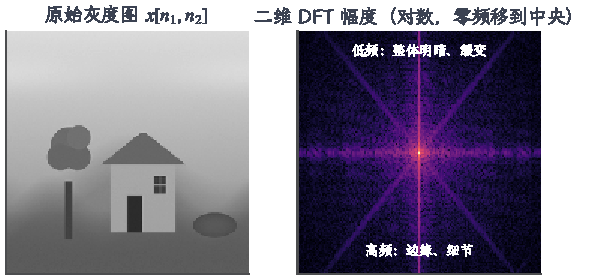
\includegraphics[width=0.92\textwidth]{figures/01-mathematical-preliminaries-upper/07-signals/matplotlib/teaching-signals-real-image/real-image-spectrum.pdf}
  \caption{同一张灰度照片（左）与其二维DFT幅度（右，取对数并把零频移到中央）。
  天空渐变、山坡等缓变区域对应中央附近的低频；屋檐、门窗、树干等亮度突变的边缘
  对应外围高频，且边缘朝哪个方向延伸，频谱就沿其法向出现能量。
  画面由确定性脚本生成，用于教学演示。}
  \label{fig:real-image-spectrum}
\end{figure*}

\paragraph{方向、平移与实值对称}
模式$\phi_{u,v}$的条纹方向可以直接从相位看出：沿与向量$(u,v)$垂直的方向走，
括号里的$un_1+vn_2$不变，整个复指数的值也不变，所以条纹沿垂直方向延伸；
换句话说，频率向量$(u,v)$指向的是条纹的法向，其模长表示沿法向每单位位置振荡多少次。
还是前面的例子：$u=1/4$、$v=0$时条纹竖直延伸（横方向上每四格一道），
而$u=v=1/4$给出斜条纹，不能简单说它“横竖各振荡四格”。
整数网格上每个方向的频率都按模$1$辨认，所以不能把任意大的频率模长都解释成更快、
还能被分辨的振荡——它会折回$[-1/2,1/2]$，这就是网格上的摩尔纹来源。
循环平移$\bm r=(r_1,r_2)$使频率系数乘上
$e^{-2\pi\mathrm i(k_1r_1/N_1+k_2r_2/N_2)}$；
实值输入满足
$X[(-k_1)\bmod N_1,(-k_2)\bmod N_2]=\overline{X[k_1,k_2]}$。
两式分别由位置换元和取共轭得到，幅度、相位和自共轭格点的含义沿用一维结论。
特别地，当两个边长都是偶数时，把每个像素的读数乘上$(-1)^{n_1+n_2}$
（即相邻像素正负交替，像棋盘格）正好把频谱沿两个方向各平移半个周期；
边长为奇数时整数频率格里没有对应的半个格点，这一操作就不是精确的半周置换。

\paragraph{连续坐标改变下的频谱}
把网格换成连续平面，就得到多维连续傅里叶变换。对$f\in L^1(\mathbb R^d)$，令
$F(\bm\Omega)=\int_{\mathbb R^d}f(\bm t)e^{-\mathrm i\bm\Omega^\top\bm t}\,
\mathrm d\bm t$，绝对可积保证积分存在。
若$F$也绝对可积，系数为$(2\pi)^{-d}$的逆积分几乎处处恢复$f$，并给出连续代表元；
$L^2$延拓下的能量关系使用同一系数。

这条公式的用处在于：当我们把图像放大、缩小或旋转时，可以直接看出频谱怎样跟着变，
而不必重新逐点推导。现在改变坐标、但不改变函数的取值规则：对可逆实矩阵$\bm A$和向量$\bm b$，
令$g(\bm t)=f(\bm A\bm t-\bm b)$，其中$\bm A$负责旋转、拉伸等坐标变换，$\bm b$负责平移。
换元$\bm u=\bm A\bm t-\bm b$得到
\begin{equation}
 G(\bm\Omega)=|\det\bm A|^{-1}
 e^{-\mathrm i\bm\Omega^\top\bm A^{-1}\bm b}
 F(\bm A^{-\top}\bm\Omega).
 \label{eq:signal-fourier-coordinate-change}
\end{equation}
行列式来自体积改变，逆转置来自相位的线性配对。这条公式不要求记住矩阵形式，
只要抓住“空间和频率此消彼长”：把图像在空间里放大$a$倍，
频谱反而被压缩到原来的$1/a$。具体地，$g(\bm t)=f(\bm t/a)$、$a>0$使对象扩大$a$倍，
其频谱为$a^dF(a\bm\Omega)$，频率范围反而缩小；$f(a\bm t)$则给出$a^{-d}F(\bm\Omega/a)$。
直观上，放大图像会让一道条纹占据更宽的空间距离，所以它每单位长度振荡的次数变少。
连续旋转的公式是精确恒等式，但有限像素网格上旋转任意角度后还要把新位置的读数
由周围像素插值得到、并处理越界边界，不能把重采样误差藏进这条恒等式。

\subsubsection{反射边界下的余弦表示}
\label{sec:signal-cosine-representation}

前面做DFT时默认把有限记录首尾相接。这要求记录的最后一个读数和第一个读数本来就接近，
否则连接处会出现一次记录里并不存在的突变。举个最小的例子，$x=(1,2,3)$首尾相差$2$，
首尾相接后从$3$突然掉到$1$，频谱里就多出一大批表示这次“假跳变”的高频系数；
而这些高频并不是原记录的内容，只是我们强加的连接方式造成的。
若问题本身适合让信号在边界处折返而不是硬接（例如一段关于对称位置的测量），
可以先把记录对折叠长、再在折叠后的周期记录上使用已有的复指数坐标。
这样连接处两边的值相同，就不会凭空产生跳变。
这里要弄清三件事：镜像位置怎样决定相位，怎样归一化才能保持能量，
以及用小整数近似余弦权重时，它的尺度为何必须与逆变换一起处理。

\paragraph{镜像延拓与余弦系数}
先看镜像具体怎么折。对实记录$x[0],\ldots,x[N-1]$，在每个原始读数旁边放上它的镜像：
前半段照抄$x[0],\ldots,x[N-1]$，后半段倒序再写一遍，使位置$n$与位置$2N-1-n$读到同一个值。
用公式写就是构造长度$2N$的序列
$y[n]=x[n]$（$0\leq n<N$）、
$y[2N-1-n]=x[n]$。
注意折返发生在最末端读数之后的那个“半格”上，所以最后一个值$x[N-1]$在序列中出现两次
（开头还有一份$x[0]$），端点重复；它与前述不重复端点的反射约定不同。
把这两份相同读数在$2N$点DFT中配成一对，一个配$e^{+\mathrm i\theta}$、
另一个配$e^{-\mathrm i\theta}$，相加后虚部抵消、只剩余弦，得到
\[
 Y[k]=2e^{\mathrm i\pi k/(2N)}
 \sum_{n=0}^{N-1}x[n]\cos\frac{\pi k(n+1/2)}N .
\]
前面的相位$e^{\mathrm i\pi k/(2N)}$是已知的，去掉它就只剩实数系数。
\term{第二类离散余弦变换}（type-II discrete cosine transform, DCT-II）采用正交归一形式
\begin{equation}
 \begin{aligned}
 c_k&=\alpha_k\sum_{n=0}^{N-1}x[n]
 \cos\frac{\pi k(n+1/2)}N,\\
 \alpha_0&=N^{-1/2},\qquad \alpha_k=(2/N)^{1/2}\ (k>0).
 \end{aligned}
 \label{eq:signal-dct-two}
\end{equation}
设矩阵$\bm C$的第$(k,n)$项就是式中的余弦权重。
积化和差与有限几何和给出：两条不同余弦行的内积为零，
常数行的平方和为$N$，其余行的平方和为$N/2$。
具体地，交叉项化成
$\sum_{n=0}^{N-1}\cos(\pi r(n+1/2)/N)$；
对$1\leq r<2N$该和为$\sin(\pi r)/(2\sin(\pi r/(2N)))=0$。
因此$\bm C\bm C^\top=\bm I$，逆变换是$\bm x=\bm C^\top\bm c$，
且$\|\bm x\|_2^2=\|\bm c\|_2^2$。
$N=2$、$\bm x=(1,3)^\top$给出$\bm c=(2\sqrt2,-\sqrt2)^\top$；
第一项读取平均水平，第二项读取差异，平方和仍是$10$。

\paragraph{二维表示与整数近似}
对一张$N_1\times N_2$的图像（即一个矩形数组$\bm X$），DCT可以沿两个方向各做一次：
先把每一列按长度$N_1$的余弦基展开，再把每一行按长度$N_2$展开。用矩阵写，
正向变换为$\bm Y=\bm C_{N_1}\bm X\bm C_{N_2}^\top$，
逆变换为$\bm X=\bm C_{N_1}^\top\bm Y\bm C_{N_2}$，Frobenius范数保持不变。
保留部分系数时，重建误差的平方恰是舍弃系数的平方和——这与一维截断完全对应，
只是现在“低频”指两个方向上的余弦波数都小。
常数数组只留下常数系数；一幅整体缓变的图像通常能把较多能量放在低阶系数，
但任意输入都可以取成某条高阶基向量，所以不存在无条件的低频能量集中保证。
图~\ref{fig:real-image-dct}给出这一“能量集中”在真实画面上的效果：只保留左上角
$64\times64$个低频系数（约占全部$6.2\%$）就重建出房屋的整体轮廓和明暗，
但门窗格子、树叶等细节都模糊了——压缩时正是据此丢弃大量接近零的高频系数。
\begin{figure*}[htbp]
  \centering
  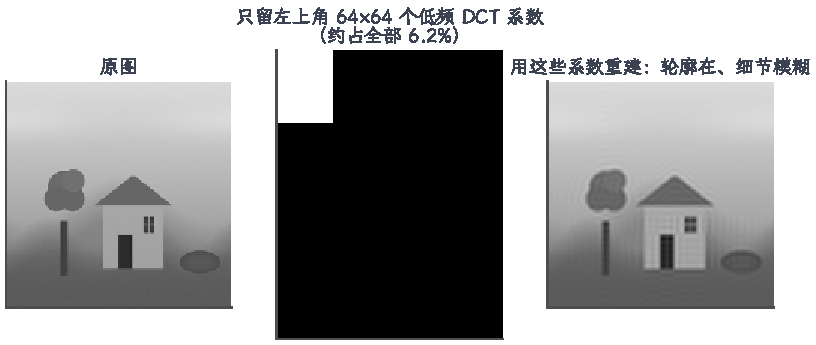
\includegraphics[width=0.95\textwidth]{figures/01-mathematical-preliminaries-upper/07-signals/matplotlib/teaching-signals-real-image/real-image-dct.pdf}
  \caption{二维DCT的低频能量集中。仅保留左上角$64\times64$个低频系数（中），
  仍能重建出房屋轮廓与整体明暗（右），但高频细节缺失、画面模糊；
  这正是JPEG等压缩舍弃高波数系数的依据。教学画面由脚本确定性生成。}
  \label{fig:real-image-dct}
\end{figure*}

若用小整数矩阵$\bm T$近似这些余弦行，必须重新检查$\bm T\bm T^\top$。
当它等于正对角矩阵$\bm D$时，$\bm D^{-1/2}\bm T$才正交，
而未归一化读数$\bm y=\bm T\bm x$的精确逆为
$\bm x=\bm T^\top\bm D^{-1}\bm y$。
例如$\bm T=\begin{bmatrix}1&1\\1&-1\end{bmatrix}$满足$\bm D=2\bm I$，
逆式中含有$1/2$。逐行缩放可以并入后续量化步长，却不能在解码时丢掉。
若行之间仍有非零内积，除以行长并不能使它们正交；
取整与溢出还会另添误差，整数运算本身不保证有损编码逐位可逆。

\subsubsection{局部片段的时频表示}
\label{sec:signal-local-frequency}

整段DFT回答了“记录里有哪些频率”，却丢掉了“这个频率在什么时候出现”。
最典型的是一段录音：前半段是低音、后半段才响起一声高音，但DFT只会告诉你
“低音和高音都存在”，无法说出高音是在第几秒才进来的。要同时保留时间和频率，
办法是用一个固定长度的小窗口沿记录滑动，每次只看窗口内的一小段、对这一小段作DFT；
窗口移到不同位置，就得到不同时刻的局部频谱。下面的短时傅里叶变换正是这样做的。
这里有一个无法两全的取舍：窗口越短，越能说清某个频率“在什么时候”，
但窗口里装下的周期越少，能分辨的频率就越粗；反之亦然。
困难还在于片段两端被突然截断会改变频谱。
下面先固定分帧公式，再从有限和看待这种泄漏，最后说明频率读数怎样合并成新的坐标。

\paragraph{窗口、帧移与频率泄漏}
先把操作说具体：选一个长度$N$的小窗$w[n]$（最简单就是窗内全取$1$，即只截取、不额外加权），
再让它每次向右移动$H$格。窗口每停在一个起始位置$mH$，就把这$N$个读数乘上窗权、作一次DFT。
\term{短时傅里叶变换}（short-time Fourier transform, STFT）为
\begin{equation}
 S[m,k]=\sum_{n=0}^{N-1}x[mH+n]w[n]e^{-2\pi\mathrm i kn/N}.
 \label{eq:signal-stft}
\end{equation}
对有限记录还要另给补边规则，或舍弃不完整的帧。
帧$m$的位置由$mH$确定；若采样率为$f_s$，窗口时长为$N/f_s$，
DFT格点间隔为$f_s/N$。这些格点间距并不自动等于分辨两个邻近分量的能力，
后者还取决于窗口主瓣宽度和分量幅度。

设某帧未加窗的$N$点DFT为$X_m$、窗口的DFT为$W$。
代入逆变换并交换有限和可得
$S[m,k]=N^{-1}\sum_\ell X_m[\ell]W[(k-\ell)\bmod N]$。
时间上相乘变成频率上循环卷积，窗口会把一个频率的贡献铺到附近位置。
即使矩形窗口在窗口内恒为一，被截取的整轴复指数
$e^{\mathrm i\omega_0 n}$若不落在DFT格点上，也给出
\[
 S[k]=e^{\mathrm i(N-1)\delta/2}
 \frac{\sin(N\delta/2)}{\sin(\delta/2)},\qquad
 \delta=\omega_0-2\pi k/N,
\]
分母为零时按连续极限取$N$。
一个频率的能量散到多个格点、在旁边留下非零读数，称为\term{频谱泄漏}（spectral leakage）。
它的根源正是窗口两端的突然截断：无限延续的正弦只有一个频率，被硬切成有限一段后，
就像给这段正弦又乘了一个“矩形开关”，而这个开关自己含有大量频率，二者的频率混在一起。
例如$N=4$、$\omega_0=\pi/4$时，
$k=0,1$的模长都是$1/\sin(\pi/8)$，不能只把最大格点当作原来的单频。
补救方法是让窗口两端平缓地降到零（即渐消窗口），这样可以压低远处那些小的旁瓣，
但窗口等价于被进一步缩短，通常会把中央的主瓣撑宽，附近频率更难分开。
还要注意，在记录后面补零只是把同一窗口的频率曲线采得更密，
让频率图画得更平滑，并不能补回被截掉的时间信息、也提高不了真实分辨能力。

\paragraph{功率读数与频带汇总}
谱图常显示$|S[m,k]|$或$|S[m,k]|^2$，必须说明用的是哪一个以及如何归一化。
实信号每帧有共轭对称性，保留$0\leq k\leq\lfloor N/2\rfloor$就足以表达该帧；
但计算全谱能量时，非自共轭格点的贡献仍要成对计入。
给定非负权重$B_{b,k}$，频带读数可写成
$E[m,b]=\sum_k B_{b,k}|S[m,k]|^2$。
对功率数组而言这是线性加权，对原信号则不是线性映射。
例如\term{梅尔频率}（mel frequency）常用
$\mu(f)=2595\log_{10}(1+f/700)$，并在此坐标上等距放置三角形权重；
它是一种频率刻度与权重设计，并不改变DFT定理。
再取$\log(E+\varepsilon)$需给出$\varepsilon>0$，并引入进一步的非线性。
只保存功率或频带和，一般无法恢复每帧的相位。

\subsection{有限信号的多项式表示}
\label{sec:signal-analysis-polynomial-arithmetic}

对于有限序列，还可以用多项式的幂次记录位置、用系数记录各位置的读数。
具体做法只是“给每个位置配一个不同次数的$z$”：位置$0$的读数配$z^0$，
位置$1$配$z^1$，以此类推，整条数组就变成一个多项式。
这种“把数组看成多项式”的做法初看像记号游戏，但它提供了第三套坐标，
而且很快会带来一个实实在在的好处——多项式乘法在合并同类项$z^n$时，
恰好是把“所有位置之和为$n$的乘积”加在一起，这正是卷积定义里要做的同一件事。
把数组写成多项式，承接了第~\ref{chap:linear-algebra-and-matrix-analysis}章
把多项式视为向量的做法；本节先建立求值、插值与取余之间的恢复关系，
卷积快速计算那一节再用这些表示减少乘法次数。
由此得到的多项式可以换成点值坐标或余数坐标，不过要恢复全部系数、
所需信息量取决于次数界和所选坐标。这里先弄清什么时候可以恢复。

\subsubsection{基于位置系数的多项式表示}

对$\bm x=(x_0,\ldots,x_{m-1})$定义
\[
  X(z)=\sum_{j=0}^{m-1}x_jz^j.
\]
其中$x_j=x[j]$，形式变量$z$首先只用来记录位置，并不是施加给系统的输入。
长度固定之后，序列与次数小于$m$的多项式一一对应；最高位置的系数可以为零，
所以次数未必恰好是$m-1$。例如贯穿记录与核分别对应
$X(z)=1+2z+z^2$和$H(z)=1-z$。
移动一个位置并保留前导零对应乘以$z$：$1+2z+z^2$乘$z$后各项次数都加一，
读数整体后移一格。至于是否把超出的最高次项回绕到低次项（循环边界），
仍要由边界另行规定。还有一层联系值得先记住：DFT的正变换正是把$X$在单位根$\omega_N^k$处
逐一求值。所以多项式在这里把“位置系数”和“频率系数”连成同一对象的两种坐标，
并没有改变记录本身。

\subsubsection{基于互异点值的插值表示}

已知一个多项式在若干位置的值，什么时候足以恢复全部系数？
先建立一个直观事实：两点只能确定一条直线，三点（且知道它至多是二次）才能确定一条抛物线；
所以点数和“最高允许到几次”必须搭配。次数小于$L$的多项式构成$L$维空间，
在$L$个两两不同的点上各取一个值，恰好给出$L$个独立条件。
选取$L$个两两不同的点$a_0,\ldots,a_{L-1}$，求值映射
\[
  E(P)=(P(a_0),\ldots,P(a_{L-1}))
\]
是线性的。若$E(P)=0$，说明$P$在这$L$个不同点上都取零，即有$L$个不同的根；
但次数小于$L$的非零多项式至多有$L-1$个根，因此只能有$P=0$。
同维空间之间的单射必为双射，其逆映射就是\term{多项式插值}（polynomial interpolation）：
只要点够、又事先限定了最高次数，系数就能由这组点值唯一还原。

显式恢复可用Lagrange基
\[
  \ell_j(z)=\prod_{\substack{0\leq k<L\\k\neq j}}
  \frac{z-a_k}{a_j-a_k}.
\]
互异性保证分母非零，且$\ell_j(a_k)=\delta_{j,k}$。
所以$P$与下式右侧在$L$个点上相同、次数都小于$L$，由刚才的唯一性得到
\begin{equation}
  P(z)=\sum_{j=0}^{L-1}P(a_j)\ell_j(z),\qquad\deg P<L.
  \label{eq:signal-analysis-lagrange-interpolation}
\end{equation}
例如一次多项式在$0,1$处的值为$1,3$，便恢复为$1(1-z)+3z=1+2z$。
若允许二次项，则$1+2z+c\,z(z-1)$对任意$c$都给出相同的两点值，
说明次数界不可省略。重复读取同一点也不增加独立约束；导数观测属于另一种插值问题。

代数可逆不等于数值稳定。点值到系数的矩阵逆可能放大测量或舍入误差，
选点相近或次数较高时尤其要检查条件数，相关判断回用
第~\ref{chap:matrix-analysis}章。单位根上的归一化DFT是条件良好的特殊选点，
一般实点并没有同样的保证。

\subsubsection{基于互素余数的模分解表示}

点值坐标用起来方便，但每个点值只保存一个数，且默认要在一条直线（一次多项式）上读取。
还可以保存另一种更小的“片段”：多项式除以一个低次多项式后剩下的余数。
这和整数除法是同一回事——$17$除以$5$商$3$余$2$，余数$2$比除数小、也更容易处理；
多项式带余除法得到的余数次数严格小于除式，需要的系数自然更少。
关键在于，只要选的几个“除式”彼此没有公共因子，几份余数合起来就能唯一拼回原多项式，
这正是下一条快速卷积路线（Winograd）要用的工具。为使这种说法有确定含义，
先建立除法与唯一性，以下用$F$表示系数域。
域（field）是一套遵守通常加乘运算律、可以加减乘除且非零元素都能作除数的数系；
第一次读只需把它想成熟悉的实数或复数即可，本节的例子就取$F=\mathbb R$或$\mathbb C$。
$F[z]$表示系数在$F$中的有限多项式全体，采用通常的多项式加法与乘法。
\begin{theorem}[多项式带余除法]
  \label{thm:signal-analysis-polynomial-division}
  设$A,M\in F[z]$且$M\neq0$，存在唯一的$Q,R\in F[z]$满足
  \[
    A=QM+R,\qquad\deg R<\deg M.
  \]
  约定零多项式的次数为$-\infty$。
\end{theorem}
\begin{proof}
  若$\deg A<\deg M$，取$Q=0,R=A$。否则设最高次项分别为
  $a_pz^p$与$m_qz^q$，$p\geq q$。域中$m_q$可逆，减去
  $(a_p/m_q)z^{p-q}M$就消掉最高次项。每一步次数严格下降，
  有限步后便得到次数小于$\deg M$的余数。

  若还有$A=Q'M+R'$，则$(Q-Q')M=R'-R$。左侧若非零，次数至少为$\deg M$；
  右侧若非零，次数小于$\deg M$，矛盾。因此两侧都为零，$Q=Q'$、$R=R'$。
\end{proof}

对非零$A,B$反复作带余除法，
\[
  A=Q_0B+R_1,\qquad B=Q_1R_1+R_2,\qquad\ldots
\]
非零余数的次数严格下降，过程必在有限步终止。
由$A=Q_0B+R_1$可见，$A,B$的公因式恰好是$B,R_1$的公因式；
逐步应用，最后一个非零除数（包括最初的$B$）首项归一化后就是
\term{最大公因式}（greatest common divisor）。
从最后一个等式向前回代，各余数与初始除数$B$都是$A,B$的多项式线性组合，得到
\begin{equation}
  U(z)A(z)+V(z)B(z)=\gcd(A,B).
  \label{eq:signal-analysis-polynomial-bezout}
\end{equation}
这是Bézout恒等式。互素表示最大公因式是非零常数，等价于存在$U,V$使左侧为$1$。
例如在$\mathbb R[z]$中，
\[
  z^2+1=(z+1)(z-1)+2,\qquad
  1=\tfrac12(z^2+1)-\tfrac12(z+1)(z-1).
\]
它既证明$z-1$与$z^2+1$互素，也提供了后面重构所需的逆元。

把余数记为$A\bmod M$，把相差$M$倍的多项式看成同一个
\term{剩余类}（residue class），记为$[A]_M$（这和整数按模$5$把$2$和$7$看成同一类完全类似）。
一个关键联系是：当除式取成一次式$M=z-a$时，余数是个常数，而且正好等于多项式在$a$点的值
——除法式在$z=a$处给出$A(z)=Q(z)(z-a)+A(a)$，余数就是$A(a)$。
所以“记录点值”其实是“记录关于一次模的余数”的特例；选用次数更高、彼此互素的模，
就能保存更丰富的片段信息。下面的\term{多项式中国剩余定理}
（polynomial Chinese remainder theorem）说明，互素模下的各份余数怎样共同确定原对象。
\begin{theorem}[多项式中国剩余定理]
  \label{thm:signal-analysis-polynomial-crt}
  设非恒定多项式$m_1,\ldots,m_s\in F[z]$两两互素，令$M=\prod_{j=1}^s m_j$。
  映射
  \[
    [A]_M\longmapsto([A]_{m_1},\ldots,[A]_{m_s})
  \]
  是环同构（ring isomorphism），即双射并且保持加法和乘法；
  余数类相加或相乘，都是先作多项式运算再对相应的模取余。
  因此全部余数唯一确定次数小于$\deg M$的代表元$A\bmod M$。
\end{theorem}
\begin{proof}
  若$A-B$是$M$的倍数，它也是各$m_j$的倍数，故映射不依赖代表元；
  取余还保持加法与乘法。若$A,B$的各个余数都相同，则每个$m_j$都整除$A-B$。
  为证明乘积也整除，先设互素的$a,b$都整除$q$，写$q=ac$。
  由$ua+vb=1$有$c=uac+vbc=uq+vbc$，所以$b$整除$c$，从而$ab$整除$q$。
  两两互素时，若某多项式分别与$a,b$互素，把对应Bézout等式相乘即可证明
  它与$ab$互素。反复使用前述整除结论，便有$M\mid(A-B)$，映射为单射。

  给定任意余数$r_j$，令$M_j=M/m_j$。互素性与Bézout恒等式给出
  $u_jM_j+v_jm_j=1$。因此$e_j=u_jM_j$关于$m_j$的余数是$1$，
  关于其他$m_k$的余数是$0$。取
  \[
    A=\sum_{j=1}^s r_je_j
  \]
  即具有全部指定余数，故映射满射。最后对$M$取余，带余除法给出唯一的、
  次数小于$\deg M$的代表元。
\end{proof}

互素性使各份信息能够独立拼合，次数界使模意义下的唯一性成为原多项式的唯一性。
例如知道$P\bmod z$和$P\bmod(z-1)$可以恢复一次多项式，却无法区分
$P$与$P+c\,z(z-1)$；反复使用同一个模更不会增加信息。
在模$z^N-1$下，$z^{N+s}$与$z^s$属于同一剩余类，因而高次系数按模$N$合并。
这条规则将用来编码循环边界，但此时还没有计算两个信号的乘积。
余数恢复如何减少卷积计算，留到第~\ref{sec:signal-analysis-fast-transforms}节。

\section{信号的比较}
\label{sec:signal-comparison}

不同坐标描述的是同一条信号，但要比较信号，还得先确定评价口径。
峰值、累计幅值和平方累计回答的是不同的大小问题；内积比较模式的方向；
长期平均功率则描述持续信号的平均强度。这些指标都必须在相同的位置范围
和通道单位下计算才有意义。

\subsection{信号的大小比较}

比较两条记录谁更大之前，先要确定比较的到底是什么。
这一步与第~\ref{chap:linear-algebra-and-matrix-analysis}章选择向量范数的情形完全一样：
不存在对所有任务都合适的唯一口径，每个数回答的是不同的物理问题。
若要约束设备的最大读数，可以看峰值；若要累计全部幅值，可以求绝对值之和；
平方和则让较大的读数占更高权重，适合把异常尖峰看得更重。
对离散标量信号，这三种口径对应
\[
  \|x\|_\infty=\sup_k|x[k]|,\qquad
  \|x\|_1=\sum_k|x[k]|,\qquad
  \|x\|_2=\left(\sum_k|x[k]|^2\right)^{1/2}.
\]
在有限记录上求和只取记录范围；在整轴上则要求相应总和有限。
记$\ell_1(\mathbb Z)$为绝对可和序列空间，$\ell_2(\mathbb Z)$为平方可和序列空间。
例如$x[k]=(k+1)^{-1}$在$k\geq0$时取此值、$k<0$时取零，
属于$\ell_2$却不属于$\ell_1$。所以可以定义能量的信号，未必能直接使用
绝对收敛的变换或卷积论证。

连续情形把和换成积分，得到$L^1$与$L^2$范数；$L^\infty$采用
$\operatorname*{ess\,sup}_t|x(t)|$，即忽略零测异常点之后的最小本质上界。
它不同于最大值：函数可能只趋近其上界而从未取到，也可能在单个点被赋任意大的值，
却仍代表同一个$L^\infty$元素。真实采样要读取点值，届时必须另行确定代表元。

对贯穿有限记录，$\|x\|_\infty=2$、$\|x\|_1=4$、$\|x\|_2=\sqrt6$。
重排位置不改变这三个数，却可以改变局部波形；范数并不是完整的形状描述。
多通道的二范数可按
$\|\bm x\|_2^2=\sum_k\|\bm x[k]\|_2^2$定义；
不同通道若具有不同单位，需要先换算或明确选取权重。下一小节用带权内积说明这种比较，
这里的欧氏范数约定所有通道已经使用相容的数值尺度。

\subsection{信号的相似性比较}

比较两条记录是否接近，需要决定哪些位置和通道参与比较。
因为两条信号可能整体轮廓接近、却在某些关键时刻错位，
也可能逐点差异不小但高频抖动互相抵消；不同的对齐与加权会给出不同的“相似度”。
沿用前面说明的第一变量共轭线性约定，对有限记录、平方可和序列与平方可积函数分别有
\begin{equation}
  \begin{aligned}
    \langle x,z\rangle_N&=\sum_{k=0}^{N-1}\overline{x[k]}z[k],\\
    \langle x,z\rangle_{\ell_2}&=\sum_{k\in\mathbb Z}\overline{x[k]}z[k],\\
    \langle x,z\rangle_{L^2}&=\int_{\mathbb R}\overline{x(t)}z(t)\,\mathrm dt.
  \end{aligned}
  \label{eq:signal-inner-products}
\end{equation}
后两式中的逐点乘积$\overline{x[k]}z[k]$与$\overline{x(t)}z(t)$
由Cauchy--Schwarz不等式分别保证绝对可和与绝对可积。
内积为零表示在当前比较口径下二者正交，它诱导的距离为$\|x-z\|_2$。
对非零信号作归一化，$\rho(x,z)=\langle x,z\rangle/(\|x\|_2\|z\|_2)$满足$|\rho|\leq1$；
实信号时它是夹角余弦，复信号时一般是复数，包含相对相位。
零信号没有这种归一化相似性，不能直接除以零。

例如$x=(1,2,1)$、$z=(1,0,-1)$满足$\langle x,z\rangle=0$，
但两者在位置$0$都有非零值。正交描述的是汇总贡献相互抵消，并不要求支撑互不相交。
若把$x$换成$2x$，归一化相似性仍是$1$，距离却是$\|x\|_2$；
这说明方向相同与数值接近是两个不同的判断。

多通道内积同时汇总位置与通道：
\[
  \langle\bm x,\bm z\rangle
  =\sum_k\sum_{c=1}^d \overline{x_c[k]}z_c[k].
\]
如果不同传感器的单位或重要性不同，可以明确选取正权重$w_c$，把每项乘以$w_c$。
更一般地，Hermitian正定矩阵$\bm W$给出
$\sum_k\bm x[k]^*\bm W\bm z[k]$，其中$*$表示共轭转置。
正定性使非零信号的自内积为正；仅半正定时某些非零通道组合可能被忽略。
改变权重可能改变正交关系和相似性排序，不能把它当作不影响结论的单位装饰。

\subsection{信号的能量与功率比较}

振幅和频率都非零的连续时间正弦波可以无限持续。尽管每个时刻的读数都有界，
把整条时间实轴上的幅值平方积分，结果仍会发散。
这正是必须区分能量与功率的实际原因：能量回答“整条信号累计了多少”，
对持续振荡必然无穷大，无法用来比较；功率回答“平均到单位时间有多强”，
除掉时长之后才有有限值。于是要分别研究总累计量和长时间窗口内的平均累计量，
它们对应信号能量与平均功率。
\begin{definition}[信号能量与平均功率]
  \label{def:signal-energy-power}
  离散及连续信号的能量分别为
  \[
    E_x=\sum_{k\in\mathbb Z}|x[k]|^2,\qquad
    E_x=\int_{\mathbb R}|x(t)|^2\,\mathrm dt.
  \]
  能量有限等价于属于相应的$\ell_2$或$L^2$空间，且$E_x=\|x\|_2^2$。
  长期平均功率在相应极限存在时定义为
  \begin{align*}
    P_x&=\lim_{K\to\infty}\frac1{2K+1}\sum_{k=-K}^K|x[k]|^2,\\
    P_x&=\lim_{R\to\infty}\frac1{2R}\int_{-R}^R|x(t)|^2\,\mathrm dt.
  \end{align*}
\end{definition}

这里以幅值平方定义信号指标；若要解释为物理能量或功率，还需要相应单位和系统系数。
窗口能量则只在声明的记录窗口内求和或积分。
之所以要区分这两者，是因为持续振荡的信号每个时刻读数有界，累计平方却随
时间线性增长、并不收敛。贯穿例零延拓后的能量为$6$；若按周期$3$延拓，
单周期能量仍是$6$，平均功率却是$6/3=2$，而整轴能量发散。
一般周期序列满足$P_x=N^{-1}\sum_{k=0}^{N-1}|x[k]|^2$，
局部平方可积的$T$周期函数满足$P_x=T^{-1}\int_0^T|x(t)|^2\,\mathrm dt$。
两式都可由把长窗口分成完整周期与长度有界的剩余段得到。

对实参数$A,\Omega,\varphi$且$A\neq0$、$\Omega\neq0$的正弦信号
$x(t)=A\cos(\Omega t+\varphi)$，利用$\cos^2 u=(1+\cos2u)/2$可得
一个周期的平方积分为$A^2T/2$，故$P_x=A^2/2$，而无限多个周期的累计能量为无穷。
反过来，有限能量信号的长期平均功率为零，因为平均的分子不超过总能量，分母却趋于无穷。
非周期有界信号未必有平均功率极限：例如按$|t|$把时间轴分成取值$0$和$1$的交替块，
选取各块长度，使此前全部块的总长度与新块长度之比趋于零，沿各块端点取对称窗口时，
平方平均就分别趋近$0$或$1$，因而没有极限。

前面的Parseval关系只是在另一组坐标下计算这里已经定义好的能量或周期平均功率。
其中出现的$N$、$T$或$2\pi$尺度因子来自变换和内积的归一化，
并不是同一条信号换了坐标后获得了更多能量。

\section{信号的运算与映射}
\label{sec:signal-operations-maps}

时域、频域和多项式坐标描述的都是同一条信号。这些表示讨论的是同一个对象，
接下来要问的是：对信号作一次操作之后，它的各种坐标怎样变化。
平移与反转改变位置，缩放与叠加改变读数或时间尺度；
把这些操作当作系统的输入输出规则之后，还要检验系统是否满足线性和平移不变。
三类映射将依次出现：输出只依赖一个位置的无记忆映射，
输出依赖整段历史但仍保持线性和平移不变的卷积映射，
以及权重随输入或时刻改变、因而不满足这两条性质的映射。
模板相关在形式上接近卷积，却是把一条信号与不同的局部片段作比较，因此单独讨论。
每项运算都要保留前一节约定的边界条件。
局部差分把卷积权重与导数近似联系起来，多尺度映射把平均和细节分开保存；
量化再限制可存储的幅度，集合形态映射则把加权求和改成邻域中的“存在”与“全部”判断。
后面分别检查它们的可逆性、误差或序关系，避免把所有局部操作都当成线性滤波。

\subsection{信号的平移与反转}

为避免对称波形掩盖方向上的差别，本节固定一个非对称三角脉冲：
\begin{equation}
  x(t)=
  \begin{cases}
    2t,&0\leq t\leq1,\\
    3-t,&1<t\leq3,\\
    0,&\text{其余位置}.
  \end{cases}
  \label{eq:signal-asymmetric-wave}
\end{equation}
它在$t=1$达到峰值$2$，上升历时$1$、下降历时$2$，
能量为$\int_0^1 4t^2\,\mathrm dt+\int_1^3(3-t)^2\,\mathrm dt=4$。
图~\ref{fig:signal-basic-operations}始终用它作参照。

\subsubsection{信号的平移}

连续时间延迟$\tau$写成$(T_\tau x)(t)=x(t-\tau)$；
离散时间沿用$(T_rx)[k]=x[k-r]$，只允许整数$r$。
正参数使已有特征推迟出现，负参数使其提前。
例如$x(t-1)$的峰值从$t=1$移到$t=2$，支撑从$[0,3]$移到$[1,4]$。
长度$N$的循环延迟则是$x[(k-r)\bmod N]$，越过右端的值回到左端。
对有限的非循环记录，必须先按第~\ref{sec:signal-objects-structure}节约定延拓，
再决定是否裁剪回原窗口，不能把丢出窗口的值自动送回首端。

对整轴上同一信号空间的$x,z$，换元给出
$\langle T_\tau x,T_\tau z\rangle=\langle x,z\rangle$；
离散情形用求和换标、循环情形用有限位置的置换得到相同结论。
相应的整轴$L^p$、$\ell_p$范数和能量都不变。
但在固定窗口$[0,3]$内，$x(t-1)$只保留原波形的$[0,2]$部分，
窗口能量从$4$降为$11/3$。这是裁剪改变了观测范围，不是平移在整轴上消耗了能量。

\subsubsection{信号的反转}

时间反转定义为$(Rx)(t)=x(-t)$，离散整轴上为$(Rx)[k]=x[-k]$。
它把发生次序沿原点翻转，式~\eqref{eq:signal-asymmetric-wave}的支撑变为$[-3,0]$，
峰值位于$-1$。有限数组通常说的“反序”却是
$x_{\mathrm{rev}}[k]=x[N-1-k]$，$0\leq k<N$；
按整轴零延拓，它等于$T_{N-1}Rx$，即在反转之后再平移回记录窗口。
循环反转则用$x[(-k)\bmod N]$，位置$0$保持不动，与数组反序也不同。

反转不改变幅值的符号；取负$-x(t)$才把正值变成负值，复共轭
$\overline{x(t)}$只改变每个位置的虚部符号。
例如非对称的非负波形反转后仍非负，取负后却非正；
复信号$(1+\mathrm i)\mathbb I_{[0,1]}(t)$的共轭仍支持在$[0,1]$，
而时间反转支持在$[-1,0]$，两者不能互换。
换元$t\mapsto-t$或$k\mapsto-k$表明整轴反转保持内积、范数与能量。
后文卷积中的核反转、相关改写中额外的复共轭，将分别使用这里的两项操作。

\subsection{信号的缩放与叠加}

改变幅值和改变时间尺度都可以叫缩放，但两者改变的量不同。前者改变每个位置的读数，
后者重新安排这些读数出现的时刻；相应的能量变化也要分别计算。

\subsubsection{信号的幅值缩放与叠加}

标量倍乘$(ax)(t)=a\,x(t)$改变幅值，逐点相加
$(x+z)(t)=x(t)+z(t)$组合同一位置的值。对任意范数都有
$\|ax\|=|a|\|x\|$，故能量为$E_{ax}=|a|^2E_x$；
若长期平均功率存在，也乘以$|a|^2$。
图中的$2x(t)$保持峰值时刻和支撑不变，峰值变为$4$、能量变为$16$，
与把时间压缩一半不是一回事。

叠加时的能量含有干涉项。沿用第一变量共轭线性的内积，
\[
  \|ax+bz\|_2^2
  =|a|^2\|x\|_2^2+|b|^2\|z\|_2^2
   +2\operatorname{Re}\!\left(\overline a b\,\langle x,z\rangle\right).
\]
正交信号的能量直接相加；一般信号可能相互增强或抵消。
有限记录$x=(1,2,1)$与$z=(1,0,-1)$正交，故$\|x+z\|_2^2=6+2=8$；
取$z=x$则$\|x+z\|_2^2=24$而不是$12$，取$z=-x$更会完全抵消。

多通道统一缩放是$a\bm x[k]$，逐通道缩放是对角矩阵$\bm D\bm x[k]$，
一般矩阵$\bm B\bm x[k]$还会混合不同通道。
后两种操作不必按同一比例改变总能量；
只有$\bm B^*\bm B=\bm I$时才对所有输入保持欧氏通道能量。
这也说明“组合两路传感器”必须给出矩阵和通道单位，不能默认它是没有损失的重命名。

\subsubsection{信号的时间缩放}

对连续时间信号和实数$a\neq0$，定义$y(t)=x(at)$。
$|a|>1$把时间压缩，$0<|a|<1$把时间伸展，$a<0$还附带时间反转。
若$x$的某个特征位于$t_0$，$y$中同一特征就位于$t_0/a$。
图中的$x(2t)$峰值仍为$2$，但峰值时刻变为$1/2$，支撑缩短为$[0,3/2]$。
对有限能量信号，换元$s=at$给出
\[
  E_y=\int_{\mathbb R}|x(at)|^2\,\mathrm dt
  =\frac1{|a|}\int_{\mathbb R}|x(s)|^2\,\mathrm ds=\frac{E_x}{|a|}.
\]
因此$x(2t)$的能量为$2$；幅值未变，累计时间却减少。
若要缩放时间同时保持二范数，应使用$|a|^{1/2}x(at)$。
当平均功率存在时，同样换元并把平均窗口一起缩放，得到$P_y=P_x$，
这与总能量的尺度因子并不矛盾。

整数索引不能随意替换成实数。$x[Mk]$对正整数$M$有定义，表示每$M$项抽取一项；
$x[k/M]$在$k$不是$M$倍数时没有已有的样本可读。
插零上采样先规定$u[k]=x[k/M]$在$M\mid k$时成立、其余位置为零，
再由插值规则生成中间值。插零本身并不是已经恢复了连续波形，抽取也没有
连续时间换元那样通用的能量比例。采样之后保留了什么信息，须在
第~\ref{sec:signal-analysis-sampling}节另行判断。
\begin{figure*}[htbp]
  \centering
  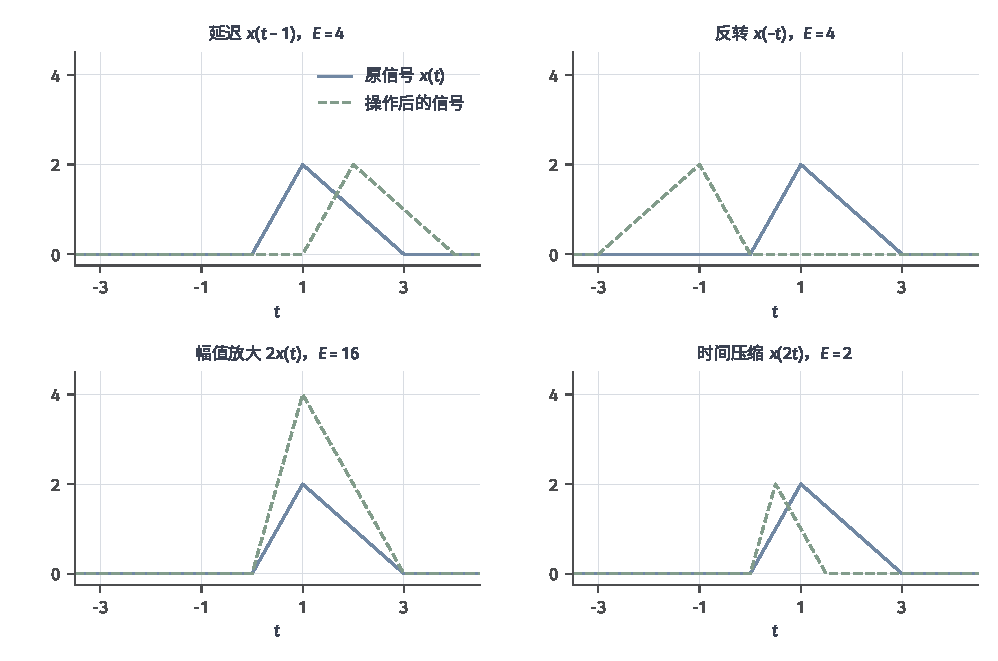
\includegraphics[width=169.0mm]{figures/01-mathematical-preliminaries-upper/07-signals/matplotlib/signal-basic-operations/figure.pdf}
  \caption{对同一非对称三角脉冲分别延迟、反转、放大幅值和压缩时间。
  每幅图的蓝线都是式~\eqref{eq:signal-asymmetric-wave}的原信号，绿线为指定操作结果，
  横轴为时间、纵轴为幅值，坐标尺度一致。平移和反转保持整轴能量$4$，幅值乘$2$使能量变为$16$，
  时间压缩一半使能量变为$2$；各图均在整轴零值背景下观察，不作窗口裁剪。}
  \label{fig:signal-basic-operations}
\end{figure*}

\subsection{信号之间的映射}
\label{sec:signal-input-output-maps}
\label{sec:signal-analysis-discrete-filtering}

一个系统是把输入信号映为输出信号的规则$y=\mathcal Hx$。
线性时不变系统之所以能用一条脉冲响应完全刻画，是因为线性让任意输入能拆成脉冲的加权和，
平移不变又让每个脉冲的响应只是同一条$h$的平移；对一般系统，
在有限位置上，线性规则可以写成$y[n]=\sum_r K[n,r]x[r]$，
其中$K[n,r]$说明位置$r$的单位输入怎样影响位置$n$的输出。
整轴表达还需要收敛条件，不能仅凭这个形式就交换无穷求和。
若输入、输出有$d_{\mathrm{in}}$和$d_{\mathrm{out}}$个通道，
则$K[n,r]$应为$d_{\mathrm{out}}\times d_{\mathrm{in}}$矩阵，
矩阵乘法负责混合通道、求和负责汇总时间位置，两者职责不同。

这里的因果性只表示“不读取未来输入”：若两条输入在所有$r\leq n$的位置相同，
它们在时刻$n$的输出必须相同。对可用脉冲逐项检验的线性核映射，
这等价于$r>n$时$K[n,r]=0$。
输入输出因果性约束的是读取时序；干预问题则比较变量机制被指定改变后的响应，
并需要明确干预时保持哪些其他机制不变，相关工具可参考
\BookChapterRef{chap:causal-inference}{卷2《数学准备：概率、因果与决策》的“因果响应”章}。
只按过去顺序计算一个预测量，不会自动证明其统计关系具有干预含义。

\subsubsection{线性时不变条件下的卷积映射}
\label{sec:signal-analysis-lti-convolution}

设系统已经给出原点处一个单位脉冲的响应。
这里先说明为什么值得对系统施加这两条限制。真实系统——固定的电路、参数不随时间改变的
平滑滤波器、权重恒定的卷积层——往往满足两条性质：相同波形晚一点出现，输出只整体平移而形状不变；
两路输入相加时，输出也相加。在这类系统下，系统行为完全由“原点一个单位输入的响应”决定，
从而可以把任意输入的计算化简为一次卷积；一般的时变或非线性系统则没有这种化简。
具体地说，如果其他位置的脉冲只使这条响应相应平移，而多个脉冲的响应又能按输入幅值相加，
我们就能由这一条响应算出全部有限输入的输出。前一个要求是平移不变，后一个要求是线性，
二者分别约束不同的行为。
\begin{definition}[线性时不变系统]
  \label{def:signal-analysis-lti-system}
  设输入、输出信号类为平移封闭的向量空间。若对任意标量$a,b$及输入$x,z$有
  $\mathcal H(ax+bz)=a\mathcal Hx+b\mathcal Hz$，称$\mathcal H$线性。
  若对每个允许的平移量$s$有
  \[
    \mathcal H(T_sx)=T_s(\mathcal Hx),
  \]
  称其具有\term{平移不变性}（shift invariance）。
  离散时间的平移量$s\in\mathbb Z$，连续时间的平移量$s\in\mathbb R$。
  同时满足两者的系统称为线性时不变系统（linear time-invariant system, LTI）。
\end{definition}
这里说的是输入整体移动后输出同样移动，并不是输出保持在原位置。
逐点平方$\mathcal Hx[n]=x[n]^2$平移不变却不线性，
位置加权$\mathcal Hx[n]=n\,x[n]$线性却不平移不变。
是否在每个位置调用了同一段程序，不足以替代这两项等式。

令$h=\mathcal H\delta$，称为\term{脉冲响应}（impulse response）。
有限支撑输入可按式~\eqref{eq:signal-analysis-impulse-expansion}作有限展开，
线性性与平移不变性给出
\begin{align}
  (\mathcal Hx)[n]
  &=\mathcal H\left(\sum_r x[r]T_r\delta\right)[n]\notag\\
  &=\sum_r x[r](T_rh)[n]=\sum_r x[r]h[n-r].
  \label{eq:signal-analysis-lti-convolution}
\end{align}
它把各个位置输入所触发的响应相加。
对$x\in\ell_1(\mathbb Z)$，还需要
$\mathcal H:\ell_1\to\ell_1$是有界线性且平移不变的算子，
即存在常数$C$使$\|\mathcal Hx\|_1\leq C\|x\|_1$。
令$x^{(K)}=\sum_{|r|\leq K}x[r]T_r\delta$，则$x^{(K)}\to x$于$\ell_1$，
有界性使$\mathcal Hx^{(K)}\to\mathcal Hx$。同时$h=\mathcal H\delta\in\ell_1$，且
\[
  \sum_n\sum_r|x[r]h[n-r]|=\|x\|_1\|h\|_1<\infty.
\]
因此卷积和绝对收敛，有限截断的卷积也在$\ell_1$中趋于该和，
从而式~\eqref{eq:signal-analysis-lti-convolution}能延伸到全部$\ell_1$输入。
这里不能省略连续性，直接把只对有限和成立的代数线性搬进无穷和。

这种求和称为\term{离散卷积}（discrete convolution），规则网格上也可用同一结构。
\begin{definition}[网格上的离散卷积]
  \label{def:signal-analysis-discrete-convolution}
  对$x,h\in\ell_1(\mathbb Z^d)$，定义
  \begin{equation}
    (x*h)[\bm n]=\sum_{\bm r\in\mathbb Z^d}x[\bm r]h[\bm n-\bm r].
    \label{eq:signal-analysis-discrete-multidimensional-convolution}
  \end{equation}
  这里$\bm n,\bm r$为网格位置，$h$称为\term{卷积核}（convolution kernel）。
  各位置的和绝对收敛，输出仍属于$\ell_1(\mathbb Z^d)$。
\end{definition}
存在性可直接检查：对非负项换序并令$\bm s=\bm n-\bm r$，有
\[
  \sum_{\bm n}\sum_{\bm r}|x[\bm r]h[\bm n-\bm r]|
  =\left(\sum_{\bm r}|x[\bm r]|\right)
   \left(\sum_{\bm s}|h[\bm s]|\right)<\infty.
\]
所以每个内层和都有限，并得到
$\|x*h\|_1\leq\|x\|_1\|h\|_1$。
核为有限支撑时，对任何逐点有限的输入也可作有限和，但输出不因此必属$\ell_1$。
一维记法为
\begin{equation}
  (x*h)[n]=\sum_{r\in\mathbb Z}x[r]h[n-r].
  \label{eq:signal-analysis-linear-convolution}
\end{equation}
固定$n$后，$r$增加时核索引$n-r$减小，这就是核的反向读取。
令$s=n-r$可得$(x*h)[n]=\sum_s h[s]x[n-s]=(h*x)[n]$，故有交换律；
在绝对可和等允许换序的条件下还给出结合律和分配律。
若对所有$r<0$都有$h[r]=0$，则$y[n]=\sum_r h[r]x[n-r]$只用当前及过去输入，
系统因果；一般LTI则不必因果，例如三点中心均值会用到$x[n+1]$。

离散卷积逐位置求和。连续时间没有可逐个枚举的位置，因此要用积分累计输入
与平移核的乘积，不能直接照搬离散的逐项求和。对下面的$L^1$函数，
积分只需在几乎处处的位置绝对收敛、并使所得函数整体可积，就能定义一个$L^1$元素；
若要读取某个指定位置的卷积值，还要单独检查该处收敛或补充更强条件。
\begin{definition}[连续卷积]
  \label{def:signal-analysis-continuous-convolution}
  设$f,g\in L^1(\mathbb R^d)$，定义
  \begin{equation}
    (f*g)(\bm t)=\int_{\mathbb R^d}f(\bm\tau)g(\bm t-\bm\tau)\,\mathrm d\bm\tau.
    \label{eq:signal-analysis-continuous-convolution}
  \end{equation}
  积分对几乎处处的$\bm t$绝对收敛，并定义$L^1(\mathbb R^d)$中的元素。
\end{definition}
由定理~\ref{thm:analysis-tonelli-fubini}，对非负函数换序并平移换元，
\[
  \int_{\mathbb R^d}\int_{\mathbb R^d}
  |f(\bm\tau)g(\bm t-\bm\tau)|\,\mathrm d\bm\tau\,\mathrm d\bm t
  =\|f\|_{L^1}\|g\|_{L^1}<\infty.
\]
内层积分因而几乎处处有限，且$\|f*g\|_{L^1}\leq\|f\|_{L^1}\|g\|_{L^1}$。
换元和换序同样给出交换律、结合律，但$L^1$假设不保证每个指定点的积分都有限。
这里定义的是两个普通可积函数的卷积，并非所有连续时间LTI算子都具有普通$L^1$核。
例如恒等映射是LTI，它的单位脉冲响应可用Dirac分布（Dirac distribution）
$\delta_0$描述。这里“分布”采用广义函数的用语：这个对象作用于光滑紧支撑的
测试函数$\phi$时返回$\delta_0(\phi)=\phi(0)$，也就是零点单位质量对$\phi$的积分。
对光滑紧支撑的$f$，卷积让它读取$\tau\mapsto f(t-\tau)$在零点的值，
于是$(f*\delta_0)(t)=f(t)$，正好实现恒等映射。
普通函数$\mathbb I_{\{0\}}$的Lebesgue积分却是零，不能承担这种单位质量，
所以不能把离散$\delta[k]$直接当作连续可积核。
这里不调用一般分布理论来证明所有连续系统的核表示。

\begin{example}[区间重叠产生三角形响应]
  \label{ex:signal-analysis-continuous-overlap}
  取$f(t)=g(t)=\mathbb I_{[0,1]}(t)$。两个因子同时为$1$要求
  $\tau\in[0,1]\cap[t-1,t]$，因此
  \[
    (f*g)(t)=
    \begin{cases}
      t,&0\leq t\leq1,\\
      2-t,&1<t\leq2,\\
      0,&\text{其余位置}.
    \end{cases}
  \]
  输出先随重叠长度增大而上升，再随重叠减小而下降。
  二维指示函数的相应积分计算重叠面积，一般带符号核则计算加权贡献，
  不能都解释为几何大小。
\end{example}
图~\ref{fig:reader-continuous-convolution-overlap}区分输出位置$t$和积分变量$\tau$。
三角形输出不是把两个输入图形相加，而是把每个$t$处的重叠长度汇成一条曲线。
\begin{figure*}[htbp]
  \centering
  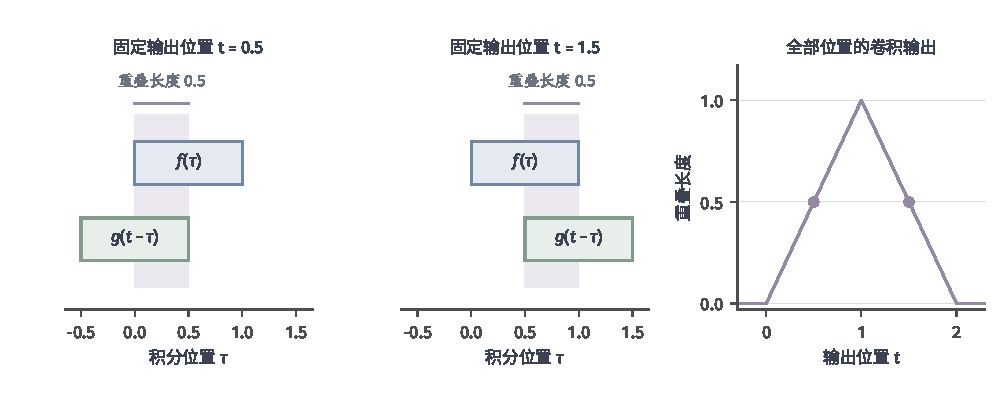
\includegraphics[width=169.0mm]{figures/01-mathematical-preliminaries-upper/07-signals/matplotlib/reader-continuous-convolution-overlap/figure.pdf}
  \caption{教学函数$f=g=\mathbb I_{[0,1]}$的连续卷积。左两图分别固定$t=0.5$与$t=1.5$，
  蓝色为$f(\tau)$的支撑，绿色为$g(t-\tau)$的支撑，紫色重叠区间的长度均为$0.5$。
  右图汇总全部$t$处的重叠长度，在$t=1$时达到$1$。
  左图横轴$\tau$用于积分，右图横轴$t$标记输出位置。}
  \label{fig:reader-continuous-convolution-overlap}
\end{figure*}

回到有限输入。若$x,h$的支撑分别为$0,\ldots,m-1$和$0,\ldots,r-1$，
零延拓线性卷积只可能在$0,\ldots,m+r-2$非零，完整输出长度为$m+r-1$。
贯穿例逐项为
\begin{align*}
  (x*h)[0]&=1,\\
  (x*h)[1]&=2-1=1,\\
  (x*h)[2]&=1-2=-1,\\
  (x*h)[3]&=-1.
\end{align*}
即
\begin{equation}
  \bm x*\bm h=(1,1,-1,-1).
  \label{eq:signal-analysis-running-linear-convolution}
\end{equation}
这个核计算当前值减去前一个值，首尾还包含零延拓带来的跳变。
特别是第一项之前补的是$0$，所以首项为$1-0=1$。
长度$N$的循环索引则在一个周期内求和：
这与前面“把数组首尾相接”的边界约定对应；也正因为首尾相接，
求和下标要用模$N$回绕，否则越界项无处安放。
\begin{equation}
  (x*_Nh)[n]=\sum_{r=0}^{N-1}x[r]h[(n-r)\bmod N],
  \qquad n=0,\ldots,N-1.
  \label{eq:signal-analysis-circular-convolution}
\end{equation}
\begin{definition}[循环卷积]
  \label{def:signal-analysis-circular-convolution}
  对长度$N$的实或复序列，式~\eqref{eq:signal-analysis-circular-convolution}
  定义其\term{循环卷积}（circular convolution），输出仍有$N$项。
  它在有限循环索引集上求和，不是两条周期延拓序列在整数轴上的无穷卷积。
\end{definition}
把$h$补成$(1,-1,0)$并取$N=3$，得到$x*_3h=(0,1,-1)$。
此时第一项的前一个值是记录末项$1$，所以首项变为$1-1=0$。
完整线性卷积的末项$-1$回绕到首项，与$1$相消；并不是直接删掉了末项。
若对两条周期序列在整轴无穷求和，同一贡献会被重复无穷次。
这里改变的是窗口外怎样连接。FFT只能加速已经选定的映射，不能决定首尾应该怎样连接；
若要用循环计算得到四项完整线性输出，必须补零到足以容纳这四项，避免回绕。
图~\ref{fig:signal-convolution-boundaries}对比零延拓与循环边界下的输出。
\begin{figure}[!htb]
  \centering
  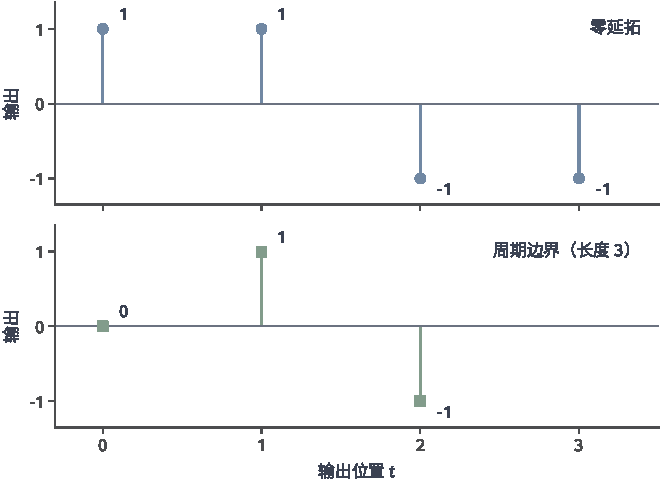
\includegraphics[width=112.0mm]{figures/01-mathematical-preliminaries-upper/07-signals/matplotlib/signal-convolution-boundaries/figure.pdf}
  \caption{输入$(1,2,1)$与核$(1,-1)$的边界比较。蓝色圆点采用零延拓，给出四项线性卷积；
  绿色方点采用长度$3$的循环边界，末项$-1$回到首项并与$1$抵消。
  竖线连接零基线与各离散输出，不定义整数之间的信号值。}
  \label{fig:signal-convolution-boundaries}
\end{figure}

固定输入输出位置后，线性卷积是Toeplitz矩阵乘法，循环卷积是循环矩阵乘法。
这两类特殊矩阵的出现不是巧合：卷积核在每个输出位置都按相同的相对次序使用、
只是整体平移，写成矩阵后同一核元素自然沿对角线重复，这正是线性时不变系统
“同一组权重在所有位置共享”的代数表现。
例如同一个贯穿例给出
\begin{gather*}
  \begin{bmatrix}
    1&0&0\\-1&1&0\\0&-1&1\\0&0&-1
  \end{bmatrix}
  \begin{bmatrix}1\\2\\1\end{bmatrix}
  =\begin{bmatrix}1\\1\\-1\\-1\end{bmatrix},\\
  \begin{bmatrix}1&0&-1\\-1&1&0\\0&-1&1\end{bmatrix}
  \begin{bmatrix}1\\2\\1\end{bmatrix}
  =\begin{bmatrix}0\\1\\-1\end{bmatrix}.
\end{gather*}
重复的对角线反映参数共享，边界则改变矩阵的首尾行。
无限网格或循环群上的平移不变性是精确的；有限区间采用零填充、反射或截取后，
通常不再具有同一意义下的全局平移不变性。

“valid”只保留核完全落在已知输入内、不需要补任何外部值的输出（卷积网络里常叫“有效填充”）。
按$h[0],\ldots,h[r-1]$的因果索引，当$m\geq r$时保留$n=r-1,\ldots,m-1$，
共$m-r+1$项；$m<r$时核比输入还长，没有这样的输出。
还要提醒，很多库里名为“same”的输出只是长度与输入相同，具体在左右各补多少、从哪里截取
并没有统一规定，不能只凭名称确定。表~\ref{tab:signal-boundary-conventions}把延拓和输出选择分开，
后文FFT也必须遵守同一约定。
\begin{table*}[!htb]
  \centering
  \begin{tabularx}{\linewidth}{lXXX}
    \toprule
    约定 & 区间外输入 & 保留输出 & 贯穿例\\
    \midrule
    完整线性卷积 & 零延拓 & $0,\ldots,m+r-2$ & $(1,1,-1,-1)$\\
    有效区间选段 & 不使用区间外值 & $r-1,\ldots,m-1$，$m\geq r$ & $(1,-1)$\\
    $N$点循环卷积 & 周期边界 & $0,\ldots,N-1$ & $N=3$时$(0,1,-1)$\\
    \bottomrule
  \end{tabularx}
  \caption{边界延拓与输出选段。$m$为输入长度，$r$为核长度，使用本章因果核索引。
  有效选段不是另一种卷积定义，循环边界也不是零边界的近似。}
  \label{tab:signal-boundary-conventions}
\end{table*}

有了有限DFT，循环卷积就能在频率坐标中逐项计算。
\begin{theorem}[离散循环卷积定理]
  \label{thm:signal-analysis-circular-convolution-theorem}
  设$x,h$为长度$N$的复序列，采用式~\eqref{eq:signal-analysis-dft}的约定，则
  \[
    \widehat{x*_Nh}[k]=\widehat x[k]\widehat h[k],\qquad k=0,\ldots,N-1.
  \]
\end{theorem}
\begin{proof}
  令$a=(n-r)\bmod N$，直接换有限求和的索引，
  \begin{align*}
    \widehat{x*_Nh}[k]
    &=\sum_{n=0}^{N-1}\sum_{r=0}^{N-1}
      x[r]h[(n-r)\bmod N]\omega_N^{kn}\\
    &=\sum_{r=0}^{N-1}\sum_{a=0}^{N-1}
      x[r]h[a]\omega_N^{k(r+a)}\\
    &=\left(\sum_{r=0}^{N-1}x[r]\omega_N^{kr}\right)
      \left(\sum_{a=0}^{N-1}h[a]\omega_N^{ka}\right).
  \end{align*}
  固定$r$后，$n$遍历一个周期使$a$也恰遍历一个周期。
  即使$n$与$r+a$相差$N$的整数倍，$\omega_N^{kN}=1$仍使指数相同。
  最后两项分别为$\widehat x[k]$与$\widehat h[k]$。
\end{proof}
于是
\begin{equation}
  x*_Nh=\mathcal F_N^{-1}\bigl(\mathcal F_N(x)\odot\mathcal F_N(h)\bigr).
  \label{eq:signal-analysis-frequency-domain-convolution}
\end{equation}
\BookEquationAliases{\label{eq:cnn-fft-convolution}
\label{eq:cnn-convolution-theorem-derivation}}
若$\bm C_h$为循环卷积矩阵，定理对所有$x$成立，故
$\bm F\bm C_h=\operatorname{diag}(\widehat{\bm h})\bm F$，从而
$\bm C_h=\bm F^{-1}\operatorname{diag}(\widehat{\bm h})\bm F$。
这完整说明DFT如何对角化循环卷积：核的DFT系数就是各频率模式的特征值。
要用它得到完整线性卷积，两个输入都必须补零到
\begin{equation}
  N\geq m+r-1.
  \label{eq:signal-analysis-linear-padding-condition}
\end{equation}
因为此时所有非零输出索引都小于$N$，不会回绕。
$N\geq\max(m,r)$只保证装下输入，不保证装下输出。

二维循环卷积按两个坐标分别取模，使用
式~\eqref{eq:signal-multidimensional-dft}，同样的有限换元给出
$\mathcal F(x*_{\mathrm{circ}}h)=X\odot H$。
输入支持为$W\times H_0$、核支持为$m\times r$且各从原点开始时，
线性输出支持至多为$(W+m-1)\times(H_0+r-1)$。
所以逐轴补零条件是$N_1\geq W+m-1$、$N_2\geq H_0+r-1$，
不是只让总像素数大于两个输入的总大小。
若$\bm F$为未归一化的网格DFT矩阵、$P=N_1N_2$，
则$\bm Q=\bm F/\sqrt P$酉，循环卷积矩阵满足
\begin{equation}
 \bm C_h=\bm Q^*\operatorname{diag}(\bm F\bm h)\bm Q.
 \label{eq:signal-multidimensional-circulant}
\end{equation}
因为每个网格复指数同时是各轴循环平移的特征向量，
核的加权平移之和就在同一组基下逐元素相乘。
对角元是未归一化的$\bm F\bm h$，不能误换成$\bm Q\bm h$而漏掉$\sqrt P$。

整轴上的频率响应改用DTFT。若$h\in\ell_1$或具有有限支撑，
即使复指数$x[n]=e^{\mathrm i\omega n}$自身不在$\ell_1$中，仍有绝对收敛的和
\[
  (x*h)[n]=\sum_r h[r]e^{\mathrm i\omega(n-r)}
  =e^{\mathrm i\omega n}\sum_r h[r]e^{-\mathrm i\omega r}.
\]
输出保持频率不变，只乘以
\begin{equation}
  H(e^{\mathrm i\omega})=\sum_r h[r]e^{-\mathrm i\omega r},
  \label{eq:signal-analysis-filter-frequency-response}
\end{equation}
即\term{频率响应}（frequency response）。它是分析滤波器最有用的一个量：给定任意频率的正弦输入，
稳态输出仍是同一频率，只是幅度乘上$|H|$、相位加上$\arg H$。于是想知道滤波器是增强还是压制某段频率，
只需看$|H|$在那段取多大。模长给出放大或衰减，相角给出相位变化；除非相位随频率呈线性形式，
不能把所有频率的相位变化都叫同一个时间延迟。
对$x,h\in\ell_1$，绝对可和允许换序，直接得到
$Y(e^{\mathrm i\omega})=X(e^{\mathrm i\omega})H(e^{\mathrm i\omega})$。
同理，连续$L^1$卷积的傅里叶变换为$F(\Omega)G(\Omega)$，
其积分换序由前面的绝对积分界保证。
多维$\ell_1(\mathbb Z^d)$与$L^1(\mathbb R^d)$仍使用相同换元：
绝对和或积分界使各轴换序合法，所以也分别得到$Y=XH$。
这里扩大的是位置维数，可积条件并没有因此消失。

贯穿核的响应为$H(e^{\mathrm i\omega})=1-e^{-\mathrm i\omega}$，
模长为$2|\sin(\omega/2)|$。在主频率区间$|\omega|\leq\pi$内，
模长随$|\omega|$从$0$到$\pi$增大：常量模式被消去（这正是“差分”该有的表现，平的地方差为零），
低频缓变只被轻微削弱，较高频的差异更突出。这一比较按模$2\pi$重复，不能沿整个实频率轴作单调解释；
有限输入首尾仍受延拓影响。

前面是单通道。彩色图像或多传感器记录有多个通道，每个输出通道都可以由全部输入通道
按各自的核加权汇合，于是标量核自然升级为矩阵核：
\begin{equation}
  y_a[n]=\sum_{b=1}^{d_{\mathrm{in}}}\sum_{r\in\mathbb Z}
  H_{a,b}[r]x_b[n-r],
  \qquad a=1,\ldots,d_{\mathrm{out}}.
  \label{eq:signal-multichannel-convolution}
\end{equation}
各$H_{a,b}\in\ell_1$、各$x_b\in\ell_1$时，有限通道求和与前述界保证存在性；
有限核则在每个位置作有限计算。当相同输入输出通道数且$\bm H[r]$总是对角矩阵时，
各通道分别滤波而不混合；非对角元素允许输入通道$b$影响输出通道$a$。
记$\bm X(e^{\mathrm i\omega})$与$\bm Y(e^{\mathrm i\omega})$为各通道DTFT组成的向量，
$\bm H(e^{\mathrm i\omega})$的第$(a,b)$项为核$H_{a,b}$的DTFT，则整轴频域关系为
$\bm Y(e^{\mathrm i\omega})=\bm H(e^{\mathrm i\omega})\bm X(e^{\mathrm i\omega})$。
每个频率上是矩阵乘向量，不是把所有通道分别做一次标量乘法。

无时间记忆的特例是核只在滞后$0$处非零，即$\bm H[0]=\bm B$、其余为零，
这时不做任何跨时刻汇总，只在同一时刻用矩阵$\bm B$混合各个通道
（卷积网络中$1\times1$卷积、或单纯的通道线性组合就是这种情形）。
取式~\eqref{eq:signal-multichannel-record}中的记录及
$\bm B=\begin{bmatrix}1&1\\1&-1\end{bmatrix}$，有
\[
  \bm Y=\bm X\bm B^\top
  =\begin{bmatrix}1&1\\3&1\\3&-1\end{bmatrix}.
\]
如图~\ref{fig:signal-channel-mixing}所示，输出第一通道为和、第二通道为差，
三个时间位置未变。总能量从$11$变为$22$，因为$\bm B^\top\bm B=2\bm I$；
用$\bm B/\sqrt2$才能保持能量。混合前若两路未按时间对齐，矩阵计算本身不会修正偏移。
\begin{figure*}[htbp]
  \centering
  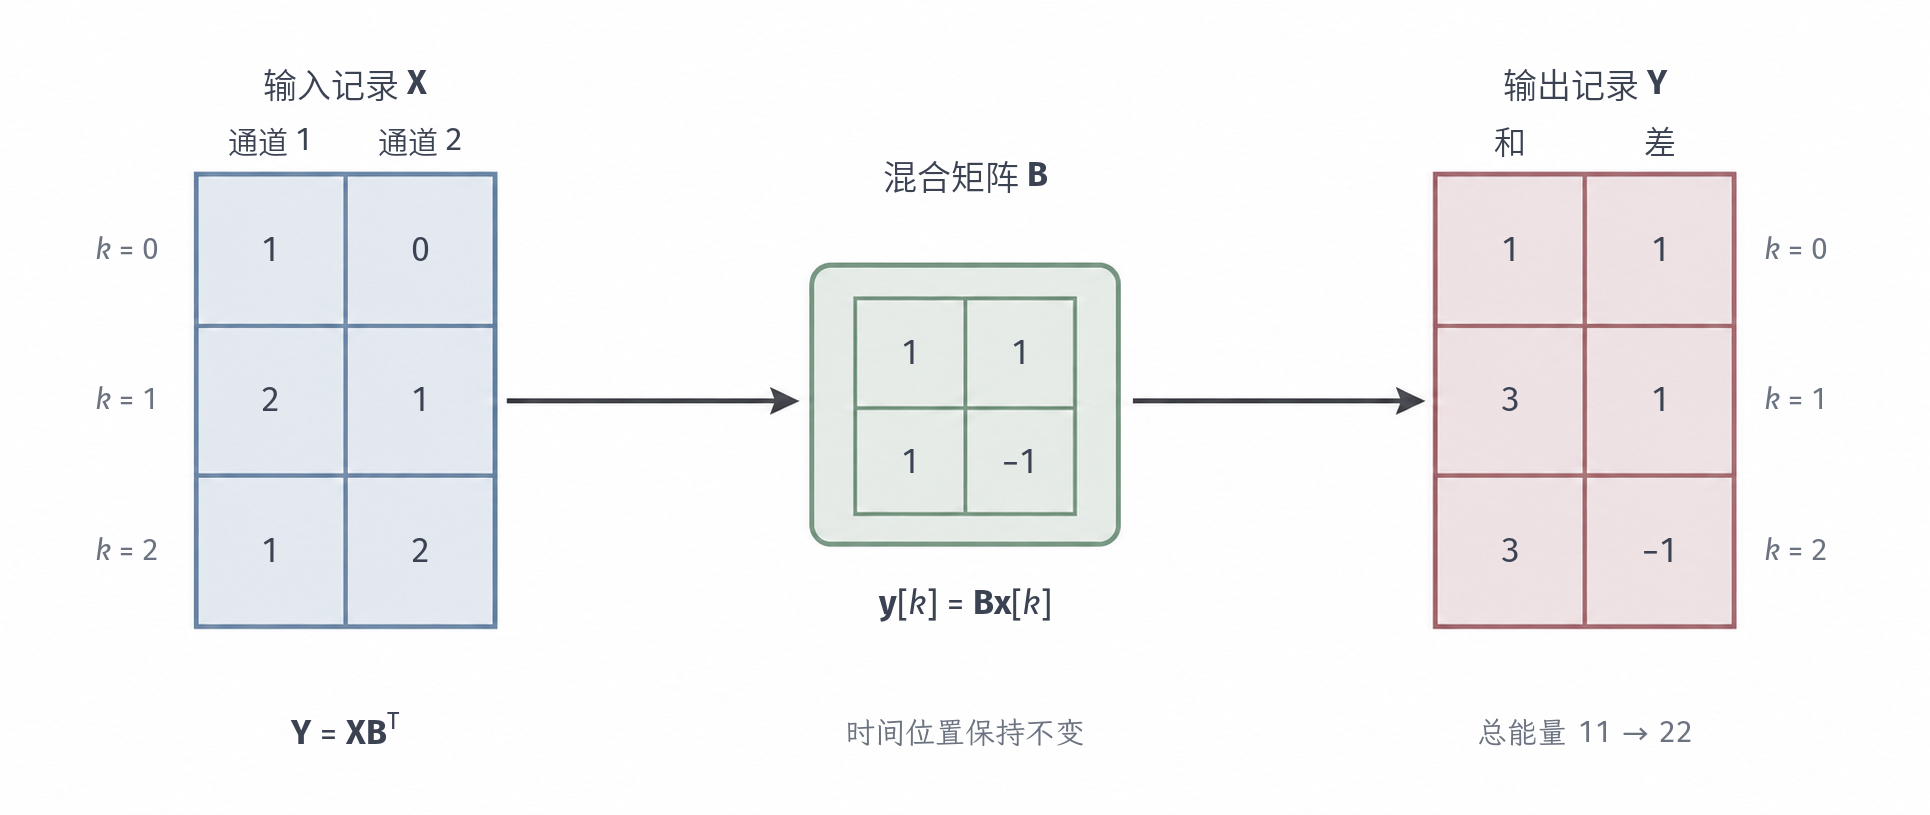
\includegraphics[width=168.998mm]{figures/01-mathematical-preliminaries-upper/07-signals/generated/signal-channel-mixing/figure.png}
  \caption{同一双通道三时刻记录的轴与混合。左侧行标记时间、列标记通道；
  中间矩阵$\bm B$对每一行对应的同时读数取和与差，右侧时间轴长度仍为$3$。
  通道混合不是时间平移，也不意味着两个输入通道独立；这里只使用当前时刻的值。}
  \label{fig:signal-channel-mixing}
\end{figure*}

\subsubsection{线性时变条件下的历史映射}

卷积要求核只依赖“隔了多久”而不依赖“现在几点”。但很多设备的增益会随时间变化：
比如录音设备电量逐渐下降，同样一个输入脉冲在早晨和晚上被放大的倍数可能不同。
这时系统仍然可以是线性的（两路声音一起输入，输出仍是各自输出之和），
却不再平移不变。一般地，用一个事先给定、随两个时刻变化的核表示
\begin{equation}
  \bm y[n]=\sum_{r\leq n}\bm K[n,r]\bm x[r].
  \label{eq:signal-given-time-varying-kernel}
\end{equation}
在有限历史窗口中它是有限和；在无限历史中则要另行保证收敛，
例如对有界输入可要求$\sum_{r\leq n}\|\bm K[n,r]\|<\infty$。
求和只取$r\leq n$规定了因果性，矩阵维度仍是
$d_{\mathrm{out}}\times d_{\mathrm{in}}$。
核事先固定、不随输入改变时，该表达满足叠加。
若还满足$\bm K[n+s,r+s]=\bm K[n,r]$，它才只依赖滞后$n-r$，
可以记成固定卷积核；不能只因它累加历史就省掉这项条件。

例如令$a[n]$在偶数时为$1$、奇数时为$2$，
$y[n]=a[n](x[n]+\tfrac12x[n-1])$。
它的两时刻核只在$r=n,n-1$非零，取值随绝对时刻$n$变化。
输入$\delta[n]$在时刻$0$给出$1$；把输入延迟一格后，时刻$1$的输出却是$2$，
而原输出延迟一格在该处仍为$1$，所以它不平移不变。
相反，事先给定$h[0]=0$、$h[r]=2^{-(r-1)}$（$r\geq1$）及负索引为零，
就定义了一个有衰减记忆的固定卷积核。对零延拓的$x=(1,2,1)$，
从时刻$0$起的前四项输出为$(0,1,5/2,9/4)$，每次都使用相同的滞后权重。

\paragraph{指数衰减的历史汇总}
一个常用的因果汇总是$y[n]=\alpha x[n]+(1-\alpha)y[n-1]$，
其中$0<\alpha\leq1$，初值$y[-1]$已经给定。逐次代入得到
\[
 y[n]=(1-\alpha)^{n+1}y[-1]
 +\alpha\sum_{r=0}^n(1-\alpha)^r x[n-r].
\]
自由项和输入项因而分开；零初值对应固定卷积核
$h[r]=\alpha(1-\alpha)^r$（$r\geq0$），其绝对和为$1$。
频率响应是几何级数
$H(e^{\mathrm i\omega})=\alpha/(1-(1-\alpha)e^{-\mathrm i\omega})$，
恒定输入的零频增益为$1$。初值和输入都在同一区间时，递推是凸组合，输出不会越出该区间。
从零初值接收单位阶跃时，输出为$1-(1-\alpha)^{n+1}$：
较小的$\alpha$给过去读数更长的记忆，也使阶跃响应更慢。
这是确定性的\term{指数平滑}（exponential smoothing），
不需要把读数先解释成随机噪声；非零初值下的整段映射仍含自由项。

这些例子都通过给定核来计算输入输出。内部状态演化也能产生固定核或两时刻核，
但构造时需要区分初始状态的自由响应、当前输入的直接项和输入驱动项。
状态演化中的有序矩阵乘积解释了核从何而来，本节先检验给定核所定义的映射。
若另加一个与输入无关且非零的自由响应，总映射一般是仿射而非线性，
不能仅因输入驱动部分线性就忽略这一差别。

\subsubsection{非线性条件下的输入输出映射}

前面的核都事先固定，不随输入变化。还有一类常见系统，权重本身由当前输入决定
（神经网络里的门控、激活都属于这种）。这时输出仍可写成某种加权形式，
但检验线性时必须把“权重随输入改变”也一起算进去，不能只看加权那一步。
一个最简单的非线性例子是逐点平方$(\mathcal Hx)[n]=x[n]^2$：输入取$1$时输出为$1$，
把输入加倍成$2$后输出变成$4$而不是$2$，所以不满足线性；
但它仍平移不变（输出只取决于同一位置），且只使用当前值，满足这里的因果性。

这个区分很有现实意义：它说明“逐点”“平移不变”并不等于“线性”，
卷积网络里夹在卷积之间的非线性激活虽然在每个位置用同一条规则，却破坏了叠加。

再看输入依赖门控
\[
  y[n]=g(x[n])x[n],\qquad g(v)=\frac1{1+e^{-v}}
\]
（此例取实数输入）。门控是由当前输入决定的权重。
记标量响应为$\varphi(v)=g(v)v$。输入$1$与$2$得到的比例分别是$g(1)$与$g(2)$，两者不同，
所以$\varphi(2)\neq2\varphi(1)$；在同一时刻把输入加倍，输出没有按相同比例变化。
尽管每个位置使用同一规则，叠加仍不成立。
更一般的$\sum_{r\leq n}K_x[n,r]x[r]$既要检查核如何依赖输入，
也要检查计算$K_x$时是否依赖未来输入值。求和表面上只到$n$，
不代表输入依赖的权重一定因果。

可微映射在固定输入附近可以线性化。先在每个位置考察平方这一标量映射，它满足
$(x_0+\varepsilon v)^2=x_0^2+2\varepsilon x_0v+\varepsilon^2v^2$，
一阶响应是$v\mapsto2x_0v$。它依赖展开位置$x_0$，只描述小扰动；
不能据此给全部输入配同一个频率响应。
状态参数若由输入选择，也要连同它们对输入的响应一起检验叠加，
不能把固定输入附近的线性化当作全局固定核。

\subsection{信号的相关运算}
\label{sec:signal-template-correlation}

卷积叠加的是输入所激起的响应；另一个常见任务是“在一长段记录里找出某个已知波形出现在哪”，
比如在录音里定位一声特定的音、在图像里滑动一个小模板找相似图案。这时没有“系统响应”可言，
更自然的做法是让模板与记录中每个同样长度的片段逐点对齐、求内积：内积越大，该片段与模板越像。
卷积和这个操作（称为相关）在求和式上只差一个“核要不要反转”，但含义不同，必须分清。
采用本章方向约定，\term{互相关}（cross-correlation）为
\begin{equation}
  (x\star h)[n]=\sum_{r\in\mathbb Z}x[n+r]\overline{h[r]}.
  \label{eq:signal-analysis-cross-correlation}
\end{equation}
固定$n$后，比较的是片段$r\mapsto x[n+r]$与原方向模板$r\mapsto h[r]$；
若把该片段记为$x_n[r]=x[n+r]$，这个读数就是$\langle h,x_n\rangle$：
模板放在内积第一变量，因而对模板取共轭，对信号片段保持线性。
若$x,h\in\ell_2$，Cauchy--Schwarz保证每个$n$处绝对收敛；
有限模板则只需对应片段逐点有定义。

令$\widetilde h[r]=\overline{h[-r]}$，换元可得
\[
  (x*\widetilde h)[n]=\sum_s x[s]\overline{h[s-n]}
  =\sum_r x[n+r]\overline{h[r]}=(x\star h)[n].
\]
所以相关可以用共轭反转核的卷积实现，但模板自身仍按原方向比较。
多通道模板在同一$n$处按$\langle\bm h,\bm x_n\rangle$的顺序汇总：
$\sum_r\sum_c x_c[n+r]\overline{h_c[r]}$，
带权版本为$\sum_r\bm h[r]^*\bm W\bm x[n+r]$。
若作归一化，应同时使用当前片段与模板的非零范数；窗口或权重变化也会改变相似性。

仍取零延拓$x=(1,2,1)$、$h=(1,-1)$。
模板完全在输入内时，相关在$n=0,1$得到$1-2=-1$与$2-1=1$；
完整相关在$n=-1,0,1,2$依次为$(-1,-1,1,1)$。
完整卷积则在$n=0,1,2,3$得到$(1,1,-1,-1)$，
而valid卷积在$n=1,2$给出$(1,-1)$。
差异既来自核方向，也来自输出索引，不能只看数组长度就判断二者相同。
许多神经网络库把不反转实核的相关称为“卷积”，训练参数可以适应该约定；
但手算、复用核或推导伴随算子时，仍须明确反转、共轭、延拓及输出范围。

\paragraph{循环相关的频域计算}
若两条长度$N$的序列按周期延拓，
令$g[n]=\sum_{r=0}^{N-1}x[(n+r)\bmod N]\overline{h[r]}$。
在$g$的DFT中令$a=(n+r)\bmod N$，便有
\[
 G[k]=\sum_a x[a]e^{-2\pi\mathrm i ka/N}
       \sum_r\overline{h[r]}e^{2\pi\mathrm i kr/N}
     =X[k]\overline{H[k]} .
\]
这就是本章方向约定下的\term{相关定理}（correlation theorem）。
相应地$g=\operatorname{IDFT}(X\odot\overline H)$，
共轭在模板一侧。把相关次序颠倒会使相应的共轭与位移方向改变。
二维情形在每个坐标重复同一换元；
零延拓线性相关则要先补足支持，再把负位移输出重新编号。
例如$x=h=(1,0)$时循环相关为$(1,0)$，
DFT模平方为$(1,1)$，逆变换确实恢复它。
本段只用有限循环和，不把一般$\ell_2$相关的存在性
误当成其普通DTFT级数逐点收敛的保证。

图~\ref{fig:vol1-add-signal-correlation-direction}换用非对称实模板$(1,2)$，
把同一片段中的两个读数固定下来，只改变模板方向。
相关使用原方向模板，卷积在对应位置使用反向权重，因此两次点积可以给出不同结果。
\begin{figure}[!htb]
  \centering
  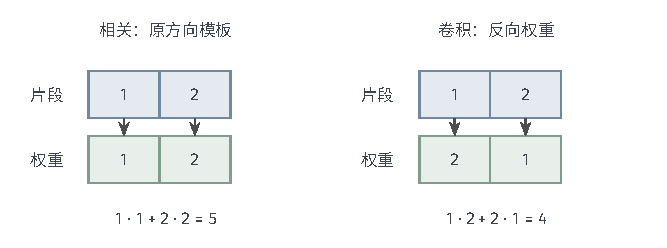
\includegraphics[width=112mm]{figures/01-mathematical-preliminaries-upper/00-shared/tikz/graphs-and-signals-comprehension-additions/signal-correlation-direction.pdf}
  \caption{零延拓信号$x=(1,2,1)$与额外教学模板$h=(1,2)$。
  两侧都只读取$x[0],x[1]$：左侧相关在$n=0$使用$h[0],h[1]$，得到$(x\star h)[0]=5$；
  右侧卷积在$n=1$使用$h[1],h[0]$，得到$(x*h)[1]=4$。
  蓝格为信号读数，绿格为参与同一位置乘法的权重。这里固定片段来比较方向，两个输出索引并不相同。}
  \label{fig:vol1-add-signal-correlation-direction}
\end{figure}

\subsection{网格变化的差分计算}
\label{sec:signal-grid-differences}

卷积既能平均邻域、把抖动抹平，也能反过来比较邻域之间的差，从而估计连续曲线的斜率或弯曲程度。
图像里找边缘用的就是后者：边缘两侧亮度相差大，局部差分值也大。
但离散读数终究只是网格上的几个点，用它们代替导数会带来误差，
网格越密越准，却又会把噪声的快速抖动一并放大。
下面先用Taylor展开说清每种差分近似的是什么、误差多大，
再用频率响应解释它保留和丢弃了什么，最后把“先平滑、再差分”组合成实用的边缘算子。

\subsubsection{一阶变化与二阶变化的近似}
令$x[\bm n]=f(h\bm n)$，$h>0$为各轴相同的网格步长，
$\bm e_j$为第$j$个坐标方向。定义
\begin{equation}
 \begin{aligned}
 D_j^+x[\bm n]&=\frac{x[\bm n+\bm e_j]-x[\bm n]}h,\\
 D_j^cx[\bm n]&=\frac{x[\bm n+\bm e_j]-x[\bm n-\bm e_j]}{2h},\\
 \Delta_hx[\bm n]&=\frac1{h^2}\sum_{j=1}^d
 \bigl(x[\bm n+\bm e_j]-2x[\bm n]+x[\bm n-\bm e_j]\bigr).
 \end{aligned}
 \label{eq:signal-grid-differences}
\end{equation}
在所考察点的邻域内，$f$有有界二阶导数时，前向差分与$\partial_jf$相差$O(h)$；
有有界三阶导数时，中心差分的两侧二阶项抵消，误差为$O(h^2)$。
有有界四阶导数时，对称相加再减$2f$给出
$\Delta_hx=\Delta f+O(h^2)$。这些界来自第~\ref{chap:univariate-differentiation}章的Taylor展开，
要求邻域内的光滑性，不能直接解释跨跳跃处的“真实导数”。
二维$\Delta_h$的五点核为
$h^{-2}\begin{bmatrix}0&1&0\\1&-4&1\\0&1&0\end{bmatrix}$。
常量给出零；对$f(t_1,t_2)=t_1^2+t_2^2$，每个内点给出$4$，
这也核对了步长的平方与符号。

采用整轴离散变换或循环边界时，三种乘子分别为
$(e^{\mathrm i\omega_j}-1)/h$、
$\mathrm i\sin\omega_j/h$和
$-4h^{-2}\sum_j\sin^2(\omega_j/2)$。
这三个乘子也解释了为什么“差分既能找边缘、又会放大噪声”：低频处（$\omega$接近$0$）
乘子很小，平缓背景被抑制；频率越高乘子越大，边缘对应的高频被增强，但噪声那种逐点乱跳
恰好在最高频，于是也被一起放大。还要注意一个盲点：中心差分在Nyquist频率（相邻点正负交替）
处乘子为零，所以并非所有“快速交替”都能被它发现——棋盘格那样$+1,-1,+1,-1$的模式
会被中心差分当成常量而漏掉。
$-\Delta_h$的乘子非负，与一般图上正半定Laplacian的常用符号相合；
连续$\Delta$及此处$\Delta_h$自身的频率乘子则非正。
有限数组的边界仍按先前延拓计算，不能把内部误差阶直接沿用到任意补边处。

\subsubsection{平滑与差分的组合}
直接用中心差分，噪声也会被当成边缘。一个直接的改进是先把邻域平均一下、再求差，
让参与差分的每个读数都先由几个点平均得到，噪声互相抵消而真正的边缘仍在。
令$s[-1],s[0],s[1]=(1,2,1)/4$，
先沿第二轴用$s$平滑，再沿第一轴作$D_1^c$，就是图像里常用的归一化Sobel型边缘算子。
其权重是两个一维核的外积；若以“原方向读模板”的相关形式列出，
第一轴差分权重为$(-1,0,1)/(2h)$。
改用本章的卷积形式须反转该奇核，符号随之改变。
例如$x[n_1,n_2]=2hn_1+3hn_2$在内部给出两方向读数$2$、$3$，
梯度模长为$\sqrt{13}$。用这种斜坡检验实现，比只看对称边缘更容易发现方向颠倒。
外积核的计算节省由后文核分离推导，不在这里另作一套算法。

若各个方向都先平滑，可使用归一化高斯核
\[
 G_\sigma(\bm t)=(2\pi\sigma^2)^{-d/2}
 e^{-\|\bm t\|^2/(2\sigma^2)}.
\]
直接求导给出
\[
 \Delta G_\sigma=
 \left(\frac{\|\bm t\|^2}{\sigma^4}-\frac d{\sigma^2}\right)G_\sigma,
 \qquad \partial_\sigma G_\sigma=\sigma\Delta G_\sigma .
\]
对有界输入或绝对可积输入，高斯导数的衰减允许把空间微分放入卷积。
因此$\Delta(G_\sigma*f)=(\Delta G_\sigma)*f$：
\term{高斯拉普拉斯}（Laplacian of Gaussian, LoG）先压制细尺度变化，再读二阶变化。
对固定$\sigma>0$且$k$接近$1$，按尺度变量Taylor展开又有
$G_{k\sigma}-G_\sigma=(k-1)\sigma^2\Delta G_\sigma+
O((k-1)^2)$，余项在固定紧集上一致。
这解释\term{高斯差分}（difference of Gaussians, DoG）为何能近似尺度归一化的LoG；
相差很大的两个尺度不能忽略该余项。连续恒等式与截断、离散化后的核仍须分别检验。

“平滑”和“差分”在真实画面上的对比非常直接，图~\ref{fig:real-image-filter}三幅图给出同一张照片：
中间用$5\times5$均值核滤波后，树叶和纹理被抹平、边缘也变软（高频被压制）；
右侧用Sobel算局部差后，平缓的天空和墙面变成黑色，只有屋檐、门窗、树冠轮廓发亮。
这说明卷积核实际上是在挑选频率——想去掉抖动就用低通平滑，想找边缘就让高频通过。
\begin{figure*}[htbp]
  \centering
  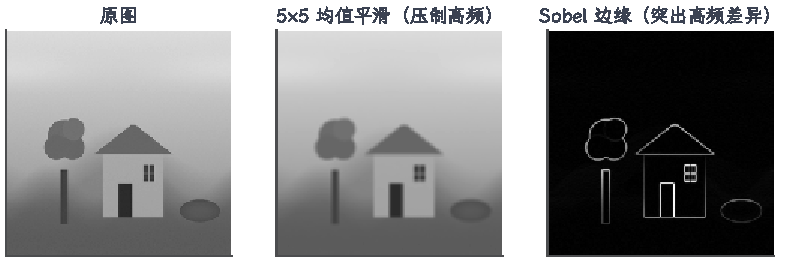
\includegraphics[width=0.96\textwidth]{figures/01-mathematical-preliminaries-upper/07-signals/matplotlib/teaching-signals-real-image/real-image-filter.pdf}
  \caption{同一灰度照片上的两个卷积。中：$5\times5$均值平滑（低通），细纹理被压制、边缘变软；
  右：Sobel边缘算子（突出高频差异），平缓区域变黑、各物体轮廓发亮。
  两个核都只做局部加权和，差别只在权重如何随位置变化。教学画面由脚本确定性生成。}
  \label{fig:real-image-filter}
\end{figure*}

\subsection{分辨率改变下的多尺度映射}
\label{sec:signal-multiscale-maps}

把一张图缩小一半，直觉上只要每隔一个像素取一个就行；但这样直接抽取会丢掉一半位置，
一旦原图带有细密条纹，抽出来的图可能把“密条纹”错看成另一种“疏条纹”（混叠），
而且仅凭缩小后的图无法还原。
即使画面里没有规则条纹，直接隔点抽取也会让斜线和圆弧出现明显的“台阶”：
图~\ref{fig:real-image-downsampling}把照片缩到$1/4$，直接抽取后屋顶斜边呈锯齿状、
门窗格子也错了位；先对$4\times4$小块取平均再抽取，则在缩小前先把亚像素的变化压掉，
边缘虽然变软，却没有那些突兀的台阶——这就是后面“先抗混叠滤波、再抽取”的直观来源。
要想缩小之后还能无损恢复，就得在缩小的同时，
把那些被丢掉的细微变化另存一份。我们先用最简单的“两两取平均、两两取差”构造一个
完全可逆的最小例子，看清平均和细节各自保存了什么；抽取引入的频率重叠称为
\term{混叠}（aliasing），再研究一般的两通道滤波如何消去这种重叠；
最后用“粗层预测加残差”解释图像金字塔的重建。这里的可逆性都指保留了全部系数，
绝不意味着只留一张低分辨率图就能恢复任意输入。
\begin{figure*}[htbp]
  \centering
  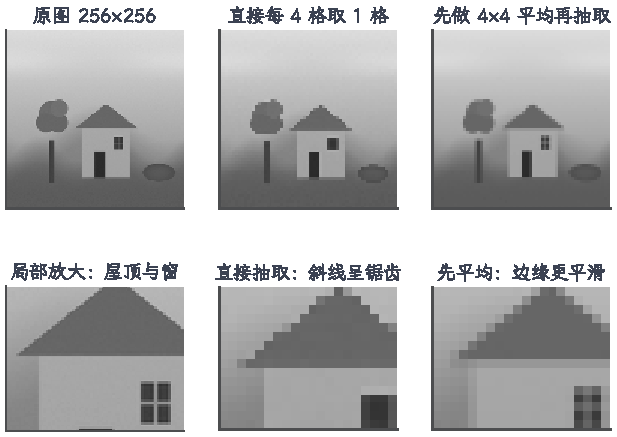
\includegraphics[width=0.95\textwidth]{figures/01-mathematical-preliminaries-upper/07-signals/matplotlib/teaching-signals-real-image/real-image-downsampling.pdf}
  \caption{把照片缩到$1/4$的两种做法。上排为整图、下排为屋顶与窗的局部放大：
  直接每$4$格取$1$格会让屋顶斜边呈阶梯状、门窗格子错位（混叠/锯齿）；
  先对$4\times4$小块取平均再抽取，边缘更平滑，因为高频在抽取前已被压低。
  教学画面由脚本确定性生成。}
  \label{fig:real-image-downsampling}
\end{figure*}

\subsubsection{局部平均与细节的正交分解}
\label{sec:signal-haar-decomposition}
先看最小的可逆缩小：把相邻两个读数$(x[2k],x[2k+1])$看成一组，用一个数记它们的“平均水平”$a[k]$，
用另一个数记它们的“差别”$d[k]$。两个数的信息恰好等于原来两个读数，所以可以无损拆开、
也能无损拼回（下面的$1/\sqrt2$只是为了让能量保持不变）。对偶数长度$2M$的记录，逐对定义
\begin{equation}
 a[k]=\frac{x[2k]+x[2k+1]}{\sqrt2},\qquad
 d[k]=\frac{x[2k]-x[2k+1]}{\sqrt2}.
 \label{eq:signal-haar-pair}
\end{equation}
逆式为$x[2k]=(a[k]+d[k])/\sqrt2$、
$x[2k+1]=(a[k]-d[k])/\sqrt2$。
两行权重正交且长度为一，故每对满足
$|x[2k]|^2+|x[2k+1]|^2=|a[k]|^2+|d[k]|^2$，即拆成平均和差别后总能量不变。
这就是有限记录上的\term{Haar变换}（Haar transform）。
例如$(2,4,6,8)$变为$a=(3\sqrt2,7\sqrt2)$、
$d=(-\sqrt2,-\sqrt2)$，总能量仍是$120$。
若舍去全部细节，逆式把每一对替换成该对平均，
误差平方就是$|d[0]|^2+|d[1]|^2=4$。

长度为$2^J$时，可对平均分量重复同一分解。
在原记录空间中，令$V_j$为在每个长度$2^j$的对齐块内恒定的数组，
则$V_0\supset V_1\supset\cdots\supset V_J$。
每对相邻粗块的相反符号读数张成细节空间$W_j$，有
$V_{j-1}=V_j\oplus W_j$，直和按离散内积正交。
逐层平均是投影到更小的空间，细节记录两级之间的正交差。
这是有限维的\term{多分辨率分析}（multiresolution analysis）；
不在这里把有限数组直接等同于整轴函数空间的完备小波系。

二维时沿两轴分别作同一变换，得到平均--平均、差--平均、平均--差、差--差四个子带。
对子块$\begin{bmatrix}1&2\\3&4\end{bmatrix}$，
相应读数为$5,-2,-1,0$，平方和为$30$。
差作用在哪个轴，就对哪个轴的变化敏感；边缘延伸方向与变化法向须分清。

\subsubsection{双通道滤波下的完全重建}
\label{sec:signal-perfect-reconstruction}
Haar里“平均”和“差别”都只用相邻两点，能处理的变化很有限。自然的推广是用两个较长的滤波器：
一个低通看整体趋势、一个高通看细节，各自抽取一半，再在重建端把两路合起来。
这里要扭转一个直觉：缩小后的每一路单独都不可逆（平均丢了差别，高通也丢了趋势），
关键在于两路合起来要把信息凑齐——重建端要让低通分支造成的混叠恰好被高通分支抵消。
下面推导这种“抵消”在什么条件下发生。
设有限分析核$h_0,h_1$先卷积再保留偶数项，得到
$a_j[k]=(h_j*x)[2k]$；合成时在奇数位置插零，再分别用有限核$g_j$卷积相加。
本段在整轴有限支撑输入上推导，故所有变换与换序都是有限运算。
记$H_j(z)=\sum_nh_j[n]z^{-n}$、$G_j(z)=\sum_ng_j[n]z^{-n}$。
这里用$z^{-1}$表示一个单位延迟，与前面只记录数组位置的正幂多项式区别开来。
取偶数项再插零，会把某序列的变换$U(z)$改成
$(U(z)+U(-z))/2$。因为两项相加恰好消去所有奇数幂，合成输出满足
\begin{equation}
 \begin{aligned}
 \widehat X(z)&=\frac12\sum_{j=0}^1G_j(z)H_j(z)X(z)\\
 &\quad+\frac12\sum_{j=0}^1G_j(z)H_j(-z)X(-z).
 \end{aligned}
 \label{eq:signal-two-channel-transfer}
\end{equation}
第二项含有$X(-z)$，正是抽取时折回来的那个“混叠副本”。要让输出只含原信号、不含混叠，
就要让两路在这一项上恰好抵消；同时让第一项整体等于一个纯延迟$2z^{-\ell}$
（允许重建结果比输入晚$\ell$格，波形不变）。这两个要求写成
\begin{equation}
 \sum_jG_j(z)H_j(-z)=0,\qquad
 \sum_jG_j(z)H_j(z)=2z^{-\ell}.
 \label{eq:signal-perfect-reconstruction-conditions}
\end{equation}
第一式让两个分支折回来的副本相加为零（混叠抵消），第二式保证原信号整体无失真地通过
（只差一个已知延迟）。充分性把条件代回重建式即可；必要性则分别取只在位置$0$为一、
和只在位置$1$为一的两个脉冲输入，前者使$X(z)=X(-z)=1$、后者使$X(-z)=-X(z)$，
比较两者的重建恒等式再相加、相减，就能分别定出两项系数。
这组条件说明：只把低通分支调得很平滑并不能保证无损，\term{完全重建}
（perfect reconstruction）要求的是两个分支在混叠项上精确配合。

例如取$H_0=(1+z^{-1})/\sqrt2$、
$H_1=(1-z^{-1})/\sqrt2$，
$G_0=(1+z^{-1})/\sqrt2$、
$G_1=(-1+z^{-1})/\sqrt2$。
第一组和为零，第二组和为$2z^{-1}$，所以重建结果是$x[n-1]$。
这里分析核把$x[2k]$与$x[2k-1]$配对，与式~\eqref{eq:signal-haar-pair}的分块原点不同，
补偿已知延迟后是同一种平均与差分解。
有限数组还必须选定兼容的延拓与抽取相位；任意裁去边缘会破坏上述整轴恒等式。

\subsubsection{粗细层之间的递归重建}
\label{sec:signal-pyramid-reconstruction}
Haar分解要求平均和细节正好正交，限制较强。实际的图像金字塔更朴素：先把图缩小存一份，
再记录“原图减去缩小后放大回来的预测”还差多少。这里的缩小和放大可以用任意约定的滤波器，
不必构成正交投影。设$D$是“低通后每轴抽取二倍”的固定缩小算子，
$U$是约定的插零加插值放大算子。令
\begin{equation}
 G_{j+1}=DG_j,\qquad L_j=G_j-UG_{j+1}.
 \label{eq:signal-laplacian-pyramid}
\end{equation}
粗层$G_{j+1}$给出低分辨率描述，残差$L_j$就是把粗层放大回原尺寸后仍对不上的那部分，
也就是用粗层预测原层时漏掉的细节。
保留最粗层$G_J$及全部$L_j$后，用$G_j=L_j+UG_{j+1}$从粗到细逐层恢复：
先把上一层放大，再加上当时存下的残差。
这由定义逐层恒等成立，不要求放大正好是缩小的逆（$UD=\bm I$）；
但同样不能据此宣称只留一张最粗的缩略图就能无损重建——残差一份都不能少。
当平滑采用高斯核或其离散近似时，粗层组成高斯金字塔，相应残差层组成拉普拉斯金字塔。
实际低通核不必是无限高斯；有限核、边界和$U$必须在分析与合成时一致。

二维每层像素数约减为四分之一，忽略取整边界后，
所有粗层的总像素数小于原图的$4/3$倍。金字塔残差仍按各自层的尺寸存放，
不能把这一计数误当作任意编码后的压缩率。
若每轴插值核的离散和为$2$，二维可分离插值核的和为$4$；
这一尺度用来补偿插零后常量平均的下降。保常量还要求各相位的核权重和都为$1$，
只检查总和并不足够。例如一维线性插值核
$(1/2,1,1/2)$的偶、奇两组权重和都为$1$，因此能恢复插零前的常量序列。

\subsection{离散幅度下的信号表示}
\label{sec:signal-quantized-representation}

前面所有表示都默认数值是精确的：DFT系数写多少就是多少，逆变换能一字不差地还原。
但计算机存储每个数只用有限个比特，灰度图像的像素通常也只取$0$到$255$的整数，
于是连续取值必须先“就近归到最近的若干档”之一，这一步叫量化。
量化和坐标变换是两件不同的事：DFT本身可逆，并不代表把系数四舍五入后还能精确还原。
本小节以实数读数及实正交变换为对象，先给出一个不依赖任何概率假设的确定性幅度误差界，
再说明预测编码为什么必须让发送端和接收端使用同一份“已经重建出来的历史”。
把误差当成随机噪声、讨论平均码长则属于另一类问题，这里只研究单条确定记录。

\subsubsection{均匀量化的幅度误差}
最常用的量化是均匀量化：先选定一个固定步长$\Delta$（相邻两档之差），再把每个值
就近归到$\Delta$的整数倍，即
$Q_\Delta(t)=\Delta\operatorname{round}(t/\Delta)$，中点（如恰好落在两档正中）
采用任一固定规则。这样每个值最多偏离真实值半个步长：
若量化格无限，或输入不超过有限量化器的可表示范围，就有
$|Q_\Delta(t)-t|\leq\Delta/2$。
若输入超出有限量化器的最大可表示值，会被强行截断（饱和），此时不再受这个界保证。
对$n$个读数，逐点误差平方至多$n\Delta^2/4$；
若正交变换的第$i$个系数采用步长$\Delta_i$，
则原空间的重建误差满足
\begin{equation}
 \|\widehat{\bm x}-\bm x\|_2^2
 =\sum_i|\widehat c_i-c_i|^2
 \leq\frac14\sum_i\Delta_i^2 .
 \label{eq:signal-quantization-bound}
\end{equation}
等号来自正交性，最后一步来自每个量化格的半宽。
例如两个系数步长分别为$1$、$2$时，误差范数至多$\sqrt5/2$。
这里没有假设误差均匀分布、互相独立或均值为零，
不能把$\Delta^2/12$当作所有输入共有的误差。
图像量化的效果一眼可见：图~\ref{fig:real-image-quantize}把每个像素的连续灰度就近归到
仅$4$个灰阶，天空和山坡的平滑渐变变成一圈圈分明的色带（等高线），细节也随之丢失；
这与坐标变换无关，纯粹是“用有限档表示连续值”付出的代价。
\begin{figure*}[htbp]
  \centering
  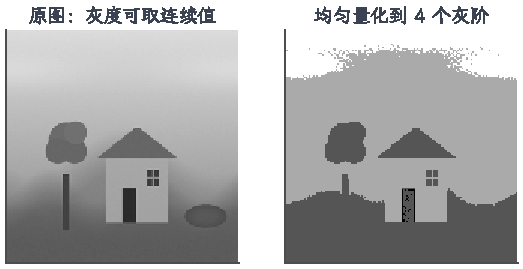
\includegraphics[width=0.78\textwidth]{figures/01-mathematical-preliminaries-upper/07-signals/matplotlib/teaching-signals-real-image/real-image-quantize.pdf}
  \caption{量化前后。左：每个像素可取连续灰度；右：均匀量化到仅$4$个灰阶后，
  天空与山坡的平滑渐变变成一圈圈分明的色带。量化是独立于DFT/DCT的又一步信息损失。
  教学画面由脚本确定性生成。}
  \label{fig:real-image-quantize}
\end{figure*}

\subsubsection{闭环预测下的差值编码}
许多信号相邻读数很接近（语音、温度都如此），与其存每个绝对值，不如只存“当前值比预测值
多了多少”：差值通常很小，用更少的档就能表示。但这里有个容易被忽略的一致性要求——
编码端作预测时，必须使用解码端将来真正能拿到的“已重建历史”，而不能用自己手上的原始值，
否则两边预测的基准不同，误差会逐格累积。令预测器按已经重建的历史产生$p[n]$，编码端量化
$r[n]=x[n]-p[n]$，发送$\widehat r[n]=r[n]+e[n]$。
解码端采用相同初始历史、同一预测规则和收到的量化差值，重建
$\widehat x[n]=p[n]+\widehat r[n]$。
按时间归纳，两端始终持有相同的重建历史，故预测$p[n]$相同，
并且$\widehat x[n]-x[n]=e[n]$。
这种\term{差分脉冲编码调制}（differential pulse-code modulation, DPCM）的闭环
把预测误差抵消，只留下当前差值的量化误差；
只要差值量化器不饱和，仍有半步长界。

若编码端改用原始过去值、而解码端只能用重建值，
以$p[n]=a x[n-1]$为例，就得到
$E[n]=aE[n-1]+e[n]$，其中$E[n]=\widehat x[n]-x[n]$。
初始误差为零且$|a|<1$时，
$|E[n]|\leq(\Delta/2)\sum_{j=0}^n|a|^j
\leq\Delta/(2(1-|a|))$。
这比闭环的当前半步长界弱；$|a|\geq1$时还可能持续累积。
降低差值的动态范围有利于选择量化步长，但若固定同样的量化步长，
不能仅凭预测器存在就宣称误差或所需比特数必然下降。

\subsection{局部集合与灰度的形态映射}
\label{sec:signal-morphological-maps}

前面处理的都是“把邻域数值加起来”，但二值图像（每个像素只有“是目标/不是目标”）上，
更自然的问题往往不是加权求和，而是：这一点附近是否出现了目标？这一点周围是否全是目标？
前者只要邻域里存在一个目标点就算，后者要求整个邻域都落在目标内。
例如膨胀一个文字笔画会让它变粗、把小缺口补上，腐蚀则让笔画变细、去掉孤立噪点。
这两种运算由一个小的邻域形状（结构元）控制，方向、补集范围和是否在有限画布边缘裁切
都会改变结果。我们先在无限整格点$\mathbb Z^d$上建立两种集合运算的关系，
由此推导开闭运算，再用局部最大、最小把同样的思想推广到灰度信号。

\subsubsection{结构元下的扩张与收缩}
设$A\subseteq\mathbb Z^d$，$B\subseteq\mathbb Z^d$为非空有限集合，
称为\term{结构元}（structuring element）。
平移为$A+\bm t=\{\bm a+\bm t:\bm a\in A\}$，反射为
$\check B=\{-\bm b:\bm b\in B\}$。
定义\term{膨胀}（dilation）与\term{腐蚀}（erosion）为
\begin{equation}
 \begin{aligned}
 \delta_B A=A\oplus B
 &=\{\bm a+\bm b:\bm a\in A,\bm b\in B\}
   =\bigcup_{\bm b\in B}(A+\bm b),\\
 \varepsilon_B A=A\ominus B
 &=\{\bm z:\bm z+B\subseteq A\}
   =\bigcap_{\bm b\in B}(A-\bm b).
 \end{aligned}
 \label{eq:signal-minkowski-morphology}
\end{equation}
膨胀就是\term{Minkowski和}（Minkowski sum）。
此处$A-\bm b$表示按向量$-\bm b$平移，不是集合差；
腐蚀有时称几何差，通常也不等于所有向量差$\{\bm a-\bm b\}$。
取$A=\{0,1,2\}$、$B=\{0,1\}$，膨胀为$\{0,1,2,3\}$，
腐蚀为$\{0,1\}$，逐点可以核对“至少一个”与“全部”的差别。

把包含关系展开，有一个同时控制两种运算的事实：
\begin{equation}
 \delta_B A\subseteq C
 \quad\Longleftrightarrow\quad A\subseteq\varepsilon_B C.
 \label{eq:signal-morphology-adjunction}
\end{equation}
左侧表示每个$\bm a+\bm b$都在$C$，等价于每个$\bm a$的结构元副本
$\bm a+B$都在$C$，这正是右侧。
固定$B$时，两种运算对$A$都单调，也都与平移交换。
膨胀的交换、结合来自向量加法，连续腐蚀满足
$(A\ominus B)\ominus C=A\ominus(B\oplus C)$。
只有$\bm0\in B$时，才进一步有$\varepsilon_B A\subseteq A\subseteq\delta_B A$。
所有补集相对整格点取时，
$(\varepsilon_B A)^c=\delta_{\check B}(A^c)$：
某个$\bm z+B$未完全落入$A$，
等价于存在$\bm b\in B$使$\bm z+\bm b\in A^c$，
也即$\bm z\in A^c-\bm b$。

\subsubsection{开闭运算的包含与幂等}
一次膨胀或腐蚀往往只是预处理：腐蚀能去掉细小的噪点，但也会把目标整体变细，
于是再膨胀一次把它大致恢复回原来的大小；这一“先腐蚀、再膨胀”的组合称为
\term{开运算}（opening），作用是删掉容不下结构元的细小突出，同时保留大块主体。
相反，先膨胀填补缺口、再腐蚀收回大小，称为\term{闭运算}（closing），
用来填上目标内部的小洞和细缝：
\begin{equation}
 \gamma_B A=\delta_B\varepsilon_B A,\qquad
 \varphi_B A=\varepsilon_B\delta_B A.
 \label{eq:signal-morphology-opening-closing}
\end{equation}
由式~\eqref{eq:signal-morphology-adjunction}，
分别取$A=\varepsilon_B C$和$C=\delta_B A$，
得到$\gamma_B C\subseteq C$、$A\subseteq\varphi_B A$。
这两项不需要$\bm0\in B$。
开运算也是所有满足$\bm z+B\subseteq A$的副本$\bm z+B$之并，
因此它保留的是能被这种副本覆盖的位置；
“小于结构元的成分消失”只在相应几何容纳意义下成立，不能只按面积比较。

单调性给出$\gamma_B(\gamma_B A)\subseteq\gamma_B A$；
再把$C=\varepsilon_B A$代入$C\subseteq\varepsilon_B\delta_B C$，
并在两侧作用$\delta_B$，得到反向包含。
故$\gamma_B^2=\gamma_B$。同理，由两组包含及单调性得到
$\varphi_B^2=\varphi_B$。
这说明在相同整格点边界与结构元下重复一次不会继续改变结果。
例如前一小例的开运算恢复$\{0,1,2\}$，
而$A=\{0,2\}$在$B=\{0,1\}$下开运算为空、闭运算为$\{0,1,2\}$。
若每一步在有限画布上先裁切，运算已经改变，不能直接引用上述幂等与对偶公式。

\subsubsection{灰度序关系下的局部极值}
对灰度图（每个像素是一个亮度值而非只有$0/1$），“存在/全部”自然变成“取最大/取最小”：
某点邻域内最亮的亮度作为膨胀输出、最暗的作为腐蚀输出。对实信号$f$，采用平坦结构元，定义
\begin{equation}
 (\delta_Bf)[\bm n]=\max_{\bm b\in B}f[\bm n-\bm b],\qquad
 (\varepsilon_Bf)[\bm n]=\min_{\bm b\in B}f[\bm n+\bm b].
 \label{eq:signal-grayscale-morphology}
\end{equation}
有限$B$保证极值存在。把集合换成指标函数时，
$\delta_B\mathbb I_A=\mathbb I_{\delta_B A}$、
$\varepsilon_B\mathbb I_A=\mathbb I_{\varepsilon_B A}$，与前面方向一致。
把集合包含换成逐点大小，仍有
$\delta_Bf\leq g\Longleftrightarrow f\leq\varepsilon_Bg$，
因为每一项$f[\bm n-\bm b]\leq g[\bm n]$可令
$\bm m=\bm n-\bm b$重新编号。
因此灰度开闭也具有单调、反扩张或扩张及幂等性质。

要特别注意，取最大、取最小不满足叠加原理，所以这些操作不是线性滤波，不能套用卷积或频率响应。
把局部最大值在每个位置都算一遍，得到的就是一个邻域取最大值的映射；
若再每隔固定步长只读一个（卷积网络里常见的最大池化），还会再丢掉一部分位置。
保留全部位置时该映射在输入平移后输出整体平移（平移等变），但隔点取样之后，
只有步长对齐的平移才有这种性质。结构元也可以带高度权重（不同偏移给不同阈值），
但那是另一个需要明确定义的映射，不能直接把平坦结构元的公式用于所有灰度形态学。

在真实照片上，膨胀与腐蚀“填洞/扩洞”的效果最好懂。图~\ref{fig:real-image-morphology}
把墙面阈值化成一个白色区域，深色的门、窗正好是其中的洞：膨胀让白色区域向四周涨大，
小洞被填小、孤立噪点被连上；腐蚀让白色区域收窄，小洞反而扩大。开闭运算就是先腐蚀再膨胀、
或先膨胀再腐蚀，用这两步去掉细小噪点或填上细缝，而不改变主体的大致位置。
\begin{figure*}[htbp]
  \centering
  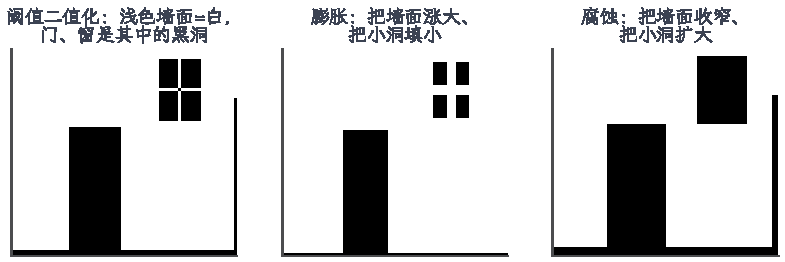
\includegraphics[width=0.95\textwidth]{figures/01-mathematical-preliminaries-upper/07-signals/matplotlib/teaching-signals-real-image/real-image-morphology.pdf}
  \caption{房屋墙面局部的形态学运算。左：阈值二值化后浅色墙面为白，深色门、窗是其中的洞；
  中：膨胀使白色区域涨大、小洞填小；右：腐蚀使白色区域收窄、小洞扩大。
  这些操作取邻域最大/最小，不是线性卷积。教学画面由脚本确定性生成。}
  \label{fig:real-image-morphology}
\end{figure*}

\Needspace{6\baselineskip}
\section{卷积映射的快速计算}
\label{sec:signal-analysis-fast-transforms}

\subsection{局部汇总的代价与五条计算路线}

前面的卷积映射在既定边界与存在条件下，由核$h$和输入决定，输出就是输入与$h$的卷积。
这个结论把“设计一个系统”化简成“设计一个核”，但它同时留下一个计算问题：
给定输入和核，怎样求出输出。这里的规模压力来自真实数据而不是抽象练习：
一段一分钟的音频在两万赫兹采样下有一百二十万个样本，一张中等大小的图像有数百万像素，
而图像滤波往往要在许多通道、许多核上重复同样的局部点积。
按定义直接求和，每个输出位置都要读遍核覆盖的全部输入，总乘加量与
“输出位置数$\times$核元素数”成正比。在常见设置下这个量级可达十亿次以上，
因此需要寻找复用了中间结果、或用更少乘法完成同样任务的算法。

卷积值得单独研究，不只因为它描述LTI系统。许多机器学习操作在形式上就是局部加权汇总：
图像上的平滑与边缘检测把每个像素邻域的亮度按核权重加起来；
一维序列上的移动平均用相邻若干项的加权和替换当前值；
处理序列的模型沿时间轴累积历史信息时，也大量使用这类按滞后加权的线性组合。
这些操作的共同结构是：输出某一点的取值只取决于输入在一个固定大小窗口内的值，
窗口逐点平移而权重不变。核与输入位置无关，这正是要利用的性质——
同一个小窗口反复出现，就有可能只算一次它的贡献，让多个输出共用。

不过“共用”不是无条件成立的，它取决于所求的输出范围。
按定义直接求完整线性卷积时，会枚举核元素与输入元素的全部配对乘积；
只求一个valid输出块时，直接算法可以略去不参与所需输出的乘积。
但这些只是直接算法的工作量，并不是任何算法都必须逐项支付的代价；
后面的求值与插值正是为了不单独计算每个原始乘积、仍恢复完整结果。
若索引本身是循环的，答案又变成循环卷积。三种目标的多项式表示不同，可用的加速手段也不同。
因此下面的比较都固定同一组输入和核，只改变计算过程，
避免把“换了目标”误当成“换了算法”。

\begin{table*}[htbp]
  \centering
  \begin{tabularx}{\linewidth}{@{}lXXX@{}}
    \toprule
    路线 & 朴素做法贵在哪里 & 改变的环节 & 代价出现在哪里\\
    \midrule
    直接求和 & 每个输出重算该窗口的全部乘积 & 无 & 乘加量随核元素数线性增长\\
    矩阵化 & 大量短点积逐个调用底层例程 & 只改变计算的组织形式 & 普通矩阵乘法不减少乘加，只是让库函数能统一优化\\
    FFT & 每个频率都要逐项积求和 & 改用频率坐标，把卷积变成逐点乘法 & 需要补零、复数运算与正反变换\\
    Toom--Cook & 全部乘积都当成独立乘法 & 用求值与插值替代高次系数乘法 & 增加求值、插值与常数除法，且会算出不需要的系数\\
    Winograd & 为每个输出重复同一套点积 & 固定小窗口的变换，只用一次小块乘法 & 变换矩阵的尺度差异会放大舍入误差\\
    空间可分离 & 二维核的乘法量是两轴长度之积 & 把二维核写成两个一维核的组合 & 只有核具有相应低秩结构时才成立\\
    \bottomrule
  \end{tabularx}
  \caption{同一卷积目标下五条计算路线的改动位置。每一条都回答“原来的哪一步贵”，
  因此它们可以在同一份输入上比较；选择哪一条还要结合核的大小、输出范围和数值精度要求。
  表中列出的是改动环节，不承诺某条路线在任意规模下都更快。}
  \label{tab:signal-analysis-fast-transform-roadmap}
\end{table*}

把卷积写成多项式乘法是上述比较的统一语言。多项式只是把数组的第$j$个位置记成幂次$z^j$、
把读数记成系数，并不引入新的数据，但它让“按位置汇总”变成“按幂次合并同类项”，
后文的取余、求值和插值都作用在这个多项式上。

先固定所求的是完整线性卷积、循环卷积，还是某个valid输出块，再比较计算路线。
对有限序列的多项式$X(z)=\sum_{i=0}^{m-1}x_i z^i$与
$H(z)=\sum_{j=0}^{r-1}h_jz^j$，乘积为
\begin{align}
  X(z)H(z)
  &=\sum_{i=0}^{m-1}\sum_{j=0}^{r-1}x_i h_jz^{i+j}\notag\\
  &=\sum_{n=0}^{m+r-2}\left(\sum_{i+j=n}x_i h_j\right)z^n.
  \label{eq:signal-analysis-polynomial-convolution}
\end{align}
系数恰为线性卷积，多项式的交换律与结合律也解释了有限卷积的相应性质。
贯穿例给出
\begin{equation}
  P(z)=(1+2z+z^2)(1-z)=1+z-z^2-z^3.
  \label{eq:signal-analysis-running-polynomial-product}
\end{equation}
循环边界则在乘积后取余：
\begin{equation}
  (XH)\bmod(z^N-1)=\sum_{n=0}^{N-1}(x*_Nh)[n]z^n,
  \label{eq:signal-analysis-polynomial-circular-convolution}
\end{equation}
这里$x,h$都以长度$N$编码，$z^{N+s}\equiv z^s$正好合并回绕项。
也就是说，次数达到或超过$N$的项没有消失，而是被折回到低次项上、与低次项相加。
这就是循环卷积的由来：它对应长度$N$的循环索引，而不是零延拓下的线性卷积。
当乘积次数小于$N$时无处可折、取模不改系数，两种结果才一致；
这也是“补零到长度至少$m+r-1$再做快速变换”能得到线性卷积的原因。
这些对应本身没有减少运算；还要选择能复用中间结果或减少核心乘法的计算过程。

直接求和枚举每个窗口中输入与核的全部乘积。下面比较如何把这些点积集中为矩阵乘法、
转换为点值或余数中的乘法，以及利用核的可分离结构。输入系数与核系数相乘记为核心乘法；
固定变换中的加减和常数乘法另行计入。核心乘法减少，不保证工作区或实际运行时间同时减少。

\subsection{基于矩阵乘法的卷积计算}\label{sec:signal-analysis-fast-matrix}
\label{sec:cnn-matrix-algorithm}

卷积定义里有一大批结构完全相同的短点积：每个输出位置对应一个窗口，
点积长度都是核元素数，只是取数起点平移了一格。
逐个写完这些点积并没有错，但每一次都很短，单独调用一次底层乘法例程时，
调用开销和地址计算会占掉大部分时间。已有的成熟优化都集中在矩阵乘法上，
其分块、向量化和多线程已经能把这部分硬件用好；
因此第一条路线并不减少乘加次数，而是把散落的小点积重新组织成一次大矩阵乘法，
以便直接使用这些实现。

对同一组输入窗口计算多个核的响应时，各个局部点积长度相同，可以集中交给
\term{通用矩阵乘法}（general matrix multiplication, GEMM）。
以下先取实值二维网格滤波，输入通道数为$c_{\mathrm{in}}$，核的两个轴长度为$k_h,k_w$。
从代数上把每个输入窗口展平成一列，得到$\bm P\in\mathbb R^{q\times n_{\mathrm{win}}}$；
这里$q=k_hk_wc_{\mathrm{in}}$为窗口元素数，$n_{\mathrm{win}}$为当前处理的窗口数，
与前文输入长度$m$区分。把每个输出核展平成一行，得到
$\bm W_{\mathrm{loc}}\in\mathbb R^{c_{\mathrm{out}}\times q}$。所有输出写成
\begin{equation}
  \bm Z_{\mathrm{col}}=\bm W_{\mathrm{loc}}\bm P\text{。}
  \label{eq:signal-analysis-window-matrix-product}
\end{equation}
其中$c_{\mathrm{out}}$为输出通道数。矩阵乘法后，把每个列索引还原为对应窗口的空间位置即可。
矩阵每一列对应一个空间窗口，每一行输出对应一个核；乘积中的第$(o,\ell)$个元素
正是第$o$个核与第$\ell$个窗口的点积。多输入通道不改变这个关系，只让每个窗口列更长；
多输出通道则让核矩阵增加行数。展开的元素顺序必须与核的展平顺序一致：
例如先遍历核行、核列再遍历通道，就不能把核按通道优先展平。

取二维输入和核
\begin{equation}
 \bm X=\begin{bmatrix}1&2&3&4\\5&6&7&8\\9&10&11&12\\13&14&15&16\end{bmatrix},
 \qquad \bm K=\begin{bmatrix}1&0\\0&-1\end{bmatrix}.
 \label{eq:signal-analysis-matrix-filter-example}
\end{equation}
这里计算valid互相关：每次窗口平移一格（步长一）；核读取相邻索引，不跳过中间位置，
也不填充输入。共有九个输出位置。按行优先排列窗口与窗口中的元素，有
\begin{equation}
  \bm P=\begin{bmatrix}
    1&2&3&5&6&7&9&10&11\\
    2&3&4&6&7&8&10&11&12\\
    5&6&7&9&10&11&13&14&15\\
    6&7&8&10&11&12&14&15&16
  \end{bmatrix}\text{，}
  \label{eq:cnn-im2col-example}
\end{equation}
核行为$(1,0,0,-1)$，矩阵乘积得到九个$-5$。例如前两列分别是
$(1,2,5,6)^\top$和$(2,3,6,7)^\top$，同一核行与它们相乘得到$1-6$与$2-7$，
图~\ref{fig:cnn-matrix-algorithm}给出对应关系。这种矩阵表示没有减少普通算法的
$c_{\mathrm{out}}q n_{\mathrm{win}}$次乘加，却把全部局部点积集中成同一个矩阵乘法。
$\bm P$可以是一个仅用于推导的逻辑矩阵，是否真的复制每个元素是存储实现的选择，
代数等式不要求保存整张窗口矩阵。


\begin{figure*}[htb]
  \centering
  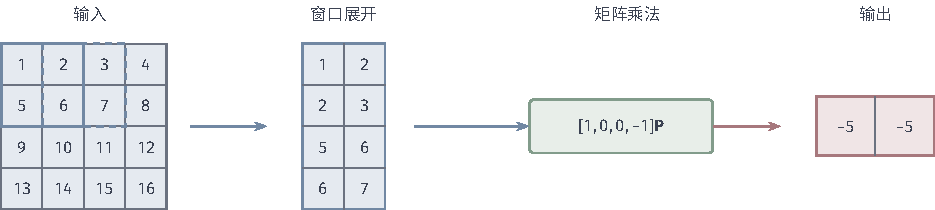
\includegraphics[width=158.358mm]{figures/01-mathematical-preliminaries-upper/07-signals/tikz/cnn-matrix-algorithm/figure.pdf}
  \caption{局部点积如何成为矩阵乘法。图中只取前两个相邻窗口，按核行、核列的顺序展平成$\bm P$的两列；
  核按相同顺序展平成一行。矩阵乘法同时得到这两个窗口的输出，完整计算包含九列。
  这里画的是代数上的窗口矩阵，是否实际复制全部数值由工程实现决定。}
  \label{fig:cnn-matrix-algorithm}
\end{figure*}
矩阵化之后还可以选择不同的矩阵乘法算法。下面的Strassen改变块乘法数量，
它从属于矩阵乘法这条计算路线，与是否显式保存窗口是两个问题。

\paragraph{Strassen递归乘法}
\label{sec:cnn-strassen}

先设$\bm A,\bm B$为同阶的$n\times n$方阵，$n$为偶数，且$\bm C=\bm A\bm B$。
把三个矩阵各划成$2\times2$个块，每块都是$(n/2)\times(n/2)$方阵，普通算法给出
\begin{equation}
  \begin{aligned}
    \bm C_{1,1}&=\bm A_{1,1}\bm B_{1,1}+\bm A_{1,2}\bm B_{2,1},\\
    \bm C_{1,2}&=\bm A_{1,1}\bm B_{1,2}+\bm A_{1,2}\bm B_{2,2},\\
    \bm C_{2,1}&=\bm A_{2,1}\bm B_{1,1}+\bm A_{2,2}\bm B_{2,1},\\
    \bm C_{2,2}&=\bm A_{2,1}\bm B_{1,2}+\bm A_{2,2}\bm B_{2,2}\text{。}
  \end{aligned}
  \label{eq:cnn-classical-block-product}
\end{equation}
四个输出各含两次块乘法，共需八次。Strassen算法用七个组合块乘积替代这八次乘法，定义
\begin{equation}
  \begin{aligned}
    \bm M_1&=(\bm A_{1,1}+\bm A_{2,2})(\bm B_{1,1}+\bm B_{2,2}),\\
    \bm M_2&=(\bm A_{2,1}+\bm A_{2,2})\bm B_{1,1},\\
    \bm M_3&=\bm A_{1,1}(\bm B_{1,2}-\bm B_{2,2}),\\
    \bm M_4&=\bm A_{2,2}(\bm B_{2,1}-\bm B_{1,1}),\\
    \bm M_5&=(\bm A_{1,1}+\bm A_{1,2})\bm B_{2,2},\\
    \bm M_6&=(\bm A_{2,1}-\bm A_{1,1})(\bm B_{1,1}+\bm B_{1,2}),\\
    \bm M_7&=(\bm A_{1,2}-\bm A_{2,2})(\bm B_{2,1}+\bm B_{2,2})\text{。}
  \end{aligned}
  \label{eq:cnn-strassen-products}
\end{equation}
由这些结果恢复输出：
\begin{equation}
  \begin{aligned}
    \bm C_{1,1}&=\bm M_1+\bm M_4-\bm M_5+\bm M_7,\\
    \bm C_{1,2}&=\bm M_3+\bm M_5,\qquad
    \bm C_{2,1}=\bm M_2+\bm M_4,\\
    \bm C_{2,2}&=\bm M_1-\bm M_2+\bm M_3+\bm M_6\text{。}
  \end{aligned}
  \label{eq:cnn-strassen-recovery}
\end{equation}
这种组合靠的是多余项的抵消，而不是省略某个输入块。以左上输出为例，把四个中间量按左因子归并，有
\begin{equation}
  \begin{aligned}
    \bm M_1+\bm M_4-\bm M_5+\bm M_7
    ={}&\bm A_{1,1}(\bm B_{1,1}+\bm B_{2,2}-\bm B_{2,2})\\
       &+\bm A_{1,2}(-\bm B_{2,2}+\bm B_{2,1}+\bm B_{2,2})\\
       &+\bm A_{2,2}(\bm B_{1,1}+\bm B_{2,2}+\bm B_{2,1})\\
       &-\bm A_{2,2}(\bm B_{1,1}+\bm B_{2,1}+\bm B_{2,2})\\
    ={}&\bm A_{1,1}\bm B_{1,1}+\bm A_{1,2}\bm B_{2,1}\text{。}
  \end{aligned}
  \label{eq:cnn-strassen-cancellation}
\end{equation}
展开过程没有交换左右因子，因而对矩阵块同样成立。其余三个输出也可按式~\eqref{eq:cnn-strassen-recovery}验证。核查例子取
\[
  \bm A=\begin{bmatrix}1&2\\3&4\end{bmatrix},\qquad
  \bm B=\begin{bmatrix}5&6\\7&8\end{bmatrix}\text{。}
\]
七个中间乘积依次为$65,35,-2,8,24,22,-30$，恢复后的结果是
$\left[\begin{smallmatrix}19&22\\43&50\end{smallmatrix}\right]$，与普通乘法一致。

这一层递归把八次块乘法降为七次，块加减却从四次增为十八次，其中十次用于形成乘法输入、
八次用于恢复输出。对$n\times n$方阵递归时，每个子问题的边长减半，
加减工作量仍与本层全部元素数成正比，因此$T(n)=7T(n/2)+O(n^2)$，
得到$O(n^{\log_2 7})$。指数降低来自每层少一个乘法子问题，
额外加减则是所支付的代价\scite{strassen1969}。

实现时通常只递归到合适阈值，底层仍调用高效GEMM；奇数尺寸需要拆分尾部或补齐，
临时块应复用，某些加减可并入数据打包。卷积可在
式~\eqref{eq:signal-analysis-window-matrix-product}的矩阵乘法阶段接入该算法，
但$c_{\mathrm{out}}\times q$与$q\times n_{\mathrm{win}}$常高度不对称，
盲目补成方阵会浪费大量工作。递归、额外加减与写回可能抵消节省；
相减还会改变舍入误差的传播。Strassen是一条可用的矩阵算法路线，
不能由渐近指数直接推出它适合每次网格滤波。

\subsection{基于傅里叶变换的卷积计算}\label{sec:signal-analysis-fast-fft}\label{sec:cnn-fft}

矩阵路线把短点积集中起来交给更高效的乘法，但乘加量本身没有下降。
要真正减少乘法，需要换一组坐标，让原来“把许多乘积加起来”的卷积变成数组之间对应位置直接相乘——
逐点相乘只需要$N$次，而不是$N^2$次。这正是前面频域表示的用处：
同一个循环卷积，在位置坐标下是多次平移的加权求和，在DFT坐标下则变为逐点相乘。
这背后的原因前面已经讲过：每个复指数都是平移的特征模式，一个卷积核作用在它上面
只是乘上一个常数（该频率的频率响应）；单次平移则只是与移位脉冲作循环卷积的特例。
上一节也已严格证明循环卷积在频率坐标下正是逐项相乘，核的DFT系数就是循环卷积算子的特征值。
整条路线于是分成三步：把输入和核都变换到频率域、逐点相乘、再反变换回来。
若每一步的DFT还要用定义逐项求和，这组三步比直接卷积更贵，
所以这条路线还依赖一项独立事实：DFT本身可以远快于定义式计算。

直接求$N$个DFT系数需要$O(N^2)$次运算，再调用卷积定理并不会自动提速。
\term{快速傅里叶变换}（fast Fourier transform, FFT）是一族快速计算DFT的算法，
并不是另一种频率变换。它省下运算的方式是让不同频率的计算共用中间结果：
先把序列按偶数位置和奇数位置分成两半，两半各自的变换长度减半，
再把它们组合出全部频率的系数。基二Cooley--Tukey分解利用偶数长度的单位根结构复用子结果，
正是这一做法\scite{cooley1965fft}。
令$x_{\mathrm e}[r]=x[2r]$、$x_{\mathrm o}[r]=x[2r+1]$，
它们的$N/2$点DFT为$E[k],O[k]$。因为$\omega_N^2=\omega_{N/2}$，
\[
  \widehat x[k]
  =\sum_{r=0}^{N/2-1}x[2r]\omega_{N/2}^{kr}
   +\omega_N^k\sum_{r=0}^{N/2-1}x[2r+1]\omega_{N/2}^{kr}.
\]
而$\omega_N^{N/2}=-1$，子变换以$N/2$为周期，所以对$0\leq k<N/2$有蝶形关系
\begin{align}
  \widehat x[k]&=E[k]+\omega_N^kO[k],\notag\\
  \widehat x[k+N/2]&=E[k]-\omega_N^kO[k].
  \label{eq:signal-analysis-fft-butterfly}
\end{align}
\BookEquationAliases{\label{eq:cnn-fft-butterfly}}
同一对中间结果产生两个频率，并没有舍弃后一半。
当$N=2^q$时，$T(N)=2T(N/2)+O(N)$，共$q$层、每层$O(N)$次运算，
所以复杂度为$O(N\log N)$。其他合数长度可按其他因子分解，质数长度也有相应算法；
补到二的幂只是某些实现的便利选择，不是FFT的普遍必要条件。

贯穿例补零到$N=4$，取$\bm x_4=(1,2,1,0)$、$\bm h_4=(1,-1,0,0)$。
$x_4$的偶分支$(1,1)$的二点DFT为$(2,0)$，奇分支$(2,0)$的为$(2,2)$。
用$\omega_4=-\mathrm i$合并得到
\[
  \widehat{\bm x}_4=(2+2,\ 0-2\mathrm i,\ 2-2,\ 0+2\mathrm i)
  =(4,-2\mathrm i,0,2\mathrm i).
\]
$h_4$的偶、奇分支DFT分别为$(1,1)$与$(-1,-1)$，同样得到
$\widehat{\bm h}_4=(0,1+\mathrm i,2,1-\mathrm i)$。
这一步显示如何复用两个二点变换，而不只是代入四点定义。
对$x_4$逆变换的四个分子依次为
\[
  4-2\mathrm i+2\mathrm i,\quad 4+2+2,\quad
  4+2\mathrm i-2\mathrm i,\quad 4-2-2,
\]
除以$4$后恢复$(1,2,1,0)$，同时核对了频率顺序、指数符号及归一化。
逐点乘积
$\widehat{\bm x}_4\odot\widehat{\bm h}_4=(0,2-2\mathrm i,0,2+2\mathrm i)$，
逆DFT给出$(1,1,-1,-1)$。若只用$N=3$，得到的是$(0,1,-1)$，
因为末项已经回绕；再精确的FFT也不能把这个循环输出当作原完整卷积。

\paragraph{长输入的分块计算}

对长输入作一次整体变换会占用较大工作区。FFT也可以逐块计算，以限制变换规模。
\term{重叠相加}（overlap-add）把输入分块，每块补零后计算完整线性卷积，再把重叠的输出贡献相加；
\term{重叠保留}（overlap-save）则让相邻输入块保留核长减一的重叠，只输出每块中
没有循环污染的部分。一维核长$k\geq1$、变换长度$N\geq k$时，每块可保留$N-k+1$个新输出。
例如把$(1,2,3,4)$拆为$(1,2)$与$(3,4)$，分别和$(1,-1)$作完整卷积，
得到$(1,1,-2)$与$(3,1,-4)$。第二块原本从位置二开始，恢复后也要平移两位；
重叠位置的$-2$与$3$相加，便得到整段输出$(1,1,1,1,-4)$，见图~\ref{fig:cnn-fft-blocks}。
每块内部仍须补零至至少$2+2-1=3$，分块不能消除线性卷积的补零要求。

重叠保留选择另一种组织方式。取核长二、$N=4$，每个输入块保留前一块最后一个输入值，
再接三个新值。首块为$(0,1,2,3)$，其循环卷积为$(-3,1,1,1)$；
丢掉受回绕污染的第一项，保留$(1,1,1)$。下一块为$(3,4,0,0)$，保留结果$(1,-4,0)$，
按目标长度截取前两项，仍恢复同一个完整输出。图~\ref{fig:cnn-fft-blocks}右侧把这一步与重叠相加并列。
重叠相加在输出端相加，重叠保留在输入端重叠并丢弃污染位置，两者不能混用拼接规则。

\begin{figure*}[htb]
  \centering
  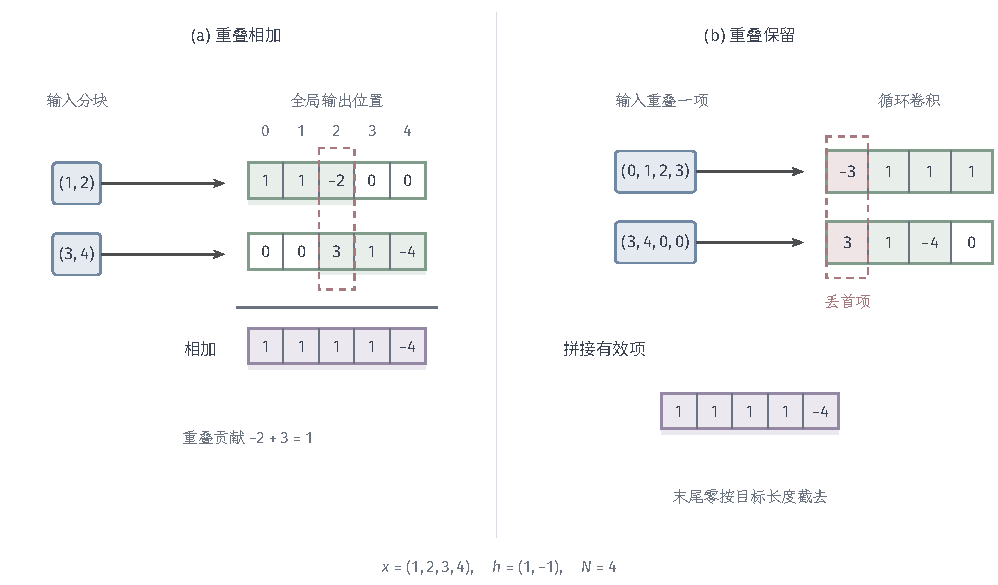
\includegraphics[width=168.998mm]{figures/01-mathematical-preliminaries-upper/07-signals/tikz/cnn-fft-blocks/figure.pdf}
  \caption{同一输入$(1,2,3,4)$与核$(1,-1)$的两种分块计算，均取$N=4$。
  左图把两个完整块卷积放回全局位置，红虚线框中的贡献$-2$与$3$相加为$1$。
  右图让相邻输入块重叠一项，丢弃红框中的循环污染首项，再拼接其余输出；
  末尾补零产生的多余输出按目标长度截去。两条计算链都恢复五项完整线性卷积，
  输出相加与污染项丢弃是不同的拼接规则。}
  \label{fig:cnn-fft-blocks}
\end{figure*}

块太小会使变换和重叠的开销增加，块太大则增加内存及延迟。
复数数组、变换代价与跨步后被丢弃的输出，都会影响分块是否减少总耗时。

\subsection{基于多项式插值的卷积计算}\label{sec:signal-analysis-fast-toom}\label{sec:cnn-toom-cook}

FFT用单位根这一组特殊选点换取快速变换，代价是要引入复数、并对序列长度有要求。
回到多项式乘法还能看出一个更一般的道理：减少乘法的关键并不是非选单位根不可，
而是利用“求值”和“乘法”可以交换顺序。直接相乘时，$(a+bz)(c+dz)$要做四次小乘法
再合并同类项；但如果先在几个点上分别求出两个多项式的值（求值只是加减），
把同一处的两个值相乘，再由这些乘积反推出系数（插值），所用的小乘法可以更少。
其根据是一条很朴素的性质：乘积多项式在任一点的值，等于两个原多项式在该点的值相乘——
$(X\cdot K)(a)=X(a)\cdot K(a)$，所以“先求值再相乘”和“先相乘再求值”结果一致。
这条路线的优势是选点自由，因而能针对小核、整数系数或短输出块作具体设计；
代价是求值和插值要额外做不少加减法，恢复过程也得另行求解。

Toom--Cook方法对多项式分块、求值、逐点相乘，再插值恢复系数。
先取输入$X(z)=x_0+x_1z$与核$K(z)=k_0+k_1z$。这两个次数至多为一的多项式可用
$0,1,\infty$三个坐标相乘，其中$\infty$表示读取约定的最高幂次位置的系数，
这里分别是$x_1$与$k_1$，允许为零。令$m_0=x_0k_0$、$m_\infty=x_1k_1$、
$m_1=(x_0+x_1)(k_0+k_1)$，则
\begin{equation}
  (x_0+x_1z)(k_0+k_1z)
  =m_0+(m_1-m_0-m_\infty)z+m_\infty z^2\text{。}
  \label{eq:cnn-toom-example}
\end{equation}
中间系数本来是$x_0k_1+x_1k_0$，现在通过一次组合乘法减去两端乘积得到。
四次数据与核之间的乘法降为三次；这个最小例子也称Karatsuba乘法。
例如$\bm x=(1,2)$、$\bm k=(1,-1)$时，三个乘积为$1,0,-2$，恢复得到系数$(1,1,-2)$。


这一组合乘法也可用于更多系数。对次数至多为二的$X$与次数至多为一的$H$，
乘积次数至多为$3$，可使用$0,1,-1,\infty$四个坐标；其中“无穷点”表示读取约定的
最高幂次位置的系数，不是把无穷大传给数值程序\scite{math-knuth1997seminumerical}。
记
\begin{align}
  r_0&=X(0)H(0),&r_+&=X(1)H(1),\notag\\
  r_-&=X(-1)H(-1),&r_\infty&=x_2h_1.\label{eq:cnn-toom-three-two-evaluation}
\end{align}
设$P(z)=c_0+c_1z+c_2z^2+c_3z^3$，
则$r_+=c_0+c_1+c_2+c_3$，$r_-=c_0-c_1+c_2-c_3$，
和、差分别解出偶次与奇次部分：
\begin{align}
  c_0&=r_0,\qquad c_3=r_\infty,\notag\\
  c_1&=\frac{r_+-r_-}{2}-c_3,\notag\\
  c_2&=\frac{r_++r_-}{2}-c_0.
  \label{eq:signal-analysis-toom-reconstruction}
\end{align}
\BookEquationAliases{\label{eq:cnn-toom-three-two-recovery}}
这是前述插值思想在包含最高次坐标时的具体形式；分母$2$要求系数域中$2$可逆。

贯穿例的四个值为$(r_0,r_+,r_-,r_\infty)=(1,0,0,-1)$，
恢复为$(c_0,c_1,c_2,c_3)=(1,1,-1,-1)$。
直接展开需$3\times2=6$次输入系数与核系数相乘，此方案只需四次点值乘法，
却增加了求值、插值及常数乘除。长多项式可递归分块获得渐近改进，
短核则未必值得；缓存、数据变换和访存也要计入。
点值乘法之所以成立，是因为$P(a)=X(a)H(a)$，而不是因为任意坐标变换都把乘法变成逐点乘法。

\paragraph{三段分块与递归}

三段分块进一步展示插值过程。对两个次数至多为二的多项式，在$0,1,-1,2,\infty$求值并相乘，
记结果为$r_0,r_1,r_{-1},r_2,r_\infty$。这里使用实数或复数系数，除以$2$和$3$都有定义；
其他系数域须检查二者是否可逆。乘积次数至多为四，正好需要五个条件：
$c_0,c_4$由两端直接给出；$r_1+r_{-1}$分离偶数次项，$r_1-r_{-1}$给出$c_1+c_3$；
再用$r_2$区分这两个奇数次系数。乘积系数$c_0,\ldots,c_4$可按下式恢复：
\begin{equation}
  \begin{aligned}
    c_0&=r_0,\qquad c_4=r_\infty,\\
    c_2&=(r_1+r_{-1})/2-c_0-c_4,\\
    v&=(r_1-r_{-1})/2,\\
    u&=(r_2-c_0-4c_2-16c_4)/2,\\
    c_3&=(u-v)/3,\qquad c_1=v-c_3\text{。}
  \end{aligned}
  \label{eq:cnn-toom-three}
\end{equation}
这里$u,v$只是插值中间量。五次求值后的乘法替代九次原始系数乘法，但新增了求值加减、
常数乘除和插值。例如$\bm x=(1,2,3)$、$\bm k=(1,-1,2)$的五个点值乘积是
$1,12,8,119,6$；式~\eqref{eq:cnn-toom-three}先给出$c_2=3,v=2,u=5$，
再得到$c_3=1,c_1=1$，完整输出为$(1,1,3,1,6)$。

长序列可以每$\ell$项分为一段，写成$X(z)=X_0(z)+z^\ell X_1(z)+z^{2\ell}X_2(z)$，
核也同样分段。把$z^\ell$暂看成外层变量，刚才的五次乘法就变为五个短多项式乘法；
每个段内乘积再递归计算。插值后将第$j$个段内结果平移$j\ell$位，并把重叠系数相加。
对两条长度相近的序列，三等分递归满足$T(n)=5T(n/3)+O(n)$，
理想成本为$O(n^{\log_3 5})$；它不能直接作为长输入与短滤波核的复杂度，
因为两者形状并不相近。

实现时需选择分块长度和求值点，保存或流式产生求值结果，并把恢复的系数按原位置累加。
求值点过大、或插值中出现相近量相减，可能放大浮点误差；低精度下尤其要检查变换后的动态范围。
数学卷积与互相关可通过共轭反转核及相应输出选段建立对应，但局部滤波通常只需一小段输出，
计算完整多项式乘积可能浪费工作。Toom--Cook解释了“用变换交换乘法与加法”的一般思路，
接下来的Winograd则直接面向小块滤波输出。

\subsection{基于余数分解的卷积计算}\label{sec:signal-analysis-fast-winograd}\label{sec:cnn-winograd}

Toom--Cook按次数界选择一组点，恢复的是整条乘积的全部系数。
实际滤波有时只需要少数几个相邻输出，算出完整乘积会浪费大半工作，
而且不同输出块的恢复公式还得分别推导。
上一小节建立的多项式工具提供了另一条出路：把多项式换成关于几个低次模的余数，
在这些余数上相乘，再用中国剩余定理拼回去。
余数比点值自由，因为模不限于一次多项式；若模是一次多项式，余数就是一个数，
这一路线便退化为点值插值。当任务只要一小块输出时，可以选择只恢复所需系数的那组模，
从而在减少乘法的同时避免算不需要的部分。

Winograd类算法据此构造乘法较少的乘积或滤波计算，特定输出块还需相应的恢复映射
\scite{math-winograd1980arithmetic}。
回到贯穿例，令$X(z)=1+2z+z^2$、$H(z)=1-z$，
完整乘积仍为$P(z)=X(z)H(z)=1+z-z^2-z^3$。先取
$M(z)=z^4-1=(z-1)(z+1)(z^2+1)$。
三个实系数因子两两互素、总次数为$4$，分别有
\[
  P(1)=0,\quad P(-1)=0,\qquad
  X\bmod(z^2+1)=2z,\quad H\bmod(z^2+1)=1-z.
\]
在第三个模下$z^2=-1$，所以$XH\equiv2+2z$。
设恢复的$R$次数小于$4$，前两份零余数使
$R(z)=(z^2-1)(az+b)$。再模$z^2+1$得到$R\equiv-2az-2b$，
与$2+2z$比较便有$a=b=-1$，从而$R=1+z-z^2-z^3$。
原乘积次数已经小于$4$，因此这正是完整乘积；若次数更高，就只能得到模代表元。
本次映射从长度$3$和$2$的输入恢复四项完整卷积，不能直接称作任意输出块的最小算法。

回到长度三与长度二的乘积，沿用式~\eqref{eq:cnn-toom-three-two-evaluation}，
选取$z,z-1,z+1$，其乘积为$M(z)=z^3-z$。用$S$记
式~\eqref{eq:signal-analysis-toom-reconstruction}所恢复的乘积。
由于$S$次数至多为三、最高次项系数是$r_\infty$，可写成
\begin{equation}
  S(z)=r_\infty M(z)+R(z),\qquad \deg R<3\text{。}
  \label{eq:cnn-winograd-polynomial-remainder}
\end{equation}
在$0,1,-1$处$M$都为零，故$R$保留$S$在这三点的值$r_0,r_+,r_-$。
下面三个二次多项式各自在一个点等于一、在另外两点等于零：
\[
  L_0(z)=1-z^2,\quad
  L_+(z)=(z^2+z)/2,\quad
  L_-(z)=(z^2-z)/2\text{。}
\]
因而余数的具体重构式是
\begin{equation}
  R(z)=r_0L_0(z)+r_+L_+(z)+r_-L_-(z)\text{。}
  \label{eq:cnn-winograd-remainder-reconstruction}
\end{equation}
代入并展开$r_\infty(z^3-z)+R(z)$，就得到式~\eqref{eq:cnn-toom-three-two-recovery}的四项系数。
该例中一次基多项式的余数就是点值，所以余数重构与Toom--Cook插值给出同一个计算过程；
选择更一般的基多项式时，余数也可能是低次多项式，而非一个数值。

\paragraph{从完整卷积转为小块滤波}

上面用余数恢复的是整条卷积的全部系数。但卷积网络实际做互相关时，常常只需要窗口完全落在
输入内的那几个相邻输出，算出完整卷积会多做无用功。这里有一个巧妙的转换：
“用固定核去卷积”是个线性映射，可以写成矩阵；把这个矩阵转置，完整卷积的计算图就变成
小块互相关的计算图，而所用的核心乘法次数不变。先看这个对应关系：
固定长度三的实核$\bm g=(g_0,g_1,g_2)^\top$，把它与长度二的实向量$\bm b$作完整数学卷积，
可写为$\bm s=\bm H_{\bm g}\bm b$，其中
\begin{equation}
  \bm H_{\bm g}=\begin{bmatrix}
    g_0&0\\g_1&g_0\\g_2&g_1\\0&g_2
  \end{bmatrix},\qquad
  \bm H_{\bm g}^\top\bm d=
  \begin{bmatrix}
    d_0g_0+d_1g_1+d_2g_2\\
    d_1g_0+d_2g_1+d_3g_2
  \end{bmatrix}\text{。}
  \label{eq:cnn-winograd-filter-transposition}
\end{equation}
右侧正是长度四的实输入$\bm d$经过该核产生的两个相邻互相关输出（也就是网络里一个$3$长核
在$4$个输入上步长$1$滑动得到的两个valid结果）。把前面完整卷积的线性计算图整体转置，
就可以把“长度二输入、四个完整输出”的问题变成“长度四输入、两个有效输出”的问题，
核心乘法仍是四次，一次都不必增加。

更具体地，若完整卷积算法写为$\bm s=\bm R[(\bm E\bm g)\odot(\bm Q\bm b)]$，
其中$\bm E,\bm Q$负责求值、$\bm R$负责恢复，则固定核后整个映射是
$\bm R\operatorname{Diag}(\bm E\bm g)\bm Q$。转置后得到
\[
  \bm H_{\bm g}^\top\bm d
    =\bm Q^\top[(\bm E\bm g)\odot(\bm R^\top\bm d)]\text{。}
\]
这里$\operatorname{Diag}$把向量放到对角线上；转置只反转线性变换的顺序，
逐项乘法仍使用相同的四个核组合。把固定系数$1/2$在数据变换与核变换之间重新分配，
就得到下面常用的公式。整个构造依赖转置的乘积规则，不要求输入或输出变换可逆。

下面用记号$F(p,r)$表示：用一个$r$项的核，一次算出$p$个相邻的valid互相关输出，
为此需要$p+r-1$个连续输入。例如$F(2,3)$就是用$3$项核、读$4$个输入、产出$2$个输出。

\begin{example}[可复核的Winograd \(F(2,3)\)输出块]
  \label{ex:signal-analysis-winograd-f23}
  先把要算的东西直接写出来：固定一维valid互相关，输入$\bm d=(d_0,d_1,d_2,d_3)^\top$，
  核$\bm g=(g_0,g_1,g_2)^\top$，所需的两个输出只是
  \begin{align*}
    y_0&=d_0g_0+d_1g_1+d_2g_2,\\
    y_1&=d_1g_0+d_2g_1+d_3g_2.
  \end{align*}
  直接算要$6$次乘法。Winograd的$F(2,3)$改用关于$z,z-1,z+1$的余数与最高次系数坐标，
  核侧是$0,1,-1$处点值及最高次系数的缩放；
  输入侧则针对只恢复两项输出另作线性组合。一组符合本章方向约定的变换为
  \begin{equation}
    \bm y=\bm A^\top\bigl[(\bm G\bm g)\odot(\bm B^\top\bm d)\bigr],
    \label{eq:signal-analysis-winograd-f23}
  \end{equation}
\BookEquationAliases{\label{eq:cnn-winograd-matrix-a}
\label{eq:cnn-winograd-matrices-bg}
\label{eq:cnn-winograd-recovery-principle}
\label{eq:cnn-winograd-one-dimensional}
\label{eq:cnn-winograd-vector-transform}}
  其中
  \begin{align*}
    \bm B^\top&=\begin{bmatrix}
      1&0&-1&0\\0&1&1&0\\0&-1&1&0\\0&1&0&-1
    \end{bmatrix},\\
    \bm G&=\begin{bmatrix}
      1&0&0\\1/2&1/2&1/2\\1/2&-1/2&1/2\\0&0&1
    \end{bmatrix},\\
    \bm A^\top&=\begin{bmatrix}1&1&1&0\\0&1&-1&-1\end{bmatrix}.
  \end{align*}
  形状分别为$\mathbb R^4\to\mathbb R^4$、$\mathbb R^3\to\mathbb R^4$，
  逐点相乘后由$\mathbb R^4\to\mathbb R^2$恢复指定输出。
  为直接核对恒等式，记
  \begin{align*}
    m_1&=(d_0-d_2)g_0,\\
    m_2&=\tfrac12(d_1+d_2)(g_0+g_1+g_2),\\
    m_3&=\tfrac12(-d_1+d_2)(g_0-g_1+g_2),\\
    m_4&=(d_1-d_3)g_2.
  \end{align*}
  则$m_2+m_3=d_2g_0+d_1g_1+d_2g_2$，
  $m_2-m_3=d_1g_0+d_2g_1+d_1g_2$，
  所以$m_1+m_2+m_3=y_0$、$m_2-m_3-m_4=y_1$。

图~\ref{fig:cnn-winograd-example}取$\bm d=(1,2,3,4)$、$\bm g=(1,2,3)$，
得到$\bm m=(-2,15,1,-6)$，再恢复$(14,20)$；直接计算也给出
$1+4+9=14$和$2+6+12=20$。输入变换需要四次加减，核变换可用三次加减与两次乘以$1/2$，
输出恢复需要四次加减。含$1/2$的核变换在核系数不变时可复用，不应把全部变换开销计为零。


\end{example}

\begin{figure*}[htb]
  \centering
  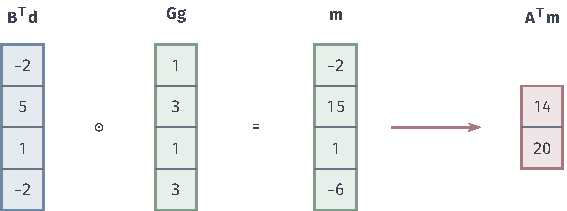
\includegraphics[width=95.934mm]{figures/01-mathematical-preliminaries-upper/07-signals/tikz/cnn-winograd-example/figure.pdf}
  \caption{一维$F(2,3)$的完整数值路径。输入$\bm d=(1,2,3,4)^\top$与核$\bm g=(1,2,3)^\top$
  分别变为四个组合值，按位置相乘得到$\bm m=(-2,15,1,-6)^\top$，再用输出变换恢复两个互相关结果。
  四次核心乘法替代直接算法的六次乘法，加减与固定系数变换仍有成本。}
  \label{fig:cnn-winograd-example}
\end{figure*}

\paragraph{沿两个轴组合变换}

图像卷积是二维的，而一维Winograd的好处可以沿行、列两个方向各用一次：对$3\times3$核和
$4\times4$输入块，先把核和输入分别用同一组矩阵沿两个轴变换，得到的逐元素乘积再恢复成
$2\times2$的四个输出：
\begin{equation}
  \begin{aligned}
    \bm U&=\bm G\bm K\bm G^\top,\qquad
    \bm V=\bm B^\top\bm D\bm B,\\
    \bm Y&=\bm A^\top(\bm U\odot\bm V)\bm A\text{。}
  \end{aligned}
  \label{eq:cnn-winograd-transform}
\end{equation}
左乘组合第一索引轴上的值，右乘组合第二索引轴上的值；因此$\bm U,\bm V$都是$4\times4$，
逐元素乘积有十六项，输出恢复把它变为$2\times2$。这不是对每个输出独立使用一维技巧，
而是两轴都先形成组合，再让十六个乘积服务于全部四个输出。直接计算的$4\times9=36$次
核心乘法降为$16$次\scite{lavin2016fast}。

这些矩阵对应步长一、核读取间隔为一的$3\times3$核；改变读取规则时必须重新构造变换。
核侧和输入侧的十六项变换值也要占用工作区，减少核心乘法并未免去变换成本。

\subsection{基于核分离的卷积计算}\label{sec:signal-analysis-fast-separable}
\label{sec:cnn-separable-implementation}

前面的路线从两个方面改变计算：矩阵化重新组织点积，并不减少普通乘加次数；
FFT、Toom--Cook与Winograd则在各自指定的输出范围和构造条件下，
利用变换减少核心乘法，同时付出变换与恢复的代价。
还有一类加速利用的是核自身的代数结构：二维卷积之所以往往昂贵，
是因为核在两个轴上的长度相乘（一个$3\times3$核每个输出要做$9$次乘法）。
但很多常见核——例如高斯模糊、Sobel边缘核——可以拆成“先横向、再纵向”两个小核，
$9$次于是降到约$3+3$次。能用的条件是二维核$k_{a,b}$恰好写成
一个列向量$u_a$与一个行向量$v_b$的乘积$u_av_b$；这时二维加权求和就能拆成两个方向的
一维加权求和，让第一轴算出的中间结果被第二轴上的多个输出复用，
乘法量从两轴长度之积降到两轴长度之和。核是否具有这种结构由任务决定，不是算法能选择的；
它成立时可以直接沿两轴先后滤波，不必先做频域变换，但边界补值仍须与原二维滤波一致。
实际能节省多少，要比较两次一维滤波的输出范围、中间数组和核长度，
不能仅凭可分离就断言它总比其他路线快。

若单通道核可写成$k_{a,b}=u_a v_b$，即$\bm K=\bm u\bm v^\top$，
二维滤波就可分解为一个方向长度$k_h$的滤波和另一个方向长度$k_w$的滤波。
这一分解直接来自求和顺序：
\begin{equation}
  \begin{aligned}
    t_{i,j}&=\sum_{b=0}^{k_w-1}v_bx_{i,j+b},\\
    y_{i,j}&=\sum_{a=0}^{k_h-1}u_at_{i+a,j}
      =\sum_{a=0}^{k_h-1}\sum_{b=0}^{k_w-1}
          u_av_bx_{i+a,j+b}\text{。}
  \end{aligned}
  \label{eq:cnn-spatial-separable-derivation}
\end{equation}
水平结果$t_{i,j}$可以被多个垂直窗口复用，因此不必为每个二维窗口重新计算整组水平点积。
窗口逐格移动、核读取相邻索引且逐轴边界与裁剪一致时，在足够大的网格上，
主要成本由每个输出附近的$k_hk_w$项降为约$k_h+k_w$项，代价是保存或流式处理一维中间结果。

取$\bm u=\bm v=(1,2,1)^\top$，则
$\bm K=\left[\begin{smallmatrix}1&2&1\\2&4&2\\1&2&1\end{smallmatrix}\right]$。
对式~\eqref{eq:signal-analysis-matrix-filter-example}中的$4\times4$输入，
水平滤波先得到$4\times2$的中间矩阵，再垂直滤波得到$2\times2$输出，
图~\ref{fig:cnn-spatial-separable}列出全部数值。左上输出为
$8+2\times24+40=96$，与直接二维求和一致。

这个小例子也提醒我们区分局部估算与完整成本。设输入大小为$h\times w$且
$h\geq k_h$、$w\geq k_w$，不填充且窗口逐格移动时，输出大小为
$h'=h-k_h+1$、$w'=w-k_w+1$，中间矩阵尺寸是$h\times w'$，
所以两阶段共需$hw'k_w+h'w'k_h$次核心乘法，并不严格等于$h'w'(k_h+k_w)$。
本例需要$4\times2\times3+2\times2\times3=36$次，与直接计算的
$2\times2\times9=36$次相同；对$100\times100$输入，同一核的两阶段成本为$58212$次，
直接计算则为$86436$次。图像相对核越大，中间区域的额外边界开销越容易摊薄。
\begin{figure*}[htb]
  \centering
  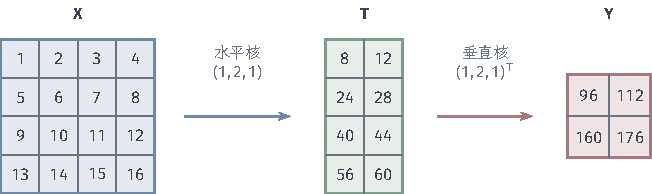
\includegraphics[width=110.335mm]{figures/01-mathematical-preliminaries-upper/07-signals/tikz/cnn-spatial-separable/figure.pdf}
  \caption{秩一空间核的两阶段计算。水平核与垂直核均为$(1,2,1)$，组成$3\times3$核$\bm u\bm v^\top$。
  在步长一、无填充条件下，原$4\times4$输入先变为$4\times2$中间结果，再变为$2\times2$输出。
  这个小例子的两阶段核心乘法量仍为三十六次，图示验证的是结果等价，而非每种输入尺寸都能节省计算。}
  \label{fig:cnn-spatial-separable}
\end{figure*}


一般核未必秩一。对核作奇异值分解，把第$r$个奇异值吸收到一个向量中，得到
$\bm K_\rho=\sum_{r=1}^{\rho}\bm u_r\bm v_r^\top$，其中$\rho$为保留的非零奇异值个数。
保留全部非零奇异值时$\bm K_\rho=\bm K$；计算$\rho$组一维滤波并相加，即可恢复原二维核的输出。
在大网格上每位置主要成本约为$\rho(k_h+k_w)$，只有它比$k_hk_w$足够小，
才可能抵消分解与中间读写。只保留较少奇异值通常会改变输出，属于近似算法，应检查输出误差。
这里分解的是单个空间核的两个轴，没有改变输入通道和输出通道之间的连接关系。

\begin{table*}[htb]
  \centering
  \begin{tabularx}{\linewidth}{@{}lXX@{}}
    \toprule
    计算路线 & 计算过程的改变 & 适用条件与代价\\
    \midrule
    直接计算 & 枚举全部局部乘积并累积 & 适用各种采样设置，乘加量为窗口数、窗口长度与输出通道数的乘积\\
    矩阵化计算 & 将点积集中为矩阵乘法 & 普通GEMM保持乘加量；Strassen可减少块乘法，但增加加减与误差敏感性\\
    Toom--Cook & 求值、逐点乘法、插值 & 面向多项式乘积，可能计算不需要的输出系数\\
    Winograd & 固定变换恢复小块滤波输出 & 小核、小步长设置；变换成本及数值条件需核对\\
    FFT & 频域乘法后反变换 & 线性卷积须补零，变换与复数运算有成本\\
    空间可分离核 & 低秩分解为一维滤波 & 无损计算要求相应低秩结构；截断分解会改变输出\\
    \bottomrule
  \end{tabularx}
  \caption{按计算过程比较卷积算法。矩阵化本身不减少普通乘加量，但提供了选择矩阵乘法算法的入口。
  前五条路线在精确算术下、满足各自边界与输出条件时恢复指定的卷积或互相关；
  空间可分离路线还要求核具有相应结构。表中不把显式展开、隐式取数等存储选择作为新的代数算法。}
  \label{tab:cnn-algorithms}\label{tab:signal-analysis-convolution-algorithms}
\end{table*}

图~\ref{fig:cnn-transform-algorithms}把三类变换放在同一条输入、乘法和恢复路径上；
它们的区别在于坐标选择与要恢复的输出。
\begin{figure*}[tb]
  \centering
  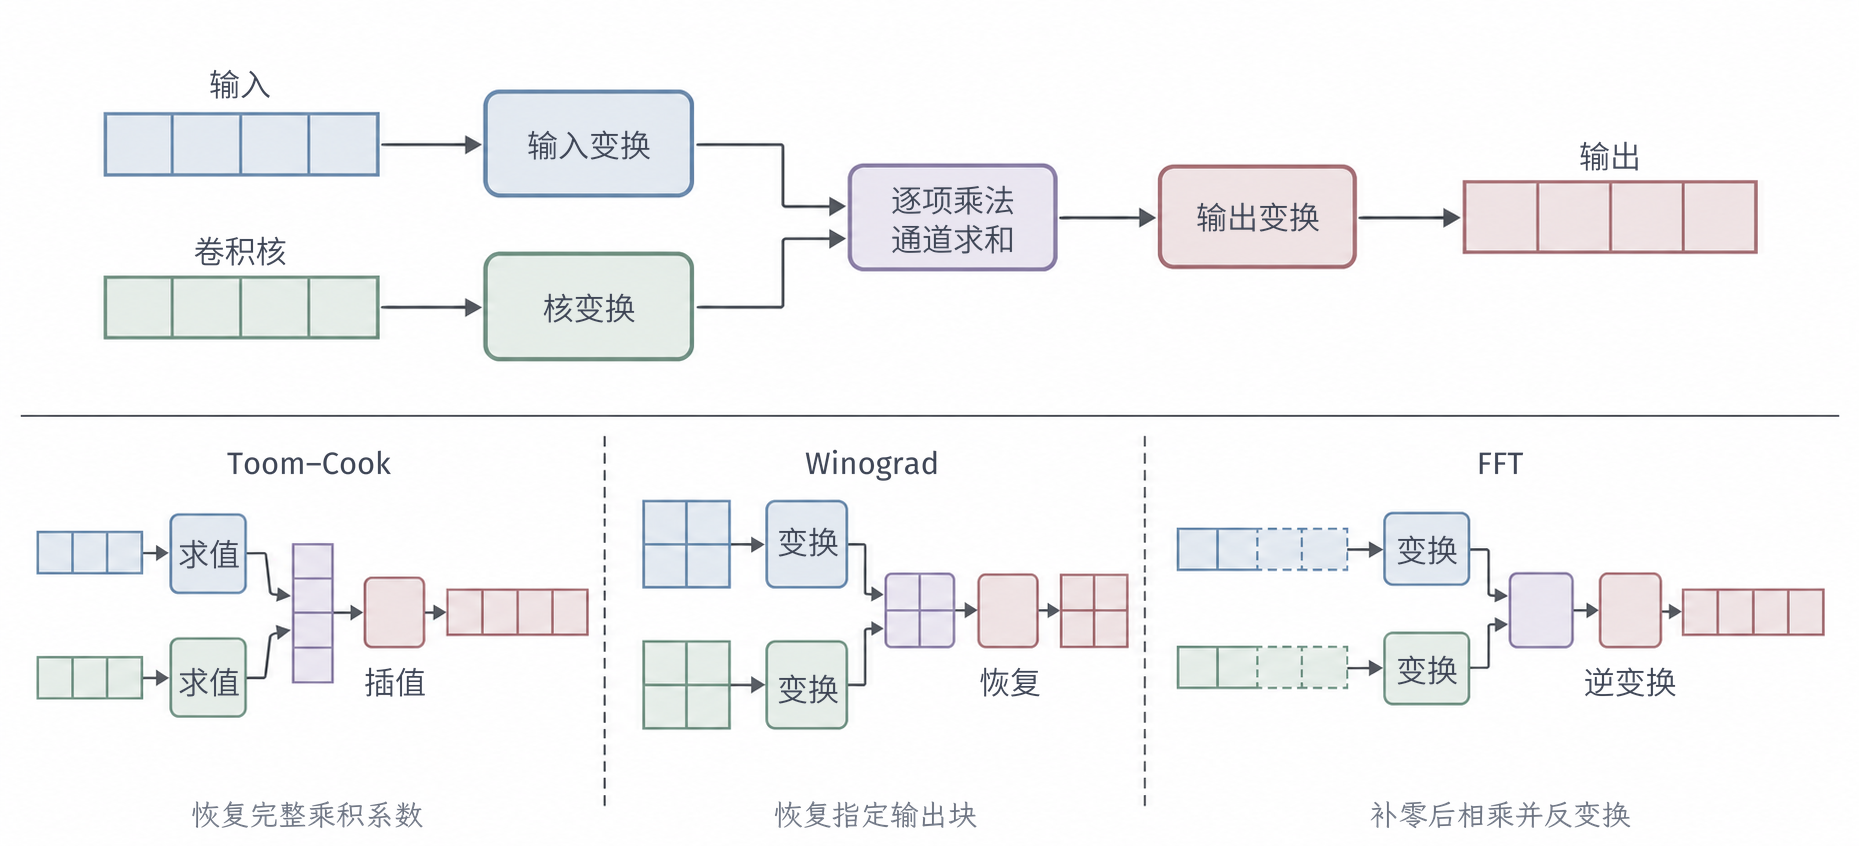
\includegraphics[width=169mm]{figures/01-mathematical-preliminaries-upper/07-signals/generated/cnn-transform-algorithms/figure.png}
  \caption{变换类卷积的共同流程与不同目标。Toom--Cook通过多项式求值及插值恢复完整乘积系数；
  Winograd通过固定小矩阵恢复所需输出块；FFT在补零后的频域相乘并反变换。
  输入和核可以分别变换，变换结果按输入通道相乘并求和；能复用多少次，决定变换开销能否被摊薄。
  格子只示意数组，不表示具体尺寸或数值。}
  \label{fig:cnn-transform-algorithms}
\end{figure*}

矩阵路线把窗口点积汇集为一个乘法；三类变换路线利用与乘法相容的表示，结构却不同。
FFT在$z^N-1$的全部复单位根处求值，并利用根的规则结构快速变换；
Toom--Cook允许一般选点及递归分块；Winograd类构造用互素余数，常针对指定的小块输出。
一次因子的CRT与点值插值重合，高次因子保留的却是一个低次多项式，不能称为单个点值。

长度相近的两个$n$项序列直接卷积需要$O(n^2)$次乘加，
FFT路线在合适长度上需$O(N\log N)$变换运算及$N$次频域乘法。
乘法数和渐近量级并非完整运行时间：加减、复数算术、常数运算、缓存复用与目标硬件
都会改变实际排序。归一化DFT是酉变换、条件良好，但多层蝶形仍会累积舍入误差；
Toom--Cook和Winograd的变换矩阵可能有较大尺度差异，相近量相减也会放大相对误差。

整数或有限域算法还要检查系数域条件。一个有限域（finite field）的例子是
模素数$p$的数系：只保留$0,\ldots,p-1$，加乘后取模，非零元素都有乘法逆元。
例如模$5$时$2\cdot3=1$，所以除以$2$就是乘以$3$。
数论变换（number-theoretic transform, NTT）在这类数系中按DFT的形式求值；
它需要有所需阶数的单位根，逆变换中的$N$也须可逆。
若$p$整除$N$，$N$在该数系中就是零，不能作为除数；
前面Toom--Cook的除以$2$、$3$也有同样的系数域限制。

若目标是恢复整数系数，还要从有限域运算返回整数余数重构。
此处的模数是整数，与前面的模多项式不同。设总整数模数为$Q$
（使用多个两两互素模数时取它们的乘积），选取区间$(-Q/2,Q/2]$内的余数代表。
已知每个真实系数绝对值不超过$B$时，$Q>2B$保证该代表唯一等于真实系数：
两个候选系数之差绝对值至多$2B$，不可能是非零的$Q$倍数。
第$n$个卷积系数的绝对值可由$\sum_{i+j=n}|x_i h_j|$控制，
再对输出位置取统一上界即可选取$B$。
避免浮点误差并不等于避免模混淆或整数溢出。
不存在脱离规模、数据类型和误差目标的普遍最优算法。

选择计算路线以后，还要核对它是否输出了所要求的映射。FFT计算完整线性卷积需要
足够补零；Toom--Cook恢复所设多项式乘积；互相关需要匹配核方向；Winograd恢复
构造时指定的小块输出。步长、核读取间隔或边界改变后，相应变换也要重新验证。
快速算法改变的是计算组织，输入与输出的含义仍由原问题确定。

\section{信号的采样与恢复}
\label{sec:signal-analysis-sampling}

前面各节都假定数据已经是数组，关心的是怎样表示和计算它。
但设备实际存下来的也正是数组：传感器按固定间隔读出数值，连续记录被压缩成一串有限精度的样本。
这里有一个容易被“DFT可以精确还原数组”掩盖的问题：
若日后需要重建样本之间的取值、或改变采样间隔，就要问清楚这一步转换究竟丢失了什么。
前面已经看到，DFT用同样多的频率坐标替换数组，保留全部坐标便能精确还原每一项；
但这个结论容易被误读成“采样本身也没有损失”。两者的对象不同：
坐标换法可逆，说的是数组与它的频率系数一一对应；
而原始连续信号在样本之间的取值从未进入数组，逆变换自然也无法仅凭数组把它们恢复出来。

要把这一步说清楚，最好先找一个具体的失败例子，看两条明显不同的连续信号
怎样产生同一串样本。这也是理解后面全部结论的钥匙：采样本质上是把连续信号
在等间隔点上的取值“抄录”成数组，抄录本身是多对一的——除非先限定被抄录的信号类别。
有了反例，再问需要补充什么条件才能排除它，这个条件就是后文的带限假设。
限制频率能保证恢复，但设备往往在采样前就已先把高频压低，这又改变了需要恢复的对象，
所以还要单独讨论这一步预滤波做了什么。这些一维关系建立之后，
再检查多维与时空格上的频率歧义，最后把插零和插值分开，说明增加数组位置为何不等于增加观测。

\subsection{采样后的频率混叠}
\label{sec:signal-sampling-ambiguity}

固定时间原点及采样间隔$T_s>0$，对具有确定点值的连续时间信号$f$读取
$x[n]=f(nT_s)$，采样频率为$\nu_s=1/T_s$。若不约束候选信号，采样通常不是单射。
例如$T_s=1$时，$f_1(t)=\cos(0.8\pi t)$与$f_2(t)=\cos(1.2\pi t)$频率不同，却满足
\[
  f_2(n)=\cos(2\pi n-0.8\pi n)=\cos(0.8\pi n)=f_1(n),
  \qquad n\in\mathbb Z.
\]
这就是\term{混叠}（aliasing）：不同的连续振荡在样本上无法区分。
图~\ref{fig:signal-aliasing-curves}中的两条曲线在样本之间起伏不同，
但每个整数位置都穿过同一点。

同样的重合也可以用带量纲的采样率写出。设采样间隔$T_s=0.5$秒，
即采样频率$\nu_s=2$赫兹，那么$1$赫兹的余弦$\cos(2\pi t)$与$3$赫兹的余弦
$\cos(6\pi t)$在$t=0.5n$处同时给出
\[
  \cos(2\pi\cdot0.5n)=\cos(\pi n),\qquad
  \cos(6\pi\cdot0.5n)=\cos(3\pi n)=\cos(\pi n).
\]
两者样本完全相同，恢复时无法区分。这两个频率之和为$4$赫兹，恰为采样频率的两倍；
一般地，频率$f$与$\nu_s-f$在采样后不可区分，
偏离更远的频率则反复折回，落在$0$到$\nu_s/2$之间。
这个区间就是采样率能够分辨的频率范围，其右端点$\nu_s/2$称为Nyquist频率。
这条界限是混叠现象的分水岭：低于它的频率各自留下不同的样本模式，
高于它的频率并不会“更快被记录下来”，而是被折叠回这个区间、伪装成某个低频；
因此采样越密，能分辨的最快振荡才越高。
若信号频率超过它，样本记录下来的只是折回后的低频振荡，原始快慢已无法从样本判断。
\begin{figure}[htbp]
  \centering
  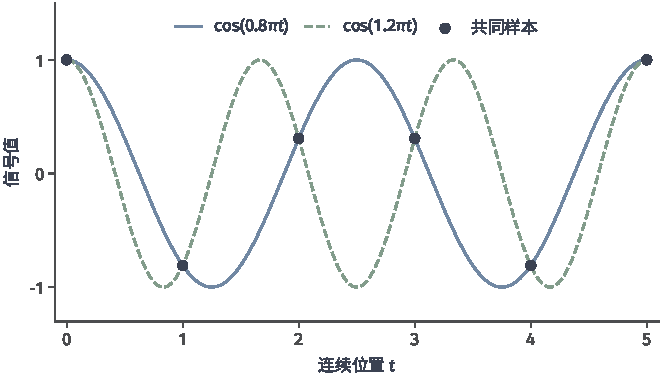
\includegraphics[width=112.0mm]{figures/01-mathematical-preliminaries-upper/07-signals/matplotlib/signal-aliasing-curves/figure.pdf}
  \caption{教学构造$f_1(t)=\cos(0.8\pi t)$与$f_2(t)=\cos(1.2\pi t)$。
  蓝色实线和绿色虚线在整数时刻具有共同样本，深灰圆点标出这些观测。
  图只展示$[0,5]$，样本相同对所有整数成立；两条纯余弦是功率信号，
  不属于后文定理中的整轴平方可积信号类。}
  \label{fig:signal-aliasing-curves}
\end{figure}

任何确定性插值器对相同输入样本都只能返回同一输出，因此不可能同时正确恢复这两条曲线。
学习模型可以凭训练分布猜测更常见的细节，但这种能力来自额外先验，
并不是采样映射自己变成了可逆。这里的余弦只有有限平均功率、整轴能量无穷，
只用于展示歧义；后文将换到$L^2$带限空间，不能把此例当作那个空间中的反例。
对一般$L^2$等价类，点值采样本身还未定义，下一小节会先补齐代表元条件。

离散信号也可以丢弃位置。对正整数$M$保留每$M$项中的一项，
$y[n]=x[Mn]$，称为$M$倍\term{下采样}（downsampling）。其DTFT满足
\begin{equation}
  Y(e^{\mathrm i\omega})=\frac1M\sum_{\ell=0}^{M-1}
  X\left(e^{\mathrm i(\omega+2\pi\ell)/M}\right).
  \label{eq:signal-analysis-downsampling-spectrum}
\end{equation}
对$x\in\ell_1$，按定义展开右侧并交换有限和与绝对收敛级数，
\begin{align*}
  \frac1M\sum_{\ell=0}^{M-1}X\left(e^{\mathrm i(\omega+2\pi\ell)/M}\right)
  &=\sum_{r\in\mathbb Z}x[r]e^{-\mathrm ir\omega/M}
    \left(\frac1M\sum_{\ell=0}^{M-1}e^{-2\pi\mathrm i\ell r/M}\right)\\
  &=\sum_{n\in\mathbb Z}x[Mn]e^{-\mathrm i\omega n}.
\end{align*}
括号内的单位根和只在$M\mid r$时为$1$、否则为$0$，故留下的恰为输出DTFT。
对$x\in\ell_2$，下采样满足$\sum_n|x[Mn]|^2\leq\sum_r|x[r]|^2$，
频域右侧的有限分支映射在$L^2$中也有界；
先对有限截断证明、再取$L^2$极限，便得到同一公式的等价类解释。

输入模式$e^{\mathrm i\omega_0n}$变为$e^{\mathrm iM\omega_0n}$，
输入频率映到$M\omega_0\bmod2\pi$。
原频谱沿输出频率轴扩展$M$倍，超出主值区间的部分回绕，与其他分量相加。
所以“样本点变少”不只是频率曲线画得稀疏，而可能直接合并原来不同的频率。
连续采样的频谱复制也有类似现象，但必须在可读取点值的信号类上推导。

\subsection{带限条件下的信号恢复}
\label{sec:signal-bandlimited-recovery}

前面的歧义来自两条不同频率的曲线具有相同样本。这里通过限制候选曲线允许包含的频率
来排除歧义。直观理由是：样本之所以分不清快波和慢波，是因为采样点太稀，
快波在相邻样本之间多振荡的那一下恰好被错过。只要规定候选信号不含变化过快的分量、
采样点又密到每个慢波“一个完整起伏”都有足够的点记录，这种歧义就能消除。
具体采用带限条件：在某个频率区间之外，频谱几乎处处为零。
\begin{definition}[平方可积带限信号]
  \label{def:signal-analysis-bandlimited-space}
  设$\Omega_{\max}>0$、$f\in L^2(\mathbb R)$，其Plancherel意义的傅里叶变换为$F$。
  若对几乎处处的$|\Omega|>\Omega_{\max}$都有$F(\Omega)=0$，
  称$f$带限于$\Omega_{\max}$。所有这类函数组成
  \term{Paley--Wiener带限空间}。
\end{definition}
只观察一个有限时间窗口，推不出窗口外为零，更推不出高频为零。
带限才是下面用来排除混叠的信号类条件，它必须来自对信号来源的额外了解或测量前的滤波，
而不能从一串有限样本里“看出来”。

这里还顺带解决了一个前面埋下的技术问题：$L^2$函数是按“几乎处处相等”来识别的，
单个点上的值原则上可以任意改动，那“在$t=nT_s$采样”到底取哪个值？
带限条件恰好给出一个确定答案——带限函数自动具有一条连续的版本，采样就针对它进行。
具体地，由$F\in L^2$及频谱支撑长度有限，Cauchy--Schwarz不等式给出
\[
  \|F\|_1\leq\sqrt{2\Omega_{\max}}\,\|F\|_2<\infty.
\]
因此
\[
  f_{\mathrm c}(t)=\frac1{2\pi}\int_{-\Omega_{\max}}^{\Omega_{\max}}
  F(\Omega)e^{\mathrm i\Omega t}\,\mathrm d\Omega
\]
是$f$的连续代表元。若$t_j\to t$，被积函数逐点趋于$F(\Omega)e^{\mathrm i\Omega t}$，
且绝对值都由可积函数$|F|$支配；支配收敛定理使积分值趋于$f_{\mathrm c}(t)$，从而得到连续性。
两个连续代表元若几乎处处相等，就处处相等，所以这种选择唯一。
以下仍把它记为$f$，样本$f(nT_s)$都针对这个代表元，而不针对随意改过点值的版本。

记采样角频率$\Omega_s=2\pi/T_s$，基带$I_s=[-\pi/T_s,\pi/T_s]$。
这里\term{基带}（baseband）指采样后唯一能分辨的那段基本频率区间（频率轴上的一个周期）。
混叠在频域里表现为“频谱被周期性地复制多份、再叠加在一起”：把原频谱每隔$\Omega_s$
抄一份，按
\[
  P_F(\Omega)=\frac1{T_s}\sum_{k\in\mathbb Z}F(\Omega-k\Omega_s).
\]
相加。采样越密（$T_s$越小、$\Omega_s$越大），这些副本隔得越开；
采样够密时副本互不重叠，基带里就只剩原频谱本身，这正是不混叠的频域表现。
由于$F$带限，在$I_s$上只有有限多个平移副本可能非零，故$P_F\in L^2(I_s)$，并以$\Omega_s$为周期。
采用基$e^{-\mathrm i\Omega nT_s}$，其第$n$个傅里叶系数为
\begin{align*}
  \frac1{\Omega_s}\int_{I_s}P_F(\Omega)e^{\mathrm i\Omega nT_s}\,\mathrm d\Omega
  &=\frac1{2\pi}\int_{\mathbb R}F(\Omega)e^{\mathrm i\Omega nT_s}\,\mathrm d\Omega\\
  &=f(nT_s)=x[n].
\end{align*}
第一步令$u=\Omega-k\Omega_s$，各平移区间拼回实轴，
且$e^{\mathrm inT_sk\Omega_s}=e^{2\pi\mathrm ink}=1$；
第二步就是所选连续代表元的逆变换。
由周期Parseval关系，系数序列$x$属于$\ell_2$，故样本的频率表示
$X_s(\Omega)=\sum_n x[n]e^{-\mathrm i\Omega nT_s}$在$L^2(I_s)$中有定义。
它与$P_F$的全部系数相同，得到
\begin{equation}
  X_s(\Omega)=\frac1{T_s}\sum_{k\in\mathbb Z}F(\Omega-k\Omega_s).
  \label{eq:signal-analysis-spectral-replication}
\end{equation}
这也就是DTFT在$\omega=\Omega T_s$下的写法。
采样不是只保留一份原频谱，而是周期复制再叠加。
以上推导只用带限空间、傅里叶级数和积分，不需要把采样写成Dirac脉冲列的乘积；
若采用后者，则要另行建立广义函数的乘积与变换规则。

现在可以从频域看清混叠发生与否的分界。当$\Omega_s>2\Omega_{\max}$时，相邻副本之间留有空隙、
互不重叠，基带内只有中央那一份原频谱，采样保留了全部信息。
当$\Omega_s<2\Omega_{\max}$时，允许频带与它的平移副本会在一段非零长度的区间上重叠相加；
更糟的是可以构造出一个非零信号，它的两份频谱副本在每个频率处正好正负抵消，
于是全部样本竟然都是零——这说明此时存在“非零信号却采成全零”，采样不可逆。
构造方法是在频带内选一个小区间$J$，使$J$和$J+\Omega_s$都落在频带中且互不相交；
在$J$上放任意非零$L^2$频谱、在$J+\Omega_s$上放它的负平移，周期复制后即相消。
临界情形$\Omega_s=2\Omega_{\max}$两份副本只在端点相碰，
零测端点不改变当前$L^2$等价类，不能把它与正测度重叠一概而论。

图~\ref{fig:vol1-add-signal-spectral-replicas}把同一条三角形频谱按两种采样角频率复制。
采样较疏时副本间隔缩小，基带中的频谱值便可能同时包含来自不同原频率的贡献；
这正是频谱复制式中的相加，而不是原频谱只少画了几个点。
\begin{figure}[!htb]
  \centering
  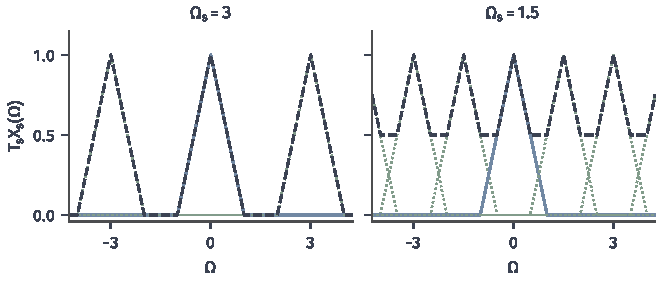
\includegraphics[width=112mm]{figures/01-mathematical-preliminaries-upper/07-signals/matplotlib/comprehension-additions/signal-spectral-replicas.pdf}
  \caption{教学频谱$F(\Omega)=\max\{1-|\Omega|,0\}$的周期复制，带宽为$\Omega_{\max}=1$。
  蓝实线是中央副本，绿点线是平移副本，深灰虚线为其总和$T_sX_s(\Omega)$；横轴为角频率。
  左侧$\Omega_s=3>2$时副本分离，右侧$\Omega_s=1.5<2$时相邻副本在非零长度区间重叠。
  纵轴乘以$T_s$以保留原频谱的幅值尺度，实际$X_s$还包含$1/T_s$因子。}
  \label{fig:vol1-add-signal-spectral-replicas}
\end{figure}

\begin{theorem}[带限信号的采样重构]
  \label{thm:signal-analysis-sampling}
  若$f$属于上述Paley--Wiener空间，频谱支撑包含于$[-\Omega_{\max},\Omega_{\max}]$，
  且$\Omega_s>2\Omega_{\max}$，则全部样本$f(nT_s)$唯一确定$f$，并有
  \begin{equation}
    f(t)=\sum_{n\in\mathbb Z}f(nT_s)
    \operatorname{sinc}\left(\frac{t-nT_s}{T_s}\right),
    \qquad \operatorname{sinc}(u)=\frac{\sin(\pi u)}{\pi u},
    \label{eq:signal-analysis-sinc-reconstruction}
  \end{equation}
  其中$\operatorname{sinc}(0)=1$。对称部分和在$L^2(\mathbb R)$中收敛，
  并对所选连续代表元在整条实轴上一致收敛。
\end{theorem}
\begin{proof}
  条件保证$F$的支撑严格落在$I_s$内，频谱复制式在该区间上给出$F=T_sX_s$。
  因此$F$相对于$e^{-\mathrm i\Omega nT_s}$的傅里叶系数是$T_sf(nT_s)$，部分和
  \[
    F_K(\Omega)=T_s\sum_{n=-K}^{K}f(nT_s)e^{-\mathrm i\Omega nT_s}
  \]
  在$L^2(I_s)$中趋于$F$。这里把原本只占较窄频带$[-\Omega_{\max},\Omega_{\max}]$的$F$
  视为更大空间$L^2(I_s)$中的元素，在多出的频率位置上其值为零。展开所用的基可以覆盖整个$I_s$；
  单个重构项或有限部分和不必仍局限于原来的较窄频带，全部系数在$L^2$极限中才恢复带外的零值。
  把$F_K$在$I_s$外取零，逆变换的有限和可移到积分外：
  \begin{align*}
    f_K(t)
    &=\sum_{n=-K}^{K}f(nT_s)\frac{T_s}{2\pi}
      \int_{-\pi/T_s}^{\pi/T_s}e^{\mathrm i\Omega(t-nT_s)}\,\mathrm d\Omega\\
    &=\sum_{n=-K}^{K}f(nT_s)
      \operatorname{sinc}\left(\frac{t-nT_s}{T_s}\right).
  \end{align*}
  对$t\neq nT_s$，指数积分是$2\sin(\pi(t-nT_s)/T_s)/(t-nT_s)$；
  当$t=nT_s$时积分为区间长度$2\pi/T_s$，乘上$T_s/(2\pi)$后才等于$1$，
  与$\operatorname{sinc}(0)=1$的连续延拓一致。
  Plancherel等式给出
  $\|f_K-f\|_2=(2\pi)^{-1/2}\|F_K-F\|_2\to0$，从而得到$L^2$重构。

  虽然有限部分和未必保持原来的窄频带，但$F_K-F$始终支持在同一个有限区间$I_s$内。
  因此一个与$t$无关的点值界就能控制全部时刻的误差：
  \[
    \sup_{t\in\mathbb R}|f_K(t)-f(t)|
    \leq\frac1{2\pi}\|F_K-F\|_{L^1(I_s)}
    \leq\frac{\sqrt{|I_s|}}{2\pi}\|F_K-F\|_{L^2(I_s)}
    \longrightarrow0.
  \]
  这证明整轴一致收敛。所用关键是有限频谱支撑，
  不能把这项结论直接套到任意周期$L^2$函数的逐点傅里叶展开。

  若两条满足条件的信号样本相同，则频谱在$I_s$上的所有傅里叶系数相同。
  完备性使两频谱几乎处处相等，逆变换后得到同一$L^2$元素及同一连续代表元，因而恢复唯一。
\end{proof}

重建公式为什么恰好取sinc这种形状，可以从“每个样本各管一段、互不干扰”来理解。
sinc在自己的中心（原点）取值为$1$，在其他所有整数采样点恰好为零。于是把每个样本值乘上
以该样本为中心的sinc波形后，这条波形只在自己的中心贡献该样本值、在其他样本点贡献$0$；
把所有这些波形叠加，曲线自然穿过每一个给定样本，而样本之间取什么值则由带限性唯一确定。
所以“插值穿过所有样本”这一点看图就能验证，但“样本之间恰好等于原函数、不存在另一条
也穿过这些点的带限曲线”靠的是带限性与刚才的唯一性证明，不能只凭插值成立就下结论。
由基带Parseval还可得$\|f\|_2^2=T_s\sum_n|f(nT_s)|^2$，
说明在当前条件下，连续能量与离散样本能量只差一个采样间隔因子。

定理用严格不等号留下频率余量。同一证明可在当前$L^2$模型中按几乎处处意义延伸到
$\Omega_s=2\Omega_{\max}$，端点相接无碍。
若扩大到允许谱线的功率信号，临界点要另行处理：
$\sin(\Omega_{\max}t)$在$T_s=\pi/\Omega_{\max}$的全部样本为零，
但它不属于$L^2(\mathbb R)$，因此并不反驳此处结论。

图~\ref{fig:vol1-add-signal-sinc-cardinal}给出当前$L^2$模型中的一个临界带限构造，
直接显示每个样本怎样控制一个sinc项：在其他整数位置该项均为零，
三个项的和便能分别保留三个非零样本，而不改动其余整数位置的零值。
\begin{figure}[!htb]
  \centering
  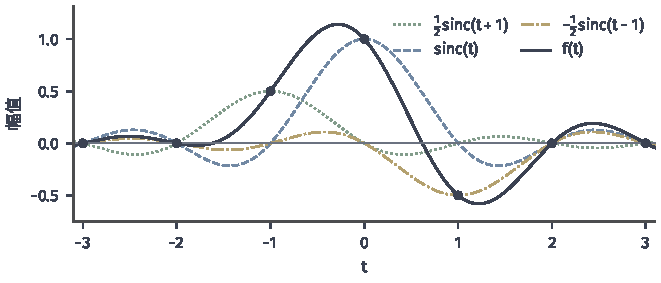
\includegraphics[width=112mm]{figures/01-mathematical-preliminaries-upper/07-signals/matplotlib/comprehension-additions/signal-sinc-cardinal.pdf}
  \caption{取$T_s=1$并构造$f(t)=\tfrac12\operatorname{sinc}(t+1)+\operatorname{sinc}(t)
  -\tfrac12\operatorname{sinc}(t-1)$。
  三条彩色曲线是三个样本对应的加权sinc项，深灰实线为其和，圆点标出整数样本。
  该函数平方可积、带限于$\pi$，全部整数样本只有$-1,0,1$处分别为$\tfrac12,1,-\tfrac12$，其余均为零。
  这是按有限个sinc项精确定义的信号，不是把任意无限样本记录截断后仍宣称精确恢复。}
  \label{fig:vol1-add-signal-sinc-cardinal}
\end{figure}

定理使用全部双向无限样本，理想sinc也有无限支撑。
有限时长、噪声、未知带宽及非带限分量不会因公式而消失；
有限记录只能支持截断或其他有条件的近似重构，不能宣称享有同样的无误差保证。
把有限窗口外补零还会改变原信号，不能用这个人为边界代替带限假设。

\subsection{降采样前的抗混叠处理}

若原信号含有将在抽取后重叠的频率，就应在下采样前先限制这些分量，
这种预处理称为\term{抗混叠滤波}（anti-aliasing filtering）。
它的必要性可直接从上一小节推出：一旦高频分量在抽取后折回并与低频重叠，
任何事后处理都无法再把二者分开，因为数组里看到的本就是同一组样本；
所以必须在“信息尚未被合并”之前，先把会造成混淆的高频压低。
对$M$倍下采样，理想低通把频率支持限制到$|\omega|<\pi/M$内，
使式~\eqref{eq:signal-analysis-downsampling-spectrum}中的频谱副本不混在一起。
这里恢复的目标是预滤波后的信号，而不是已被滤掉的全部原信号。
设计时把希望保留的频段称为通带（passband）、希望压低的频段称为阻带（stopband）；
这些名称描述对频率响应的要求，并不表示实际滤波器已经满足要求。

局部平均提供了容易计算的平滑，却不自动满足理想低通条件。长度$M\geq1$的均值核为
$h[n]=1/M$（$0\leq n<M$），其余为零。由有限几何级数，
\[
  H(e^{\mathrm i\omega})=\frac1M\sum_{n=0}^{M-1}e^{-\mathrm i\omega n}
  =\frac1M\frac{1-e^{-\mathrm iM\omega}}{1-e^{-\mathrm i\omega}},
\]
再从分子分母各提出中间相位因子，得到
\begin{equation}
  H(e^{\mathrm i\omega})=
  \frac1M e^{-\mathrm i\omega(M-1)/2}
  \frac{\sin(M\omega/2)}{\sin(\omega/2)}.
  \label{eq:signal-analysis-moving-average-response}
\end{equation}
当$\omega\in2\pi\mathbb Z$出现$0/0$时，按原有限和取连续值$1$。
当$M\geq2$时，该响应有衰减和零点，却不能把一整段阻带频率都消去。
当$M\geq3$时，在主频率区间$[-\pi,\pi]$内还能看到主峰以外的小峰，
称为旁瓣（sidelobes），它们直接显示了高频残留。
图~\ref{fig:vol1-add-signal-mean-response}把长度不同的均值核分别与同倍率下采样
所需的频带限制比较。即使响应出现零点，两个零点之间仍可有非零响应，
因此不能用“存在零点”替代“整个待抑制频段为零”。
\begin{figure}[!htb]
  \centering
  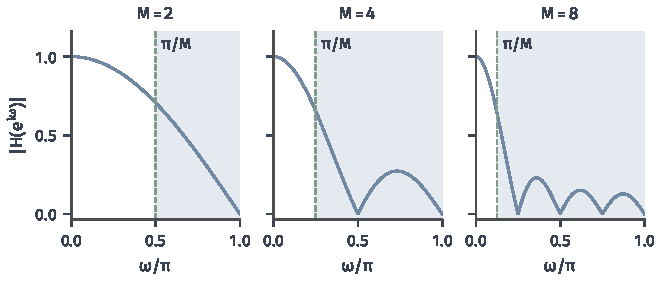
\includegraphics[width=112mm]{figures/01-mathematical-preliminaries-upper/07-signals/matplotlib/comprehension-additions/signal-mean-response.pdf}
  \caption{长度$M=2,4,8$的因果均值核在$0\leq\omega\leq\pi$上的幅频响应。
  绿虚线标出$\omega=\pi/M$，浅蓝区是$M$倍下采样前理想频带限制之外的正频率部分。
  均值核的幅值在这一区域内仍可能非零；增加窗口长度会改变零点与旁瓣，却不会把整个区域全部消去。
  各面板共用幅值和归一化频率尺度，未展示的负频率部分与正频率部分关于$\omega=0$轴对称。}
  \label{fig:vol1-add-signal-mean-response}
\end{figure}

相位因子反映以当前及过去样本实现均值时的时间对齐；按窗口输出的平均池化
（average pooling）可看成这种滤波后抽取。具体地，对实序列和同一长度$M$窗口，
平均池化和最大池化（max pooling）分别为
\[
 \begin{aligned}
  p_{\mathrm{avg}}[m]&=\frac1M\sum_{r=0}^{M-1}x[Mm+r],\\
  p_{\mathrm{max}}[m]&=\max_{0\leq r<M}x[Mm+r].
 \end{aligned}
\]
若$y=x*h$使用前述因果均值核，则$p_{\mathrm{avg}}[m]=y[Mm+M-1]$，
窗口起点与卷积输出时刻之间有明确的索引偏移。
当$M\geq2$时，最大池化不满足线性叠加：先取长度二的窗口，$(1,0)$和$(0,1)$的最大值都是$1$，
相加后的窗口$(1,1)$最大值仍是$1$，并非两个输出之和$2$；把更长窗口在其余位置补零，仍给出同一反例。
因此长度至少为二的最大池化不能用一个固定线性频率响应完整描述；长度一时它只是恒等映射。

为直接看到高频残留，固定同一个两频输入，比较直接抽取、理想低通和均值预滤波：
\[
  x[n]=\cos(0.2\pi n)+\sin(0.8\pi n).
\]
直接二倍抽取得到$x[2m]=\cos(0.4\pi m)-\sin(0.4\pi m)$，
因为$1.6\pi m=2\pi m-0.4\pi m$，原高频正弦折回到低频。
若先理想低通、完全删除$0.8\pi$分量，输出为$\cos(0.4\pi m)$。
若仅用$h=(1/2,1/2)$，令$y[n]=(x[n]+x[n-1])/2$，本例取偶数位置$q[m]=y[2m]$。
它与前文长度二平均池化所取的$y[2m+1]$相差一个抽取位置。两项分别用和差化积公式，得到
\[
 \begin{aligned}
  q[m]={}&\cos(0.1\pi)\cos(0.4\pi m-0.1\pi)\\
        &+\cos(0.4\pi)\sin(1.6\pi m-0.4\pi).
 \end{aligned}
\]
第一项是原低频经过均值滤波后的结果，幅度和相位都已改变；
第二项来自原高频，抽取后仍折回低频。均值滤波在原高频处的残留幅度为
\[
  |H(e^{\mathrm i0.8\pi})|=\cos(0.4\pi)>0,
\]
所以局部平均只削弱了这个分量，并没有清除它。

在$m=0$处可分别复算两项贡献：低频为
$(1+\cos(0.2\pi))/2\approx0.904508$，高频为
$-\sin(0.8\pi)/2\approx-0.293893$，相加得$q[0]\approx0.610616$，
而理想低通输出为$1$。非零的第二项直接显示了混叠残留；
总输出与$1$的差则同时包含通带的幅度/相位误差和高频残留，不能全部归因于混叠。

某一组输出重合也不能代替这个频率响应检查。例如换成
\[
 \begin{aligned}
  \widetilde x[n]&=\cos(0.2\pi n)+\cos(0.8\pi n)\\
                 &=(1+(-1)^n)\cos(0.2\pi n).
 \end{aligned}
\]
此时奇数位置全为零。同样的“均值后偶数抽取”就恰好给出$\cos(0.4\pi m)$，
与理想低通输出相同。这个抵消依赖特定输入的相位和幅值；判断滤波器是否满足抗混叠条件，
仍需检查整个允许输入类，而不能只看一次相同输出。
这些纯正弦、余弦用于按模式计算频率响应，是功率信号算例，不属于前述$L^2$恢复定理的信号类。
“已经平滑”与“满足无混叠的带限条件”因而是两种不同的保证。

那为什么不能干脆设计一个“通带内增益全为$1$、阻带内增益全为$0$”的理想低通，
把高频一次性清零？原因在于这样的核必须无限长。有限长度核的频率响应是有限个复指数的线性组合，
也称三角多项式。令$z=e^{-\mathrm i\omega}$，该响应可写成有限个整数幂$z^r$之和；
若有负幂，乘以适当的$z$次幂即可化为普通多项式，而单位圆上$z\neq0$。
一整段非零长度的频率区间给出无限多个不同的$z$，若响应在这里为零，
对应多项式就有无限多个根；但非零有限次数多项式的根数有限，故该多项式只能恒为零，
与“通带为$1$”矛盾。
这一段结论对实践很重要：用有限长的核做预滤波，注定只能把混叠压小、不能彻底清零，
所以要在“保留多少低频细节”和“残留多少高频混叠”之间权衡。实际设计通常允许
通带与阻带之间留一段缓变的过渡带（transition band）。通带误差衡量保留频段偏离目标多少，
阻带衰减衡量抑制频段还剩多大幅度；它们要与过渡带宽度、延迟及计算量一起规定。
滤波后剩余的混叠是设计误差的一部分，不能因用了“低通”名称就忽略。
如果响应在某频段为零，该频段进入映射的零空间：这部分输入差别在输出里彻底看不见；
接近零的响应虽可能形式可逆，但反演时要把微小输出放大，噪声也随之被放大。
第~\ref{chap:linear-algebra-and-matrix-analysis}章
“线性空间”中的零空间与小奇异值分析在这里仍然适用：
前者说明哪些输入区别完全不可见，后者说明哪些区别虽可见却难以稳定恢复。

除了截止位置，核的形状也决定它怎样改变空间读数。归一化高斯核的连续频率响应为
$e^{-\sigma^2\|\bm\Omega\|^2/2}$。在一维，高斯积分由二维极坐标给出归一化常数；
对频率求导并对空间分部积分，有$F'(\Omega)=-\sigma^2\Omega F(\Omega)$、$F(0)=1$，
解此一阶方程得到该响应，多维再逐轴相乘。因此空间越宽，频率响应越窄；
这是同一个参数在两个坐标中的反向尺度关系。高斯核非负且积分为$1$，
对有界实输入的输出是其值的加权平均，必在输入的上下界之间。

硬截止的频率权重即使都为零或一，其空间核也可能变号。有限循环例子能直接显示后果：
$N=4$时保留频率$0,1,3$、去掉频率$2$，逆DFT核为$h=(3/4,1/4,-1/4,1/4)$。
输入$(1,0,0,0)$产生负读数$-1/4$；输入$(0,1,1,1)$则在相应位置产生$5/4$。
超出原值范围的振荡来自变号权重，不能只看“低通”名称就断言不会超调。
平缓截止、非负平均、频率选择性和有限核长度是不同约束，
设计滤波器时要说明当前要控制哪一种误差。

\subsection{多维与时空网格上的采样}
\label{sec:signal-multidimensional-sampling}

一维采样按时间区分频率，图像与视频还要同时区分多个空间方向和时间。
新增的困难是：不同方向的高频可以在同一采样格上变成低频，
面积或曝光平均又会在采样之前削弱某些频率。
我们先确定哪些频率在网格上无法区分，再把已有恢复结论逐轴使用，
最后把像素面积与运动放回同一相位计算。

\subsubsection{采样格与逐轴带限}
规则采样点为$\bm t=\bm A\bm n$，其中$\bm A$可逆、$\bm n\in\mathbb Z^d$。
复指数$e^{\mathrm i\bm\Omega^\top\bm t}$与频率
$\bm\Omega+2\pi\bm A^{-\top}\bm k$在这些点的值完全相同，因为新增相位为$2\pi\bm k^\top\bm n$。
这个关系描述一般\term{采样格}（sampling lattice）的频率歧义。
对$\bm A=\operatorname{diag}(T_1,\ldots,T_d)$，
每个频率分量分别按$2\pi/T_j$混同，中央矩形区域为$|\Omega_j|<\pi/T_j$。
二维以每像素周期数记频率时，$\cos(2\pi(un_1+vn_2))$与$(u+k,v+\ell)$产生相同样本。
例如$(u,v)=(0.6,0.1)$与$(-0.4,0.1)$无法区分，变化的表观方向也可能不同；
这就是规则纹理出现摩尔纹的一个确定性来源。

对傅里叶支撑位于该矩形内的$L^2(\mathbb R^d)$函数，
支撑有限保证其频谱也在$L^1$，从而选定连续代表元$f_{\mathrm c}$。
把一维傅里叶级数与sinc正交展开在每个坐标各用一次，得到
\begin{equation}
 f_{\mathrm c}(\bm t)=
 \sum_{\bm n\in\mathbb Z^d}
 f_{\mathrm c}(T_1n_1,\ldots,T_dn_d)
 \prod_{j=1}^d\operatorname{sinc}(t_j/T_j-n_j).
 \label{eq:signal-multidimensional-sinc}
\end{equation}
矩形部分和先在$L^2$中收敛；带限空间上点值由频谱的$L^2$范数控制，
所以也恢复所选连续代表元的各点。这只是已有一维证明的张量积：
频谱矩形上的正交基是各轴基函数的乘积，其系数就是带尺度因子的网格样本。
它要求整格无限样本与指定带限类，不把有限图像自动变成无限分辨率对象。
矩形限制是方便的充分条件；其他频谱支撑须检查其按对偶采样格平移后是否重叠，
不能只用一个“最高频率的模长”代替全部方向。

每轴抽取$M_j$倍时，也可对原一维DTFT混叠式逐轴换元，得到$\prod_jM_j$个频谱副本的平均。
因此各轴截止应匹配各自抽取率；把宽、高压缩到不同倍数时，
只按一个轴设计低通会遗漏另一个轴的混叠。

\subsubsection{面积平均与运动相位}
真实相机的一个像素并不是空间中的一个点，而是覆盖一小块感光面积，把这块面积内的光平均后
才记成一个读数；视频的一帧也经历了一小段曝光时间。因此在“采样取点”之前，
信号已经先被这些有限尺寸平均过一次。像素若记录中心附近宽$a_j$的长方体平均，
采样前就先与一个归一化盒形核卷积。把复指数放入这一平均，每轴直接积分给出
\begin{equation}
 B(\bm\Omega)=
 \prod_{j=1}^d\frac{\sin(\Omega_ja_j/2)}{\Omega_ja_j/2}.
 \label{eq:signal-box-aperture-response}
\end{equation}
零分量处取极限$1$。每个方向的零点与旁瓣说明面积平均并非理想砖墙低通，
在采样界之外仍可能留下贡献；它也已经改变了待恢复的对象。
这与前述有限移动平均的频率响应是连续、离散两种版本。
时长$\tau$的对称曝光平均，在时间角频率$\omega$处再乘
$\sin(\omega\tau/2)/(\omega\tau/2)$，并不是在每个频率上都同样衰减。

视频里还有一个更直观的混叠——车轮在镜头中可能看起来倒转。根源是空间条纹与拍摄帧率
共同决定了时间频率。对以速度$\bm v$移动的空间平面波
$f(\bm x,t)=\cos(2\pi\bm u^\top(\bm x-\bm v t))$，在固定位置观察，
它随时间的振荡频率为$-\bm u^\top\bm v$（条纹扫过该点的速度）。
空间采样与帧率$f_s$分别限制$\bm u$的各分量和$|\bm u^\top\bm v|<f_s/2$。
例如条纹频率$0.4$周期/像素、沿法向速度$2$像素/帧时，
每帧变化$0.8$周，与$-0.2$周有同一样本，表观运动可能反向。
这些余弦是用来展示歧义的功率信号，不属于前述整轴$L^2$恢复定理的对象。
运动、空间尺度、曝光及采样的条件须共同给定。

\subsection{插零后的频谱与插值}
\label{sec:signal-upsampling-interpolation}

想提高图像分辨率时，最容易产生的误解是：在原有像素之间插入更多位置，
是不是就“补出”了原来没拍到的细节？并不是。新位置上没有真实读数，
在给出一条填补规则之前，它们不携带任何信息。为把这一步说清楚，要区分两个动作：
先在新位置放零（插零），再用一个插值核根据周围旧读数算出新位置的值。
先用整轴离散变换看清插零会产生哪些频谱副本，再检查插值核能消去哪些副本、
以及它是否保留原有读数和常量背景。

对正整数$L$，令$u[Ln]=x[n]$，其余位置为零。对$x\in\ell_1$直接改变求和索引，得到
\begin{equation}
 U(e^{\mathrm i\omega})=X(e^{\mathrm iL\omega}),\qquad
 Y(e^{\mathrm i\omega})=H(e^{\mathrm i\omega})X(e^{\mathrm iL\omega}),
 \label{eq:signal-upsampling-spectrum}
\end{equation}
第二式是$y=h*u$的频域表达。原谱按频率压缩$L$倍，并在一个$2\pi$周期内出现$L$份。
若希望选择中央一份，理想插值响应在$|\omega|<\pi/L$取$L$、其余取零；
该响应的增益补偿插零后密度的降低。其核为$\operatorname{sinc}(n/L)$，
通常不绝对可和，所以理想情形须按带限$L^2$展开或有限能量离散变换理解，
不能直接套用上面$\ell_1$核的充分条件。实际有限插值核只近似这个选频过程，
会留下相应的过渡与镜像误差。

保留旧格点的插值条件是$h[Ln]=\mathbb I_{\{0\}}[n]$。
保常量的条件则是对每个相位$r=0,\ldots,L-1$，$\sum_qh[r-Lq]=1$。
二者回答不同问题。例如$L=2$的核$h[-1]=h[1]=1/2$、$h[0]=1$，
在旧格点复制原值、在两点之间取平均，同时保常量。
把$x=(2,4)$放到零延拓的整轴上，在内部新位置得到$3$；
边缘新位置是否仍为端值，还取决于零延拓或复制延拓。
二维插零与插值逐轴进行，频谱复制数和增益分别相乘；
这些新读数由假设的核决定，不能当成新增的独立观测。

\section{本章小结}
\label{sec:signal-analysis-summary}

分析信号先要确定在哪里取值、每个位置有几个通道，以及首尾如何连接。
有限记录不等于有限支撑，通道数不等于时间长度，周期延拓也不等于原过程周期。
内积规定比较口径，范数与能量衡量累计大小，平均功率则适合长期持续的信号；
改变通道权重或观察窗口，比较的对象也随之改变。

脉冲、傅里叶和多项式表示从不同方向描述同一信号。
完整有限DFT及满足次数条件的插值可以无损恢复坐标；无穷傅里叶展开则需要说明
积分、均方或逐点意义。幅度不包含全部位置信息，Parseval中的尺度因子来自归一化，
截断系数才引入相应的表示误差。多维变换逐轴继承这些坐标关系；
反射余弦表示改变边界，短时频谱增加局部位置，却也引入窗口泄漏和分辨能力的限制。
只保存幅度、频带和或部分系数时，原来的全坐标可逆性不再自动保留。

平移、反转、幅值缩放与时间缩放改变的是不同属性。
线性与平移不变使有限支撑输入的输出可写成与脉冲响应的卷积，
无穷输入还需有界性或可积条件。时变核可以线性却不只依赖滞后，输入门控通常破坏叠加；
多通道矩阵核还要分清时间汇总与通道混合。相关按原模板方向比较局部片段，
不能只凭实现名称把它与卷积混同。矩阵化集中局部点积，
FFT、Toom--Cook和Winograd用不同表示减少同一目标的计算，空间可分离核则依赖低秩结构；
核方向、边界、输出范围及数值条件仍由目标决定。
网格差分以步长和光滑性联系导数，Haar分解用正交细节保留变化，
滤波器组靠混叠消去重建，金字塔则靠保存残差逐层重建。
量化改变可存储的幅度，闭环差值编码需要两端共享重建历史；
集合开闭依据包含与伴随关系，其局部极值实现不能当成线性卷积。

采样最后改变的是可用信息。不同信号可能具有同一样本，坐标可逆和计算快速
都补不回已经消失的区别。带限有限能量类、规范连续代表元及足够密的无限样本共同给出sinc恢复；
有限记录和功率信号需要各自核对边界。抗混叠预滤波可以控制即将重叠的频率，却也改变待恢复的目标。
多维网格要逐方向检查混叠，视频还需把运动引起的时间相位与空间频率一起检查。
插零后滤波只按已有样本和插值规则生成新读数，不能增加独立观测。
随机模型描述观测中的不确定性，内部状态演化则可以进一步构造响应核；
本章的输入输出视角会继续用于判断这些响应怎样作用于信号。
下一章把规则索引推广为一般图：连接关系决定哪些位置可以比较与传播，
图上的谱则提供相应的变化坐标。

